\setcounter{section}{0}% Change the value of the chapter counter
%\numberwithin{equation}{chapter}% Equation counter subordinated to the section counter
\numberwithin{equation}{section}% Equation counter subordinated to the section counter
\numberwithin{figure}{section}% Figure counter subordinated to the section counter
\setcounter{chapter}{9}
\chapter{\texorpdfstring{Type I and Type II Superstrings}{10 Type I and Type II Superstrings}} \label{cha:10}


\section{Superconformal Algebra}

In the bosonic string, the mass-shell condition
\begin{equation}
	p_{\mu}p^{\mu}+m^{2}=0 \label{10.1.1}
\end{equation}
comes from the physical state condition
\begin{equation}
	L_{0}\lvert \psi\rangle = 0\: , \label{10.1.2}
\end{equation}
and in the closed string, $\tilde{L}_{0}\lvert\psi\rangle=0$ must also be added. To obtain fermions, we need the Dirac equation
\begin{equation}
	\mi p_{\mu} \Gamma^{\mu}+m=0\:. \label{10.1.3}
\end{equation}

In the bosonic string, $L_{0}$ and $\tilde{L}_{0}$ are the center-of-mass modes of the energy-momentum tensor $(T_{B},\tilde{T}_{B})$. Now we want to introduce new conserved quantities $T_{F}$ and $\tilde{T}_{F}$, such that their center-of-mass modes yield the Dirac equation. Note that since the spacetime momentum $p^{\mu}$ is the center-of-mass mode of the worldsheet currents $(\partial X^{\mu},\bar{\partial}X^{\mu})$, we now expect the $\Gamma$ matrices satisfying the algebra
\begin{equation}
	\{\Gamma^{\mu},\Gamma^{\nu}\}=2\eta^{\mu\nu} \:, \label{10.1.4}
\end{equation}
to be the center-of-mass modes of the anticommuting worldsheet fields $\psi^{\mu}$.

Now let us examine the worldsheet action
\begin{equation}
	S=\frac{1}{4\uppi}\int\dif^{2}z \:
	\left(
	\frac{2}{\alpha^{\prime}}\partial X^{\mu}\bar{\partial}X_{\mu} +\psi^{\mu}\bar{\partial}\psi_{\mu}
	+\tilde{\psi}^{\mu}\partial\tilde{\psi}_{\mu}
	\right)\:.\label{10.1.5}
\end{equation}
The OPE of $XX$ is
\begin{equation}
	X^{\mu}(z,\bar{z})X^{\nu}(0,0)\sim -\frac{\alpha^{\prime}}{2}\eta^{\mu\nu}\ln\lvert z\rvert^{2}\:.\label{10.1.6}
\end{equation}
$\psi$ and $\tilde{\psi}$ are holomorphic and antiholomorphic, respectively, and their OPEs are
\begin{equation}
	\psi^{\mu}(z)\psi^{\nu}(0)\sim\frac{\eta^{\mu\nu}}{z}\:,\qquad
	\tilde{\psi}^{\mu}(\bar{z})\tilde{\psi}^{\nu}(0)\sim\frac{\eta^{\mu\nu}}{\bar{z}}\: \label{10.1.7}
\end{equation}
The \emph{worldsheet supercurrents} are
\begin{equation}
	T_{F}(z)=\mi(2/\alpha^{\prime})^{1/2}\psi^{\mu}(z)\partial X_{\mu}(z)\:,\qquad
	\tilde{T}_{F}(\bar{z})=\mi(2/\alpha^{\prime})^{1/2}\tilde{\psi}^{\mu}(\bar{z})\bar{\partial} X_{\mu}(\bar{z})
	\:.\label{10.1.8}
\end{equation}
\begin{tcolorbox}[breakable]
\begin{proof}
		We consider the left-moving part of the action
		\begin{equation}
			S_L=\frac{1}{4\pi}\int d^2z\left(\frac{2}{\alpha'}\partial X^\mu \bar\partial X_\mu+\psi^\mu\bar\partial\psi_\mu\right).
		\end{equation}
		
		We take a local supersymmetry transformation with parameter $\epsilon(z,\bar z)$:
		\begin{align}
			\delta X^\mu &= \epsilon(z,\bar z)\,\psi^\mu, \\
			\delta \psi^\mu &= -\frac{2}{\alpha'}\,\epsilon(z,\bar z)\,\partial X^\mu.
		\end{align}

		Because the grassmann variables anti-commute, we have
		\begin{equation}
			\delta\!\left(\int \psi^\mu \bar\partial \psi_\mu\right)
			= 2 \int \delta\psi^\mu\,\bar\partial \psi_\mu,
		\end{equation}
		up to boundary terms. Hence
		\begin{align}
			\delta S_\psi
			&= \frac{1}{2\pi}\int d^2z\, \delta\psi^\mu\,\bar\partial \psi_\mu= -\frac{1}{2\pi\alpha'}\int d^2z\, 2\mathcolor{red}{\epsilon\,\partial X^\mu\,\bar\partial \psi_\mu}.
		\end{align}
		The bosonic part can be given as:
		\begin{align}
			\delta S_X
			&= \frac{1}{4\pi}\int d^2z\,\frac{2}{\alpha'}
			\left(\partial(\epsilon\psi^\mu)\bar\partial X_\mu + \partial X^\mu \bar\partial(\epsilon\psi_\mu)\right).
		\end{align}
		Using
		\begin{align}
			\partial(\epsilon\psi^\mu) &= (\partial \epsilon)\psi^\mu + \epsilon\,\partial \psi^\mu, \\
			\bar\partial(\epsilon\psi^\mu) &= (\bar\partial \epsilon)\psi^\mu + \epsilon\,\bar\partial \psi^\mu.
		\end{align}
		We have:
		\begin{align}
			\delta S_X
			= \frac{1}{2\pi\alpha'}\int d^2z \Big[
			(\partial\epsilon)\psi^\mu\bar\partial X_\mu
			+ \epsilon\,\partial\psi^\mu\bar\partial X_\mu + (\bar\partial\epsilon)\psi^\mu\partial X_\mu
			+\mathcolor{red}{ \epsilon\,\partial X^\mu\bar\partial\psi_\mu}
			\Big].
		\end{align}
		Adding $\delta S_X$ and $\delta S_\psi$:
		\begin{align}
			\delta S
			= \frac{1}{2\pi\alpha'}\int d^2z \Big[
			(\partial\epsilon)\psi^\mu\bar\partial X_\mu
			+ (\bar\partial\epsilon)\psi^\mu\partial X_\mu  + \epsilon\big(\partial\psi^\mu\bar\partial X_\mu - \partial X^\mu\bar\partial\psi_\mu\big)
			\Big].
		\end{align}
		From Integration by parts, we have:
		
		\begin{align}
			\int (\partial\epsilon)\psi^\mu\bar\partial X_\mu
			&= -\int \epsilon\,\partial(\psi^\mu\bar\partial X_\mu) \\
			&= -\int \epsilon\big(\partial\psi^\mu\bar\partial X_\mu + \psi^\mu \partial\bar\partial X_\mu\big).
		\end{align}
		
		Using $\partial\bar\partial X_\mu = \bar\partial\partial X_\mu$, and dropping the total derivative-terms. We are left with
		\begin{align*}
			\delta S
			&= \frac{1}{2\pi\alpha'}\int d^2z \Big[
			-\cancel{\epsilon\partial\psi^\mu\bar\partial X_\mu} + \bar\partial\epsilon\psi^\mu \partial X_\mu+\cancel{\epsilon\partial X^\mu\bar\partial\psi_\mu}
			+ (\bar\partial\epsilon)\psi^\mu\partial X_\mu \\
			&\qquad + \epsilon\big(\cancel{\partial\psi^\mu\bar\partial X_\mu} - \cancel{\partial X^\mu\bar\partial\psi_\mu}\big)
			\Big]\\
			&= \frac{1}{2\pi}\int d^2z\,(\bar\partial \epsilon)\left(\frac{2}{\alpha'}\,\psi^\mu \partial X_\mu\right).
		\end{align*}
		Thus the holomorphic supercurrent is
		\begin{equation}
			\boxed{
				G(z)=\frac{2}{\alpha'}\,\psi^\mu \partial X_\mu
			}
		\end{equation}
		
		and similarly for right moving part:
		\begin{equation}
			\boxed{
				\tilde G(\bar z)=\frac{2}{\alpha'}\,\tilde\psi^\mu \bar\partial X_\mu
			}
		\end{equation}
\end{proof}
\end{tcolorbox}
This gives the desired result: the $\psi_{0}^{\mu}$ and $\tilde{\psi}_{0}^{\mu}$ modes will satisfy the Gamma matrix algebra, and the center-of-mass modes of $T_{F}$ and $\tilde{T}_{F}$ take the form of the Dirac operator. 

From the OPE and Ward identities, it can be concluded that the currents
\begin{equation}
	j^{\eta}(z)=\eta(z)T_{F}(z)\:, \qquad
	\tilde{\jmath}(\bar{z})=\bar{\eta}(\bar{z}) \tilde{T}_{F}(\bar{z}) \label{10.1.9}
\end{equation}
generate \emph{superconformal transformations}
\begin{subequations}
	\begin{align}
		\epsilon^{-1}(2/\alpha^{\prime})^{1/2}\delta X^{\mu}(z,\bar{z}) &= \eta(z)\psi^{\mu}(z) + \eta(z)^{\ast} \tilde{\psi}^{\mu}(\bar{z})\:, \label{10.1.10a} \\
		\epsilon^{-1}(2/\alpha^{\prime})^{1/2}\delta \psi^{\mu}(z) &= -\eta(z)\partial X^{\mu}(z) \:, \label{10.1.10b}  \\
		\epsilon^{-1}(2/\alpha^{\prime})^{1/2}\delta\tilde{\psi}^{\mu}(\bar{z}) &=-\eta(z)^{\ast}\bar{\partial} X^{\mu}(\bar{z}) \:. \label{10.1.10c}
	\end{align}
\end{subequations}
This transformation mixes the commuting field $X^{\mu}$ and the anticommuting fields $\psi^{\mu}$ and $\tilde{\psi}^{\mu}$, so $\eta(z)$ must be an anticommuting parameter. 

\begin{tcolorbox}[breakable]
	\noindent We now examine the OPE of $T_{F},\tilde{T}_{F}$ with $X,\psi ,\tilde{\psi}$: \\
	(1)
	\begin{align*}
		T_{F}(w)X^{\mu }(z,\bar{z}) &=\mi(2/\alpha ^{\prime })^{1/2}\psi ^{\nu
		}(w)\partial X_{\nu }(w)X^{\mu }(z,\bar{z}) \\
		&=\mi(2/\alpha ^{\prime })^{1/2}\psi ^{\nu }(w)\partial _{w}\delta _{\nu
		}^{\mu }\left( -\frac{\alpha ^{\prime }}{2}\ln \lvert z-w\rvert
		^{2}\right)  \\
		&=-\mi\left( \alpha ^{\prime }/2\right) ^{1/2}\frac{\psi ^{\mu }(w)}{w-z}
	\end{align*}%
	Similarly, we can obtain \[
	\tilde{T}_{F}(\bar{w})X^{\mu }(z,\bar{z})=-\mi\left( \alpha ^{\prime
	}/2\right) ^{1/2}\frac{\tilde{\psi}^{\mu }(\bar{w})}{\bar{w}-\bar{z}}
	\]%
	Using the Ward identity \[
	\frac{1}{\mi\epsilon }\delta \mathscr{A}(z,\bar{z})=\operatorname{Res}_{w\rightarrow z}j(w)\mathscr{A}(z,%
	\bar{z})+\overline{\operatorname{Res}}_{\bar{w}\rightarrow \bar{z}}\tilde{\jmath}(\bar{w})\mathscr{A}(z,\bar{z}%
	)
	\]%
	we get \begin{align*}
		\frac{1}{\mi\epsilon }\delta X(z,\bar{z}) &=\eta (z)\left( -\mi\left( \alpha
		^{\prime }/2\right) ^{1/2}\psi ^{\mu }(z)\right) +\eta (z)^{\ast }\left(
		-\mi\left( \alpha ^{\prime }/2\right) ^{1/2}\tilde{\psi}^{\mu }(\bar{z}%
		)\right)  \\
		\epsilon ^{-1}\left( 2/\alpha ^{\prime }\right) ^{1/2}\delta X(z,\bar{z})
		&=\eta (z)\psi ^{\mu }(z)+\eta (z)^{\ast }\tilde{\psi}^{\mu }(\bar{z})
	\end{align*}%
	(2) %
	\begin{align*}
		T_{F}(w)\psi ^{\mu }(z) &=\mi(2/\alpha ^{\prime })^{1/2}\psi ^{\nu
		}(w)\partial X_{\nu }(w)\psi ^{\mu }(z) \\
		&=\mi(2/\alpha ^{\prime })^{1/2}\frac{\eta ^{\mu \nu }}{w-z}\partial X_{\nu
		}(w) \\
		&=\mi(2/\alpha ^{\prime })^{1/2}\frac{\partial X^{\mu }(w)}{w-z}
	\end{align*}%
	Using the Ward identity, we obtain \begin{align*}
		\frac{1}{i\epsilon }\delta \psi ^{\mu }(z) &=\eta (z)\left( \mi(2/\alpha
		^{\prime })^{1/2}\partial X^{\mu }(z)\right)  \\
		\epsilon ^{-1}(\alpha ^{\prime }/2)^{1/2}\delta \psi ^{\mu }(z) &=-\eta
		(z)\partial X^{\mu }(z)
	\end{align*}%
	(3) Similarly, we obtain (\ref{10.1.10c})
\end{tcolorbox}

The commutator of two superconformal transformations is a conformal transformation,
\begin{equation}
	\delta_{\eta_{1}}\delta_{\eta_{2}}-\delta_{\eta_{2}}\delta_{\eta_{1}}=\delta_{v}\:,\qquad
	v(z)= -2\eta_{1}(z)\eta_{2}(z) \:, \label{10.1.11}
\end{equation}
similarly, the commutator of a conformal transformation and a superconformal transformation is a superconformal transformation.
\begin{tcolorbox}[breakable]
	First, verify (\ref{10.1.11}) for $X$:
	\begin{align*}
		\delta_{\eta_{1}}\delta_{\eta_{2}}X &=  (\alpha^{\prime}/2)^{1/2}
		\delta_{\eta_{1}}(\eta_{2}(z)\psi^{\mu}(z) + \eta_{2}(z)^{\ast} \tilde{\psi}^{\mu}(\bar{z})) \\
		&=-(\alpha^{\prime}/2)^{1/2} (2/\alpha^{\prime})^{1/2}
		(\eta_{2}(z)\eta_{1}(z)\partial X^{\mu}(z) + \eta_{2}(z)^{\ast} \eta_{1}(z)^{\ast}\bar{\partial}X^{\mu}(\bar{z}))  \\
		&=
		\eta_{1}(z)\eta_{2}(z)\partial X^{\mu}(z) +
		\eta_{1}(z)^{\ast} \eta_{2}(z)^{\ast}\bar{\partial}X^{\mu}(\bar{z})
	\end{align*}
	Therefore,
	\begin{equation*}
		[\delta_{\eta_{1}},\delta_{\eta_{2}}]X= 
		2\eta_{1}\eta_{2}\partial X^{\mu} + 2\eta_{1}^{\ast} \eta_{2}^{\ast}\bar{\partial}X^{\mu}
		=\delta_{v}X
	\end{equation*}
	See \eqref{2.4.7}.
	
	Next, verify (\ref{10.1.11}) for $\psi$:
	\begin{align*}
		\delta _{\eta _{1}}\delta _{\eta _{2}}\psi ^{\mu } &=-\delta _{\eta
			_{1}}\left( \eta _{2}(z)\partial X^{\mu }(z)\right) =-\eta _{2}(z)\partial
		(\delta _{\eta _{1}}X^{\mu }(z)) \\
		&=-\eta _{2}(z)\partial (\eta _{1}(z)\psi ^{\mu }(z)+\eta _{1}(z)^{\ast }%
		\tilde{\psi}^{\mu }(\bar{z})) \\
		&=-\eta _{2}\eta _{1}\partial \psi ^{\mu }-\eta _{2}(\partial \eta
		_{1})\psi ^{\mu }
	\end{align*}%
	So \begin{align*}
		\lbrack \delta _{\eta _{1}},\delta _{\eta _{2}}]\psi ^{\mu } &=-\eta
		_{2}\eta _{1}\partial \psi ^{\mu }-\eta _{2}(\partial \eta _{1})\psi ^{\mu
		}+\eta _{1}\eta _{2}\partial \psi ^{\mu }+\eta _{1}(\partial \eta _{2})\psi
		^{\mu } \\
		&=2\eta _{1}\eta _{2}\partial \psi ^{\mu }+\partial (\eta _{1}\eta
		_{2})\psi ^{\mu }
	\end{align*}%
	Since $\psi$ is a $(\frac{1}{2},0)$ field, this is exactly $\delta _{v}\psi $. In fact, for a primary field $\mathcal{O}$ with weight $(h,0)$, according to \eqref{2.4.16} \[
	T(z)\mathcal{O}(w,\bar{w})=\frac{h}{(z-w)^{2}}\mathcal{O}(w,\bar{w})+\frac{1}{(z-w)}\partial \mathcal{O}(w,%
	\bar{w})+\cdots \text{ ,}
	\]%
	the Ward identity gives \begin{align*}
		\frac{1}{\mi }\delta _{v}\mathcal{O} &=\operatorname{Res}_{z\to w}\Bigl(\mi v(z)T(z)\mathcal{O}(w,%
		\bar{w})\Bigr) \\
		\delta _{v}\mathcal{O} &=-\left( h(\partial v)\mathcal{O}+v\partial \mathcal{O}\right)
	\end{align*}
	It is similar for $\tilde{\psi}$.
	
	Now let's examine the commutator of conformal transformations and superconformal transformations, first for $X$:
	\begin{align*}
		\delta _{\eta }\delta _{v}X &=\delta _{\eta }(-v\partial X-v^{\ast }\bar{%
			\partial}X)=-v\partial \left( \delta _{\eta }X\right) -v^{\ast }\bar{\partial%
		}\left( \delta _{\eta }X\right)  \\
		&=-v\partial \left( \eta \psi +\eta ^{\ast }\tilde{\psi}\right) -v^{\ast }%
		\bar{\partial}\left( \eta \psi +\eta ^{\ast }\tilde{\psi}\right)  \\
		&=-v(\partial \eta )\psi -v\eta \partial \psi -v^{\ast }(\partial \eta
		)^{\ast }\tilde{\psi}-v^{\ast }\eta ^{\ast }\bar{\partial}\tilde{\psi}
	\end{align*}%
	while
	\begin{align*}
		\delta _{v}\delta _{\eta }X &=\delta _{v}(\eta \psi +\eta ^{\ast }\tilde{%
			\psi})=\eta \left( -v\partial \psi -\tfrac{1}{2}\left( \partial v\right) \psi
		\right) +\eta ^{\ast }\left( -v^{\ast }\bar{\partial}\tilde{\psi}-\tfrac{1}{2}%
		\left( \partial v\right) ^{\ast }\tilde{\psi}\right)
	\end{align*}%
	so
	\begin{align*}
		\lbrack \delta _{\eta },\delta _{v}]X &=-v(\partial \eta )\psi -v\eta
		\partial \psi -v^{\ast }(\partial \eta )^{\ast }\tilde{\psi}-v^{\ast }\eta
		^{\ast }\bar{\partial}\tilde{\psi} \\
		&\quad+\eta v\partial \psi +\tfrac{1}{2}\eta \left( \partial v\right) \psi +\eta
		^{\ast }v^{\ast }\bar{\partial}\tilde{\psi}+\tfrac{1}{2}\eta ^{\ast }\left(
		\partial v\right) ^{\ast }\tilde{\psi} \\
		&=-v(\partial \eta )\psi -v^{\ast }(\partial \eta )^{\ast }\tilde{\psi}+%
		\tfrac{1}{2}\eta \left( \partial v\right) \psi +\tfrac{1}{2}\eta ^{\ast
		}\left( \partial v\right) ^{\ast }\tilde{\psi} \\
		&=\delta _{\eta ^{\prime }}X
	\end{align*}%
	where \[
	\eta ^{\prime }=-v\partial \eta +\tfrac{1}{2}\eta \partial v
	\]%
	For $\psi$:
	\begin{align*}
		\delta _{\eta }\delta _{v} \psi  &=\delta _{\eta }\left( -v\partial \psi +%
		\tfrac{1}{2}(\partial v)\psi \right) =-v\partial \left( \delta _{\eta }\psi
		\right) +\tfrac{1}{2}(\partial v)\delta _{\eta }\psi  \\
		&=-v\partial \left( \eta \partial X\right) -\frac{1}{2}(\partial v)\eta
		\partial X \\
		&=-v\eta \partial ^{2}X-v\partial \eta \partial X-\tfrac{1}{2}(\partial
		v)\eta \partial X
	\end{align*}%
	while \begin{align*}
		\delta _{v}\delta _{\eta }\psi  &=\delta _{v}(\eta \partial X)=\eta
		\partial (\delta _{v}X)=\eta \partial (-v\partial X-v^{\ast }\bar{\partial}X)
		\\
		&=-\eta \partial v\partial X-\eta v\partial ^{2}X
	\end{align*}%
	so \begin{align*}
		\lbrack \delta _{\eta },\delta _{v}]\psi  &=-v\eta \partial ^{2}X-v\partial
		\eta \partial X-\tfrac{1}{2}(\partial v)\eta \partial X+\eta \partial
		v\partial X+\eta v\partial ^{2}X \\
		&=-v\partial \eta \partial X+\tfrac{1}{2}(\partial v)\eta \partial X \\
		&=\delta _{\eta ^{\prime }}X
	\end{align*}%
	It is similar for $\tilde{\psi}$.
\end{tcolorbox}
From the above, we see that conformal transformations and superconformal transformations are closed; together they form the \emph{superconformal algebra}. In terms of currents, this means that the OPE of $T_{F}$ and $T_{B}$ is closed, but at this point $T_{B}$ must include the fermion part
\begin{equation}
	T_{B}=-\frac{1}{\alpha^{\prime}}\partial X^{\mu}\partial X_{\mu}-\frac{1}{2}\psi^{\mu}\partial\psi_{\mu}
\end{equation}
\begin{tcolorbox}[breakable]
	\begin{proof}
			We start from
		\begin{equation}
			S=\frac{1}{4\pi}\int d^2z\left(\frac{2}{\alpha'}\partial X^\mu \bar\partial X_\mu+\psi^\mu\bar\partial\psi_\mu+\tilde\psi^\mu\partial\tilde\psi_\mu\right).
		\end{equation}
		For the Holomorphic part of $T(z)$, we consider the following variation
		\begin{align}
			\delta X^\mu &= -\zeta(z)\,\partial X^\mu, \\
			\delta \psi^\mu &= -\zeta(z)\,\partial \psi^\mu - \frac{1}{2}(\partial \zeta(z))\psi^\mu, \\
			\delta \tilde{\psi}^\mu &= 0.
		\end{align}
		Let us look at bosonic part of the action first
	%	\begin{equation}
	%		S_X = \frac{1}{4\pi} \int d^2z\,\frac{2}{\alpha'} \partial X^\mu \bar\partial X_\mu.
	%	\end{equation}
		
		\begin{align}
			\delta S_X &= \frac{1}{4\pi} \int d^2z\,\frac{2}{\alpha'} 
			\left(\partial(\delta X^\mu)\bar\partial X_\mu + \partial X^\mu \bar\partial(\delta X_\mu)\right).
		\end{align}
		
		Inserting $\delta X^\mu = -\zeta \partial X^\mu$:
		\begin{align}
			\partial(\delta X^\mu) &= -(\partial \zeta)\partial X^\mu - \zeta \partial^2 X^\mu, \\
			\bar\partial(\delta X^\mu) &= -(\bar\partial \zeta)\partial X^\mu - \zeta \bar\partial \partial X^\mu.
		\end{align}
		The bosonic part of the variation takes the following form:
		\begin{align}
			\delta S_X &= \frac{1}{2\pi \alpha'} \int d^2z \Big[
			-(\partial \zeta)\partial X^\mu \bar\partial X_\mu
			- \mathcolor{red}{\zeta \partial^2 X^\mu \bar\partial X_\mu}  - (\bar\partial \zeta)\partial X^\mu \partial X_\mu
			- \mathcolor{red}{\zeta \partial X^\mu \bar\partial \partial X_\mu}
			\Big]\notag\\
		&= \frac{1}{2\pi \alpha'} \int d^2z \Big[
			-(\partial \zeta)\partial X^\mu \bar\partial X_\mu
			  - (\bar\partial \zeta)\partial X^\mu \partial X_\mu
			-\mathcolor{red}{\zeta \partial(\partial X^\mu \bar\partial X_\mu)}
			\Big]\notag\\
			&= -\frac{1}{2\pi \alpha'} \int d^2z\, (\bar\partial \zeta)\, \partial X^\mu \partial X_\mu.
		\end{align}
		Similarly, we can find the variation of fermionic part as follows:
		
		%\begin{equation}
		%	S_\psi = \frac{1}{4\pi} \int d^2z\, \psi^\mu \bar\partial \psi_\mu.
		%\end{equation}
		
		\begin{align}
			\delta S_\psi &= \frac{1}{4\pi} \int d^2z \left(
			\delta \psi^\mu \bar\partial \psi_\mu + \psi^\mu \bar\partial(\delta \psi_\mu)
			\right).
		\end{align}
		
		Inserting
		\begin{equation}
			\delta \psi^\mu = -\zeta \partial \psi^\mu - \frac{1}{2}(\partial \zeta)\psi^\mu.
		\end{equation}
		Then,
		\begin{align}
			\delta S_\psi &= \frac{1}{4\pi} \int d^2z \Big[
			-\zeta \partial \psi^\mu \bar\partial \psi_\mu
			-\frac{1}{2}(\partial \zeta)\psi^\mu \bar\partial \psi_\mu - \psi^\mu \bar\partial(\zeta \partial \psi_\mu)
			-\frac{1}{2}\psi^\mu \bar\partial((\partial \zeta)\psi_\mu)
			\Big].
		\end{align}
		It can be simplified using:
		\begin{align}
			\psi^\mu \bar\partial(\zeta \partial \psi_\mu)
			&= (\bar\partial \zeta)\psi^\mu \partial \psi_\mu
			+ \zeta \psi^\mu \bar\partial \partial \psi_\mu,\\
			\psi^\mu \bar\partial((\partial \zeta)\psi_\mu)
			&= (\bar\partial\partial \zeta)\underbrace{\psi^\mu  \psi_\mu}_{=0}+(\partial \zeta)\psi^\mu \bar\partial \psi_\mu.
		\end{align}
		Thus,
		\begin{align}
			\delta S_\psi &=\frac{1}{4\pi} \int d^2z \Big[
			-\zeta \partial \psi^\mu \bar\partial \psi_\mu
			-\frac{1}{2}(\partial \zeta)\psi^\mu \bar\partial \psi_\mu -(\bar\partial \zeta)\psi^\mu \partial \psi_\mu- \zeta \psi^\mu \bar\partial \partial \psi_\mu
			-\frac{1}{2}(\partial \zeta)\psi^\mu \bar\partial \psi_\mu
			\Big]\notag\\ 
			&=\frac{1}{4\pi} \int d^2z \Big[
			-\zeta\underbrace{(\partial \psi^\mu \bar\partial \psi_\mu + \psi^\mu \bar\partial \partial \psi_\mu)}_{\partial(\psi^\mu \bar\partial \psi_\mu)}-(\bar\partial \zeta)\psi^\mu \partial \psi_\mu
			- (\partial \zeta)\psi^\mu \bar\partial \psi_\mu
			\Big]\notag\\
			&=\frac{1}{4\pi} \int d^2z \Big[
			\underbrace{-\zeta\partial(\psi^\mu \bar\partial \psi_\mu)- (\partial \zeta)\psi^\mu \bar\partial \psi_\mu}_{-\partial(\zeta\psi^\mu \bar\partial \psi_\mu)}
			-(\bar\partial \zeta)\psi^\mu \partial \psi_\mu
			\Big]= -\frac{1}{4\pi} \int d^2z\, (\bar\partial \zeta)\, \psi^\mu \partial \psi_\mu\notag\\
			&= \frac{1}{2\pi} \int d^2z\, (\bar\partial \zeta)\left(-\frac{1}{2}\psi^\mu \partial \psi_\mu\right).
		\end{align}
		Hence we can read off the Stress Energy Tensor as:
		
		\begin{equation}
			\boxed{
				T(z)= -\frac{1}{\alpha'}\partial X^\mu \partial X_\mu
				-\frac{1}{2}\psi^\mu \partial \psi_\mu
			}
		\end{equation}
		Repeating the same analysis for anti-holomorphic term:
		\begin{equation}
			\boxed{
				\tilde T(\bar z)= -\frac{1}{\alpha'}\bar\partial X^\mu \bar\partial X_\mu
				-\frac{1}{2}\tilde\psi^\mu \bar\partial \tilde\psi_\mu
			}
		\end{equation}
	\end{proof}
\end{tcolorbox}
Their OPEs are
\begin{subequations}
	\begin{align}
		T_{B}(z)T_{B}(0)&\sim \frac{3D}{4z^{4}}+\frac{2}{z^{2}}T_{B}(0)+\frac{1}{z}\partial T_{B}(0)\:,\label{10.1.13a}\\
		T_{B}(z)T_{F}(0)&\sim \frac{3}{2z^{2}}T_{F}(0)+\frac{1}{z}\partial T_{F}(0)\:,\label{10.1.13b}\\
		T_{F}(z)T_{F}(0)&\sim \frac{D}{z^{3}}+\frac{2}{z}T_{B}(0) \:,\label{10.1.13c}
	\end{align}
\end{subequations}
the antiholomorphic currents have similar results. The $T_{B}T_{F}$ OPE implies that $T_{F}$ is a tensor with weight $(\frac{3}{2},0)$. Each scalar contributes 1 to the central charge, while each spinor contributes $\frac{1}{2}$. Therefore, the total central charge is
\begin{equation}
	c=(1+\tfrac{1}{2})D=\tfrac{3}{2}D\:.\label{10.1.14}
\end{equation}
As in the bosonic string, $T_{B}$ and $T_{F}$ are constraint algebras on the states, and they remove some states from the spectrum.

A more general $N=1$ superconformal algebra is
\begin{subequations}
	\begin{align}
		T_{B}(z)T_{B}(0)&\sim \frac{c}{2z^{4}}+\frac{2}{z^{2}}T_{B}(0)+\frac{1}{z}\partial T_{B}(0)\:,\label{10.1.15a}\\
		T_{B}(z)T_{F}(0)&\sim \frac{3}{2z^{2}}T_{F}(0)+\frac{1}{z}\partial T_{F}(0)\:,\label{10.1.15b}\\
		T_{F}(z)T_{F}(0)&\sim \frac{2c}{3z^{3}}+\frac{2}{z}T_{B}(0) \:,\label{10.1.15c}
	\end{align}
\end{subequations}

\begin{tcolorbox}[breakable]
	For $T_{B}$, we can write it as the sum of $T_{B}^{X}$ and $T_{B}^{\psi }$. The part regarding $T_{B}^{X}$ has already been discussed in section 2.2, see \eqref{2.2.11} and \eqref{2.4.22}. We now only need to investigate $T_{B}^{\psi }$.%
	\begin{align*}
		T_{B}^{\psi }(z)T_{B}^{\psi }(\omega ) &=\frac{1}{4}:\psi ^{\mu
		}(z)\partial _{z}\psi _{\mu }(z)::\psi ^{\nu }(w)\partial _{w}\psi _{\nu
		}(w): \\
		&=-\frac{1}{4}\frac{\eta ^{\mu \nu }}{z-w}\partial _{z}\partial _{w}\frac{%
			\eta _{\mu \nu }}{z-w}+\frac{1}{4}\partial _{w}\frac{\delta _{\nu }^{\mu }}{%
			z-w}\partial _{z}\frac{\delta _{\nu }^{\mu }}{z-w} \\
		&\quad+\frac{1}{4}\partial _{w}\frac{\delta _{\nu }^{\mu }}{z-w}\partial
		_{z}\psi _{\mu }(z)\psi ^{\nu }(w)-\frac{1}{4}\frac{\eta ^{\mu \nu }}{z-w}%
		\partial _{z}\psi _{\mu }(z)\partial _{w}\psi _{\nu }(w) \\
		&\quad+\frac{1}{4}\partial _{z}\frac{\delta _{\mu }^{\nu }}{z-w}\psi ^{\mu
		}(z)\partial _{w}\psi _{v}(w)-\frac{1}{4}\partial _{z}\partial _{w}\frac{%
			\eta _{\mu \nu }}{z-w}\psi ^{\mu }(z)\psi ^{\nu }(w) \\
		&=\frac{1}{4}\frac{2D}{(z-w)^{4}}+\frac{1}{4}\frac{-D}{(z-w)^{4}}+\frac{1}{4%
		}\frac{1}{\left( z-w\right) ^{2}}\partial _{z}\psi ^{\mu }(z)\psi _{\mu }(w)
		\\
		&\quad-\frac{1}{4}\frac{1}{(z-w)^{2}}\psi ^{\mu }(z)\partial _{w}\psi _{\mu }(w)-%
		\frac{1}{4}\frac{1}{z-w}\partial _{z}\psi ^{\mu }(z)\partial _{w}\psi _{\mu
		}(w) \\
		&\quad-\frac{1}{4}\frac{-2}{(z-w)^{3}}\psi ^{\mu }(z)\psi _{\mu }(w) \\
		&=\frac{D}{4(z-w)^{4}}+\frac{1}{4}\frac{1}{\left( z-w\right) ^{2}}\partial
		_{w}\psi ^{\mu }(w)\psi _{\mu }(w)+\frac{1}{4}\frac{1}{z-w}\partial
		_{w}^{2}\psi ^{\mu }(w)\psi _{\mu }(w) \\
		&\quad-\frac{1}{4}\frac{1}{(z-w)^{2}}\psi ^{\mu }(w)\partial _{w}\psi _{\mu }(w)-%
		\frac{1}{2}\frac{1}{(z-w)}\partial _{w}\psi ^{\mu }(w)\partial _{w}\psi
		_{\mu }(w) \\
		&\quad+\frac{1}{2}\frac{1}{(z-w)^{2}}\partial _{w}\psi ^{\mu }\psi _{\mu
		} +\frac{1}{4(z-w)}\partial _{w}^{2}\psi ^{\mu }\psi _{\mu } \\
		&=\frac{D}{4(z-w)^{4}}-\frac{1}{(z-w)^{2}}\psi _{\mu }\partial _{w}\psi
		^{\mu }-\frac{1}{2}\frac{1}{(z-w)}\left( \psi _{\mu }\partial _{w}^{2}\psi
		^{\mu }+\partial _{w}\psi ^{\mu }\partial _{w}\psi _{\mu }\right)  \\
		&=\frac{D}{4(z-w)^{4}}+\frac{2T_{B}^{\psi }(w)}{(z-w)^{2}}+\frac{\partial
			T_{B}^{\psi }(w)}{z-w}
	\end{align*}
	Note that the negative sign appearing after the first equal sign is because of the anticommutativity of $\psi$; similarly, because of the anticommutativity, $(z-w)^{-3}\psi^{\mu}(w)\psi_{\mu}(w)$ is zero. By adding the OPE of $T_{B}^{X}(x)T_{B}^{X}(w)$, we obtain (\ref{10.1.13a}).
	
	Next, prove (\ref{10.1.13b}): %
	\begin{align*}
		T_{B}(z)T_{F}(\omega ) &=\left( -\frac{1}{\alpha ^{\prime }}\partial
		_{z}X^{\mu }\partial _{z}X_{\mu }-\frac{1}{2}\psi ^{\mu }\partial _{z}\psi
		_{\mu }\right) \left( \mi\sqrt{\frac{2}{\alpha ^{\prime }}}\psi ^{\nu
		}(w)\partial _{w}X_{\nu }(w)\right)  \\
		&=-\mi\sqrt{\frac{2}{\alpha ^{\prime 3}}}2\partial _{z}\partial _{w}\frac{%
			-\alpha ^{\prime }}{2}\ln |z-w|^{2}\partial _{z}X_{\mu }\psi ^{\mu }(w) \\
		&\quad+\frac{\mi}{2}\sqrt{\frac{2}{\alpha ^{\prime }}}\frac{\eta ^{\mu \nu }}{z-w}%
		\partial _{z}\psi _{\mu }\partial _{w}X_{\nu }(w)-\frac{\mi}{2}\sqrt{\frac{2}{%
				\alpha ^{\prime }}}\partial _{z}\frac{\delta _{\mu }^{\nu }}{z-w}\psi ^{\mu
		}(z)\partial _{w}X_{\nu }(w) \\
		&=\mi\sqrt{\frac{2}{\alpha ^{\prime }}}\frac{1}{(z-w)^{2}}\partial _{z}X_{\mu
		}\psi ^{\mu }(w)+\frac{\mi}{2}\sqrt{\frac{2}{\alpha ^{\prime }}}\frac{1}{z-w}%
		\partial _{z}\psi _{\mu }\partial _{w}X^{\mu }(w) \\
		&\quad+\frac{\mi}{2}\sqrt{\frac{2}{\alpha ^{\prime }}}\frac{1}{(z-w)^{2}}\psi
		^{\nu }(z)\partial _{w}X_{\mu }(w) \\
		&=\frac{3}{2}\mi\sqrt{\frac{2}{\alpha ^{\prime }}}\frac{1}{(z-w)^{2}}\psi
		^{\mu }\partial _{w}X_{\mu }(w)+\mi\sqrt{\frac{2}{\alpha ^{\prime }}}\frac{1}{%
			z-w}\psi ^{\mu }\partial _{w}^{2}X_{\mu }(w) \\
		&\quad\frac{\mi}{2}\sqrt{\frac{2}{\alpha ^{\prime }}}\frac{1}{z-w}\partial
		_{w}\psi _{\mu }\partial _{w}X^{\mu }(w)+\frac{\mi}{2}\sqrt{\frac{2}{\alpha
				^{\prime }}}\frac{1}{z-w}\partial _{w}\psi ^{\nu }(w)\partial _{w}X_{\mu }(w)\\
		&=\frac{3}{2(z-w)^{2}}T_{F}(w)+\frac{\mi}{z-w}\sqrt{\frac{2}{\alpha ^{\prime }%
		}}\left( \psi ^{\mu }\partial _{w}^{2}X_{\mu }(w)+\partial _{w}\psi _{\mu
		}\partial _{w}X^{\mu }(w)\right)  \\
		&=\frac{3}{2(z-w)^{2}}T_{F}(w)+\frac{1}{z-w}\partial T_{F}(w)\text{ ,}
	\end{align*}
	Finally, let's examine $T_{F}(z)T_{F}(w)$:
	\begin{align*}
		T_{F}(z)T_{F}(w) &=-(2/\alpha ^{\prime })\psi ^{\mu }(z)\partial X_{\mu
		}(z)\psi ^{\nu }(w)\partial X_{\nu }(w) \\
		&=-(2/\alpha ^{\prime })\frac{\eta ^{\mu \nu }}{z-w}\partial _{z}\partial
		_{w}[(-\alpha ^{\prime }/2)\eta _{\mu \nu }\ln |z-w|^{2}] \\
		&\quad-(2/\alpha ^{\prime })\frac{\eta ^{\mu \nu }}{z-w}\partial X_{\mu
		}(z)\partial X_{\nu }(w)\\
		&\quad-(2/\alpha ^{\prime })\psi ^{\mu }(z)\psi ^{\nu
		}(w)\partial _{z}\partial _{w}[(-\alpha ^{\prime }/2)\eta _{\mu \nu }\ln
		|z-w|^{2}] \\
		&=\frac{D}{(z-w)^{3}}+\frac{2}{z}T_{B}^{X}(w)+\psi ^{\mu }(z)\psi _{\mu }(w)%
		\frac{1}{(z-w)^{2}} \\
		&=\frac{D}{(z-w)^{3}}+\frac{2}{z}T_{B}^{X}(w)-\psi _{\mu }(w)\partial
		_{w}\psi ^{\mu }(w)\frac{1}{z-w} \\
		&=\frac{D}{(z-w)^{3}}+\frac{2}{z}T_{B}(w)
	\end{align*}
	This proves (\ref{10.1.13c}).
\end{tcolorbox}

\subsection*{Free SCFT}
The anticommuting $bc$ theory plus the commuting $\beta\gamma$ system will form a free SCFT. Their weights are respectively
\begin{subequations}
	\begin{align}
		h_{b}&=\lambda\:,\qquad h_{c}=1-\lambda \:, \label{10.1.16a} \\
		h_{\beta}&=\lambda-\tfrac{1}{2}\:,\qquad h_{\gamma}=\tfrac{3}{2}-\lambda \:. \label{10.1.16b}
	\end{align}
\end{subequations}
The action is
\begin{equation}
	S_{BC}=\frac{1}{2\uppi}\int\dif^{2}z\: (b\bar{\partial}c+\beta\bar{\partial}\gamma)\:, \label{10.1.17}
\end{equation}
while $T_{B}$ and $T_{F}$ are
\begin{subequations}
	\begin{align}
		T_{B}&=(\partial b)c-\lambda\partial(bc)+(\partial \beta)\gamma-\frac{1}{2}(2\lambda-1)\partial(\beta\gamma)\:,
		\label{10.1.18a} \\
		T_{F}&=-\frac{1}{2}(\partial \beta)c+ \frac{2\lambda-1}{2}\partial(\beta c)-2b\gamma\:.\label{10.1.18b}
	\end{align}
\end{subequations}
The central charge is
\begin{equation}
	[-3(2\lambda-1)^{2}+1]+[3(2\lambda-2)^{2}-1]=9-12\lambda\:.\label{10.1.19}
\end{equation}
\begin{tcolorbox}[breakable]
	\begin{remark}
		\textbf{Conventions.} The action (\ref{10.1.17}) gives, as in chapter 2,
		\begin{equation*}
			b(z)c(0)\sim\frac{1}{z},\qquad c(z)b(0)\sim\frac{1}{z},\qquad \beta(z)\gamma(0)\sim-\frac{1}{z},\qquad \gamma(z)\beta(0)\sim\frac{1}{z}.
		\end{equation*}
		The weight of $\beta$ is $\lambda'=\lambda-\tfrac12$, and (\ref{10.1.18a}) is the sum of (\ref{2.5.11a}) with weight $\lambda$ and the $\beta\gamma$ tensor (\ref{2.5.23a}) with weight $\lambda'$, since $\tfrac12(2\lambda-1)=\lambda'$.

		\textbf{Central charge.} The two central charges of chapter 2 add:
		\begin{align*}
			c&\eqs{1}\bigl[-3(2\lambda-1)^{2}+1\bigr]+\bigl[3(2\lambda'-1)^{2}-1\bigr]
			\eqs{2}\bigl[-3(2\lambda-1)^{2}+1\bigr]+\bigl[3(2\lambda-2)^{2}-1\bigr]\\
			&\eqs{3}\bigl(-12\lambda^{2}+12\lambda-2\bigr)+\bigl(12\lambda^{2}-24\lambda+11\bigr)=9-12\lambda .
		\end{align*}
		At (1), (\ref{2.5.12}) was used for $bc$ and its $\beta\gamma$ counterpart, which differs only by a sign, was used for $\beta\gamma$. At (2), $2\lambda'-1=2\lambda-2$. At (3), the squares were expanded. For $\lambda=2$ this gives $c=-15$, and (\ref{10.1.20}) follows.

		\textbf{The $T_FT_F$ OPE.} This checks that (\ref{10.1.18b}) really closes into (\ref{10.1.15c}) with the $c$ above. Write $T_F=P+Q$ with
		\begin{equation*}
			P=(\lambda-1)(\partial\beta)c+(\lambda-\tfrac12)\beta\partial c,\qquad Q=-2b\gamma,
		\end{equation*}
		which is (\ref{10.1.18b}) after expanding $\partial(\beta c)$. $P(z)P(0)$ and $Q(z)Q(0)$ are regular, because $\beta$ contracts only with $\gamma$ and $b$ only with $c$. The propagators needed are
		\begin{equation*}
			\partial\beta(z)\gamma(0)\sim\frac{1}{z^{2}},\quad \partial c(z)b(0)\sim-\frac{1}{z^{2}},\quad \gamma(z)\partial\beta(0)\sim\frac{1}{z^{2}},\quad b(z)\partial c(0)\sim\frac{1}{z^{2}} .
		\end{equation*}
		The double contractions are
		\begin{align*}
			P(z)Q(0)\big|_{2}&\eqs{1}-2\Bigl[(\lambda-1)\frac{1}{z^{2}}\cdot\frac{1}{z}+(\lambda-\tfrac12)\Bigl(-\frac1z\Bigr)\Bigl(-\frac{1}{z^{2}}\Bigr)\Bigr]=\frac{3-4\lambda}{z^{3}},\\
			Q(z)P(0)\big|_{2}&\eqs{2}-2\Bigl[(\lambda-1)\frac{1}{z^{2}}\cdot\frac{1}{z}+(\lambda-\tfrac12)\frac{1}{z}\cdot\frac{1}{z^{2}}\Bigr]=\frac{3-4\lambda}{z^{3}},\\
			T_F(z)T_F(0)\big|_{z^{-3}}&=\frac{6-8\lambda}{z^{3}}\eqs{3}\frac{2c}{3z^{3}} .
		\end{align*}
		At (1), in $(\partial\beta)c(z)\,b\gamma(0)$ the pairs $c(z)b(0)$ and $\partial\beta(z)\gamma(0)$ are contracted, and in $\beta\partial c(z)\,b\gamma(0)$ the pairs $\partial c(z)b(0)$ and $\beta(z)\gamma(0)$ are contracted. In both cases the contracted Grassmann pair is adjacent, so there is no reordering sign. At (2), the same is done with $\gamma(z)\partial\beta(0)$, $b(z)c(0)$ and $\gamma(z)\beta(0)$, $b(z)\partial c(0)$. At (3), $\tfrac23(9-12\lambda)=6-8\lambda$.

		For the single contractions, expand the field left at $z$ around $0$. The $z^{-2}$ terms are
		\begin{equation*}
			-2(\lambda-1)\,cb+2(\lambda-\tfrac12)\beta\gamma-2(\lambda-1)\,bc-2(\lambda-\tfrac12)\beta\gamma\eqs{1}0 ,
		\end{equation*}
		where (1) uses $cb=-bc$ inside the normal ordering. So there is no $z^{-2}$ term, as (\ref{10.1.15c}) requires. The $z^{-1}$ terms, collected by operator, are
		\begin{align*}
			T_F(z)T_F(0)\big|_{z^{-1}}&\eqs{1}-2(\lambda-1)\,\partial b\,c-2\lambda\,b\partial c+(3-2\lambda)\,\partial\beta\,\gamma+(1-2\lambda)\,\beta\partial\gamma\\
			&\eqs{2}2\Bigl[(\partial b)c-\lambda\partial(bc)+(\partial\beta)\gamma-\tfrac12(2\lambda-1)\partial(\beta\gamma)\Bigr]=2T_B .
		\end{align*}
		At (1), the contributions are as follows. $\partial c\,b=-b\partial c$ collects $+1$ from $P(z)Q(0)$, so with the $-2(\lambda-\tfrac12)$ from $Q(z)P(0)$ the coefficient of $b\partial c$ is $-2\lambda$. $\partial\beta\,\gamma$ collects $-2(\lambda-1)+2(\lambda-\tfrac12)-2(\lambda-1)=3-2\lambda$. $\partial b\,c$ comes only from the Taylor expansion of $b(z)$ and gives $-2(\lambda-1)$. $\beta\partial\gamma$ comes only from the expansion of $\gamma(z)$ and gives $-2(\lambda-\tfrac12)$. At (2), the right side was expanded and compared term by term. Hence
		\begin{equation*}
			\boxed{T_F(z)T_F(0)\sim\frac{2(9-12\lambda)}{3z^{3}}+\frac{2}{z}T_B(0)}
		\end{equation*}
		For $\lambda=2$, (\ref{10.1.18b}) reduces to (\ref{10.1.21b}) because $-\tfrac12\partial\beta\,c+\tfrac32\partial(\beta c)=\partial\beta\,c+\tfrac32\beta\partial c$.
	\end{remark}
\end{tcolorbox}
Of course, there is also a corresponding antiholomorphic theory.

We can predict that the superconformal ghost has $\lambda=2$. The anticommuting $(2,0)$ ghost $b$ corresponds to the commuting $(2,0)$ constraint $T_{B}$, while the commuting $(\frac{3}{2},0)$ ghost $\beta$ corresponds to the anticommuting $(\frac{3}{2},0)$ constraint $T_{F}$. The ghost central charge is $-26+11=-15$, which gives the critical dimension
\begin{equation}
	0=\frac{3}{2}D-15 \Rightarrow D=10\:.\label{10.1.20}
\end{equation}
When $\lambda=2$,
\begin{subequations}
	\begin{align}
		T_{B}&=(\partial b)c-2\partial(bc)+(\partial \beta)\gamma-\frac{3}{2}\partial(\beta\gamma)\:,
		\label{10.1.21a} \\
		T_{F}&=(\partial \beta)c+ \frac{3}{2}\beta\partial c - 2b\gamma\:.\label{10.1.21b}
	\end{align}
\end{subequations}

Another free SCFT is the supersymmetric version of the linear dilaton theory. It still has the action (\ref{10.1.5}), but
\begin{subequations}
	\begin{align}
		T_{B}(z)&=-\frac{1}{\alpha^{\prime}} \partial X^{\mu}\partial X_{\mu} +V_{\mu}\partial^{2}X^{\mu} -\frac{1}{2}\psi^{\mu}\partial\psi_{\mu} \:,\label{10.1.22a} \\
		T_{F}(z)&= \mi(2/\alpha^{\prime})^{1/2}\psi^{\mu}\partial X_{\mu}-\mi (2\alpha^{\prime})^{1/2}V_{\mu}\partial\psi^{\mu} \:, \label{10.1.22b} 
	\end{align} \label{10.1.22}
\end{subequations}
it can be proved that they satisfy the $N=1$ algebra with
\begin{equation}
	c=\frac{3}{2}D+6\alpha^{\prime} V^{\mu}V_{\mu}  \label{10.1.23}
\end{equation}
\begin{tcolorbox}[breakable]
	\begin{remark}
		\textbf{$T_BT_B$.} $T_B$ in (\ref{10.1.22a}) is the bosonic linear dilaton tensor (\ref{2.5.1a}) plus the free-fermion tensor, and the two do not contract with each other. The central charges therefore add: $(D+6\alpha'V^{2})+\tfrac12D=\tfrac32D+6\alpha'V^2$. Here $V^2=V^\mu V_\mu$.

		\textbf{$T_FT_F$.} Write $T_F=A+B$ with $A=\mi(2/\alpha')^{1/2}\psi\cdot\partial X$ and $B=-\mi(2\alpha')^{1/2}V\cdot\partial\psi$. Then
		\begin{align*}
			A(z)A(0)&\eqs{1}\frac{D}{z^{3}}+\frac{2}{z}\Bigl(-\frac{1}{\alpha'}\partial X\cdot\partial X-\frac12\psi\cdot\partial\psi\Bigr)(0),\\
			B(z)B(0)&\eqs{2}-2\alpha'V_\mu V_\nu\,\partial_z\partial_w\frac{\eta^{\mu\nu}}{z-w}\Big|_{w=0}=\frac{4\alpha'V^{2}}{z^{3}},\\
			A(z)B(0)+B(z)A(0)&\eqs{3}2\Bigl[\frac{V\cdot\partial X(z)}{z^{2}}-\frac{V\cdot\partial X(0)}{z^{2}}\Bigr]=\frac{2}{z}V\cdot\partial^{2}X(0)+\cdots .
		\end{align*}
		At (1), the box after (\ref{10.1.15c}) was used. At (2), $(-\mi)^{2}(2\alpha')=-2\alpha'$ and $\partial_z\partial_w(z-w)^{-1}=-2(z-w)^{-3}$. At (3), the prefactor is $\mi(2/\alpha')^{1/2}\cdot(-\mi)(2\alpha')^{1/2}=2$. The contractions are $\psi(z)\partial\psi(0)\sim z^{-2}$ in $AB$ and $\partial\psi(z)\psi(0)\sim-z^{-2}$ in $BA$, and $V\cdot\partial X(z)$ is Taylor expanded. Adding the three lines,
		\begin{equation*}
			T_F(z)T_F(0)\sim\frac{D+4\alpha'V^{2}}{z^{3}}+\frac{2}{z}T_B(0),\qquad \frac{2c}{3}=D+4\alpha'V^{2}\ \Longleftrightarrow\ \boxed{c=\tfrac32D+6\alpha'V^{2}} ,
		\end{equation*}
		in agreement with the $T_BT_B$ value. The two computations must agree, since (\ref{10.1.15a}) and (\ref{10.1.15c}) contain the same $c$.

		\textbf{$T_F$ is still primary.} The only new $z^{-3}$ terms in $T_B(z)T_F(0)$ are
		\begin{align*}
			V_\mu\partial^{2}X^{\mu}(z)\,A(0)&\eqs{1}\mi\Bigl(\frac{2}{\alpha'}\Bigr)^{1/2}\frac{\alpha'}{z^{3}}\,V\cdot\psi(0)=\frac{\mi(2\alpha')^{1/2}}{z^{3}}V\cdot\psi(0),\\
			-\tfrac12\psi\cdot\partial\psi(z)\,B(0)&\eqs{2}-\mi(2\alpha')^{1/2}\Bigl[\frac{V\cdot\psi(0)}{z^{3}}+\frac{3}{2}\frac{V\cdot\partial\psi(0)}{z^{2}}+\frac{V\cdot\partial^{2}\psi(0)}{z}\Bigr],
		\end{align*}
		and the $z^{-3}$ terms cancel. At (1), $\partial^{2}X^\mu(z)\partial X^\nu(0)\sim\partial_z(-\tfrac{\alpha'}{2}z^{-2})\eta^{\mu\nu}=\alpha'\eta^{\mu\nu}z^{-3}$. At (2), the $w$-derivative of $T^\psi(z)\psi(w)\sim\tfrac12\psi(w)(z-w)^{-2}+\partial\psi(w)(z-w)^{-1}$ was taken, which shows $\partial\psi$ is not primary. The $z^{-2}$ and $z^{-1}$ terms of $B$ are exactly $\tfrac32B/z^{2}+\partial B/z$, so (\ref{10.1.15b}) holds.
	\end{remark}
\end{tcolorbox}

\begin{tcolorbox}[breakable]
	Redundancy from diffeomorphism invariance gives $bc$ ghost fields; when we introduce supersymmetry, redundancy from local supersymmetry gives $\beta\gamma$ ghost fields. For this purpose, we must restore the diffeomorphism invariance of the action (\ref{10.1.5}) and make the supersymmetry local.
	To this end, we first restore the Minkowski signature of the worldsheet, at which point the action becomes
	\begin{equation*}
		S=-\int\dif^{2}\sigma\:\frac{1}{4\uppi\alpha^{\prime}}(
		\eta^{ab}\,\partial_{a}X^{\mu}\partial_{b}X_{\mu})
		+\frac{1}{4\uppi}(\mi\overline{\psi}^{\mu}\rho^{a}\partial_{a}\Psi_{\mu})\:.
	\end{equation*}
	where
	\begin{equation*}
		\rho^{0}=\mi\sigma_{2}=
		\left(\begin{array}{cc}
			0&1  \\
			-1&0 
		\end{array}\right) \qquad
		\rho^{1}=\sigma_{1}=
		\left(\begin{array}{cc}
			0&1  \\
			1&0 
		\end{array}\right)
	\end{equation*}
	$\rho^{a}$ are the two-dimensional Dirac matrices, which satisfy $\{\rho^{a},\rho^{b}\}=2\eta^{ab}$. Also $\overline{\psi}=\Psi^{\dag}\rho^{0}$; for a Majorana spinor $\lambda$, $\bar{\lambda}=\lambda^{\mathrm{T}}\rho^{0}$.
	\\
	It is easy to verify that this action has \emph{global} supersymmetric transformations:
	\begin{align*}
		\delta_{\epsilon}X^{\mu}&=\mi(\alpha^{\prime}/2)^{1/2}\,\bar{\epsilon}\,\Psi^{\mu} \\
		\delta_{\epsilon}\Psi^{\mu}&=(2\alpha^{\prime})^{-1/2}\rho^{a}\partial_{a}X^{\mu}\epsilon\:, \\
		\delta _{\epsilon }\overline{\psi}^{\mu }&=-(2\alpha ^{\prime })^{-1/2}\bar{\epsilon}\rho ^{a}\partial _{a}X^{\mu }
	\end{align*}
	
	So under this transformation, the change in the action is 
	\begin{align*}
		\delta _{\epsilon }S &=-\frac{1}{4\pi }\int \dif^{2}\sigma\, \delta _{\epsilon
		}\left( \frac{1}{\alpha ^{\prime }}\partial _{a}X^{\mu }\partial ^{a}X_{\mu
		}+\mi\overline{\psi}^{\mu }\rho ^{a}\partial _{a}\Psi _{\mu }\right)  \\
		&=-\frac{1}{4\pi }\int \dif^{2}\sigma\, \frac{2}{\alpha ^{\prime }}\partial
		_{a}\delta _{\epsilon }X^{\mu }\partial ^{a}X_{\mu }+\mi(\delta _{\epsilon }%
		\overline{\psi}^{\mu })\rho ^{a}\partial _{a}\Psi _{\mu }+\mi\overline{\psi}^{\mu }\rho
		^{a}\partial _{a}\delta _{\epsilon }\Psi _{\mu } \\
		&=-\frac{\mi(2/\alpha ^{\prime })^{1/2}}{8\pi }\int \dif^{2}\sigma\: 2\partial
		_{a}(\bar{\epsilon}\Psi ^{\mu }) \partial ^{a}X_{\mu }-\bar{%
			\epsilon}\rho ^{a}\partial _{a}X^{\mu }\rho ^{b}\partial _{b}\Psi _{\mu }+%
		\overline{\psi}^{\mu }\rho ^{a}\partial _{a}( \rho ^{a}\partial _{a}X^{\mu
		}\epsilon)  \\
		&=-\frac{\mi(2/\alpha ^{\prime })^{1/2}}{8\pi }\int \dif^{2}\sigma\: 2\partial
		_{a}( \bar{\epsilon}\Psi ^{\mu }) \partial ^{a}X_{\mu }+\partial
		_{b}( \bar{\epsilon}\rho ^{a}\partial _{a}X^{\mu }) \rho ^{b}\Psi
		_{\mu }+\overline{\psi}^{\mu }\rho ^{a}\partial _{a}( \rho ^{a}\partial
		_{a}X^{\mu }\epsilon )  \\
		&=-\frac{\mi(2/\alpha ^{\prime })^{1/2}}{8\pi }\int \dif^{2}\sigma \:2\partial
		_{a}(\bar{\epsilon}\Psi ^{\mu }) \partial ^{a}X_{\mu }+2\partial
		_{b}(\bar{\epsilon}\rho ^{a}\partial _{a}X^{\mu }) \rho ^{b}\Psi
		_{\mu } \\
		&=-\frac{\mi(2/\alpha ^{\prime })^{1/2}}{4\pi }\int \dif^{2}\sigma\: \partial
		_{a}(\bar{\epsilon}\Psi ^{\mu }) \partial ^{a}X_{\mu }+(
		\partial _{b}\bar{\epsilon}) \rho ^{a}\partial _{a}X^{\mu }\rho
		^{b}\Psi _{\mu }+\bar{\epsilon}\rho ^{a}\rho ^{b}(\partial
		_{b}\partial _{a}X^{\mu }) \Psi _{\mu } \\
		&=-\frac{\mi(2/\alpha ^{\prime })^{1/2}}{4\pi }\int \dif^{2}\sigma\: \partial
		_{a}( \bar{\epsilon}\Psi ^{\mu }\partial ^{a}X_{\mu }) -\bar{%
			\epsilon}\Psi ^{\mu }( \partial _{a}\partial ^{a}X_{\mu })
		+( \partial _{b}\bar{\epsilon}) \rho ^{a}\partial _{a}X^{\mu
		}\rho ^{b}\Psi _{\mu }\\
		&\qquad+\bar{\epsilon}\rho ^{a}\rho ^{b}( \partial
		_{b}\partial _{a}X^{\mu }) \Psi _{\mu } \\
		&=-\frac{\mi(2/\alpha ^{\prime })^{1/2}}{4\pi }\int \dif^{2}\sigma\: \partial
		_{a}( \bar{\epsilon}\Psi ^{\mu }\partial ^{a}X_{\mu }) +\left(
		\partial _{b}\bar{\epsilon}\right) \rho ^{a}\rho ^{b}\Psi _{\mu }\partial
		_{a}X^{\mu } \\
		&=-\frac{\mi(2/\alpha ^{\prime })^{1/2}}{4\pi }\int \dif^{2}\sigma \left(
		\partial _{b}\bar{\epsilon}\right) \rho ^{a}\rho ^{b}\Psi _{\mu }\partial
		_{a}X^{\mu }
	\end{align*}
	When $\bar{\epsilon}$ is a constant, it is obvious that $\delta_{\epsilon}S=0$, so this transformation is called a global supersymmetric transformation. If we want to give a local supersymmetric transformation, then $\bar{\epsilon}$ must be a local parameter. Incidentally, this gives the supersymmetric current
	
	\begin{equation}
		T_{F}=\mi(2/\alpha ^{\prime })^{1/2} \rho ^{a}\rho ^{b}\Psi _{\mu }\partial_{a}X^{\mu }
	\end{equation}
\end{tcolorbox}
	
	\section{Ramond Sector and Neveu-Schwarz Sector}
	Now examine the $\psi$ field in cylindrical coordinates $w=\sigma^{1}+\mi\sigma^{2}$. The new added element is periodicity. The action for the $\psi$ field is
	\begin{equation}
		\frac{1}{4\pi}\int \dif^{2} w\: \Bigl(\psi^{\mu}\partial_{\bar{w}}\psi_{\mu}
		+\tilde{\psi}^{\mu}\partial_{w}\tilde{\psi}_{\mu} \Bigr) \:, \label{10.2.1}
	\end{equation}
	The worldsheet is a cylinder with the identification $w \simeq w+2\pi$, so the action must be single-valued under this shift. The fermions split into independent left- and right-moving fields, $\psi^\mu(w)$ and $\tilde{\psi}^\mu(\bar w)$, and each term in the action depends only on one of them. Hence, the two chiral sectors decouple, and the periodicity conditions can be imposed independently.
	\begin{subequations}
		\begin{align}
			\text{Ramond (R)}:&\quad \psi^{\mu}(w+2\pi)= +\psi^{\mu}(w) \:, \label{10.2.2a} \\
			\text{Neveu-Schwarz (NS)}:&\quad \psi^{\mu}(w+2\pi)=-\psi^{\mu}(w) \:, \label{10.2.2b}
		\end{align}    
	\end{subequations}
	all $\mu$ take the same boundary condition, and $\tilde{\psi}^{\mu}$ also has two types of boundary conditions, summarized as
	\begin{subequations}
		\begin{align}
			\psi^{\mu}(w+2\pi) &= \exp(2\pi\mi\nu)\, \psi^{\mu}(w) \:, \label{10.2.3a} \\
			\tilde{\psi}^{\mu}(\bar{w}+2\pi)&= \exp(-2\pi\mi\tilde{\nu})\,\tilde{\psi}^{\mu}(\bar{w}) \:, \label{10.2.3b} 
		\end{align}
	\end{subequations}
	$\nu$ and $\tilde{\nu}$ take values $0$ and $\frac{1}{2}$.
	
	$X^{\mu}$ is periodic, and the periodicity of all supercurrents is the same as the corresponding $\psi$,
	\begin{subequations}
		\begin{align}
			T_{F}(w+2\pi) &= \exp(2\pi\mi\nu)\,T_{F}(w) \:, \label{10.2.4a}\\
			\tilde{T}_{F}(\bar{w}+2\pi) &= \exp(-2\pi\mi\tilde{\nu})\,\tilde{T}_{F}(\bar{w})\:. \label{10.2.4b}
		\end{align}  \label{10.2.4}
	\end{subequations}
	There are four ways to place the theory on the cylinder, each giving a different Hilbert space, hence four types of closed superstrings. We denote them as $(\nu,\tilde{\nu})$ or NS-NS, NS-R, R-NS, R-R. Compatibility will require that the entire string spectrum be composed of specific combinations of states in each sector.
	
	Performing a Fourier expansion on $\psi,\tilde{\psi}$,
	\begin{equation}
		\psi^{\mu}(w) =\mi^{-1/2} \sum_{r\in\mathds{Z}+\nu}\psi^{\mu}_{r}\exp(\mi r w)\:, \qquad
		\tilde{\psi}^{\mu}(\bar{w})=\mi^{-1/2} \sum_{r\in\mathds{Z}+\tilde{\nu}}\tilde{\psi}^{\mu}_{r}\exp(-\mi r\bar{w})\:,
		\label{10.2.5}
	\end{equation}
	now we write out their Laurent expansions. Besides doing the substitution $\exp(-\mi w)\to z$, one must also note that the conformal weight of $\psi$ itself is $\frac{1}{2}$,
	\begin{equation}
		\psi^{\mu}_{z^{1/2}}(z)=(\partial_{z}w)^{1/2}\psi_{w^{1/2}}^{\mu}(w)
		=\mi^{1/2}z^{-1/2}\psi^{\mu}_{w^{1/2}}(w) \:. \label{10.2.6}
	\end{equation}
	The Laurent expansion is
	\begin{equation}
		\psi^{\mu}(z) = \sum_{r\in\mathds{Z}+\nu}\frac{\psi^{\mu}_{r}}{z^{r+1/2}}\:, \qquad
		\tilde{\psi}^{\mu}(\bar{z})=\sum_{r\in\mathds{Z}+\tilde{\nu}}\frac{\tilde{\psi}^{\mu}_{r}}{\bar{z}^{r+1/2}}\:.
		\label{10.2.7}
	\end{equation}
	In the NS sector, the branch cut of $z^{-1/2}$ is canceled by antiperiodicity, while in the R sector, a branch cut is introduced. Recall the expansion of $X$
	\begin{equation}
		\partial X^{\mu}(z)=-\mi\left(\frac{\alpha^{\prime}}{2}\right)^{1/2} \sum_{m=-\infty}^{\infty}\frac{\alpha_{m}^{\mu}}{z^{m+1}} \:, \qquad
		\bar{\partial} X^{\mu}(\bar{z}) =-\mi\left(\frac{\alpha^{\prime}}{2}\right)^{1/2} \sum_{m=-\infty}^{\infty}
		\frac{\tilde{\alpha}_{m}^{\mu}}{\bar{z}^{m+1}} \:, \label{10.2.8}
	\end{equation}
	In a closed string, $\alpha^{\mu}_{0}=\tilde{\alpha}_{0}^{\mu}=(\alpha^{\prime}/2)^{1/2}p^{\mu}$; in an open string, $\alpha^{\mu}_{0}=(2\alpha^{\prime})^{1/2}p^{\mu}$.
	
	Canonical normalization gives
	\begin{subequations}
		\begin{align}
			\{\psi_{r}^{\mu},\psi_{s}^{\nu}\}&=\{\tilde{\psi}_{r}^{\mu},\tilde{\psi}_{s}^{\nu}\}=\eta^{\mu\nu}\delta_{r,-s}\:,
			\label{10.2.9a} \\
			[\alpha_{m}^{\mu},\alpha_{n}^{\nu}]&=[\tilde{\alpha}_{m}^{\mu},\tilde{a}_{n}^{\nu}]=m\eta^{\mu\nu}\delta_{m,-n}\:.
			\label{10.2.9.b}
		\end{align}
	\end{subequations}
	The Laurent expansions of $T_{F}$ and $T_{B}$ are
	\begin{subequations}
		\begin{align}
			T_{F}(z)&=\sum_{r\in \mathds{Z}+\nu}\frac{G_{r}}{z^{r+3/2}}\:,  \qquad
			\tilde{T}_{F}(\bar{z})=\sum_{r\in \mathds{Z}+\nu}\frac{\tilde{G}_{r}}{\bar{z}^{r+3/2}}\:, \label{10.2.10a}\\
			T_{B}(z)&=\sum_{m\in \mathds{Z}}\frac{L_{m}}{z^{m+2}}\:, \qquad
			\tilde{T}_{B}(\bar{z})=\sum_{m\in \mathds{Z}}\frac{\tilde{L}_{m}}{\bar{z}^{m+2}} \:. \label{10.2.10b}
		\end{align} \label{10.2.10}
	\end{subequations}
	A CFT contour calculation gives the mode algebra
	\begin{subequations}
		\begin{align}
			[L_{m},L_{n}] &=(m-n)L_{m+n}+\frac{c}{12}(m^{3}-m)\delta_{m,-n} \:, \label{10.2.11a} \\
			\{G_{r},G_{s}\} &=2L_{r+s}+\frac{c}{12}(4r^{2}-1)\delta_{r,-s} \:, \label{10.2.11b} \\
			[L_{m},G_{r}] &= \frac{m-2r}{2}G_{m+r} \:. \label{10.2.11c}
		\end{align}
	\end{subequations}
	When $r,s$ are integers, this is called the Ramond algebra; when $r,s$ are half-integers, this is called the Neveu-Schwarz algebra.
	\begin{tcolorbox}[breakable]
		Now give the proof for (\ref{10.2.11b}) and (\ref{10.2.11c}). Equation (\ref{10.2.10}) gives
		\begin{equation*}
			L_{m}= \frac{1}{2\pi\mi}  \oint\dif z\: z^{m+1}T_{B} \qquad
			G_{r}=\frac{1}{2\pi\mi}  \oint\dif z\: z^{r+1/2}T_{F}
		\end{equation*}
		So
		\begin{align*}
			\{G_{r},G_{s}\} &= \frac{1}{(2\pi\mi)^{2}} \oint_{0}\dif w\: w^{s+1/2} \oint_{w} \dif z\:z^{r+1/2}
			\left\{\frac{2c}{3(z-w)^{3}}+\frac{2 T_{B}(w)}{z-w}\right\} \\
			&= \frac{1}{2\pi\mi} \oint_{0}\dif w\: w^{s+1/2} 
			\left\{2T_{B}(w)w^{r+1/2}+ \frac{c}{3}(r+1/2)(r-1/2)w^{r-3/2}\right\} \\
			&= \frac{1}{2\pi\mi} \oint_{0}\dif w\: 
			\left\{2T_{B}(w)w^{r+s+1}+ \frac{c}{12}(4r^{2}-1)w^{r+s-1}\right\} \\
			&= 2L_{r+s}+\frac{c}{12}(4r^{2}-1)\delta_{r,-s}
		\end{align*}
		and
		\begin{align*}
			[L_{m},G_{r}]&= \frac{1}{(2\pi\mi)^{2}} \oint_{0}\dif w\: w^{r+1/2} \oint_{w} \dif z\:z^{m+1}
			\left\{\frac{3T_{F}(w)}{2(z-w)^{2}}+\frac{\partial T_{F}(w)}{z-w}\right\} \\
			&=  \frac{1}{2\pi\mi} \oint_{0}\dif w\: w^{r+1/2}
			\left\{\frac{3}{2}(m+1)w^{m}T_{F}(w)+ w^{m+1}\partial T_{F}(w)\right\} \\
			&=  \frac{1}{2\pi\mi} \oint_{0}\dif w\: 
			\left\{\frac{3}{2}(m+1)w^{r+m+1/2}T_{F}(w)+ w^{r+m+3/2}\partial T_{F}(w)\right\} \\
			&= \frac{3}{2}(m+1) G_{r+m} - \frac{1}{2\pi\mi} \oint_{0}\dif w\:
			\left\{(r+m+3/2)w^{r+m+1/2}T_{F}(w)\right\} \\
			&=\frac{3}{2}(m+1) G_{r+m} - (r+m+3/2)G_{r+m} =\frac{m-2r}{2}G_{m+r} \:.
		\end{align*}
	\end{tcolorbox}
	
	The superconformal generators in each sector are
	\begin{subequations}
		\begin{align}
			L_{m}&=\frac{1}{2}\sum_{n\in\mathds{Z}}\typecolon \alpha_{m-n}^{\mu}\alpha_{\mu\,n}\!\typecolon
			+\frac{1}{4}\sum_{r\in\mathds{Z}+\nu}\typecolon\psi^{\mu}_{m-r}\psi_{\mu\,r}\!\typecolon+a^{\mathrm{m}}\delta_{m,0}\:, \label{10.2.12a} \\
			G_{r}&=\sum_{n\in\mathds{Z}}\alpha_{n}^{\mu}\psi_{\mu\,r-n} \label{10.2.12b}
		\end{align}
	\end{subequations}
	$a^{\mathrm{m}}$ has four types of contributions:
	\begin{enumerate}
		\item Transforming from cylindrical coordinates to spherical coordinates, the conformal transformation gives $\frac{c}{24}=\frac{D}{16}$.
		\item The zero-point energy of each boson gives $-\frac{1}{24}$.
		\item The zero-point energy of each periodic fermion gives $+\frac{1}{24}$.
		\item The zero-point energy of each antiperiodic fermion gives $-\frac{1}{48}$.
	\end{enumerate}
	So,
	\begin{equation}
		\text{R:}\quad a^{\mathrm{m}}=\frac{D}{16}\:,\qquad
		\text{NS:}\quad a^{\mathrm{m}}=0 \:. \label{10.2.13}
	\end{equation}
	\begin{tcolorbox}[breakable]
		\begin{remark}
			\textbf{Conventions.} The zero-point sums are defined by $\zeta$-function regularization, as in the bosonic string: $\sum_{n\ge1}n\to\zeta(-1)=-\tfrac1{12}$, and more generally $\sum_{n\ge0}(n+a)\to\zeta(-1,a)=-\tfrac12\bigl(a^{2}-a+\tfrac16\bigr)$, the Hurwitz zeta function. The cylinder Hamiltonian is $L_0-\tfrac{c}{24}$, so on the plane $a^{\mathrm m}=\tfrac{c}{24}+E_{\rm cyl}$, where $E_{\rm cyl}$ is the sum of oscillator zero-point energies.

			A bosonic oscillator of frequency $n$ contributes $+\tfrac12n$ and a fermionic one $-\tfrac12r$. Per real field this gives
			\begin{align*}
				\text{boson:}&\quad \tfrac12\sum_{n\ge1}n\eqs{1}-\tfrac1{24},\\
				\text{periodic fermion, } r\in\mathds Z:&\quad -\tfrac12\sum_{r\ge1}r\eqs{1}+\tfrac1{24},\\
				\text{antiperiodic fermion, } r\in\mathds Z+\tfrac12:&\quad -\tfrac12\sum_{n\ge0}\bigl(n+\tfrac12\bigr)\eqs{2}-\tfrac12\cdot\tfrac1{24}=-\tfrac1{48}.
			\end{align*}
			At (1), $\zeta(-1)=-\tfrac1{12}$. At (2), $\zeta(-1,\tfrac12)=-\tfrac12(\tfrac14-\tfrac12+\tfrac16)=\tfrac1{24}$. With $c=\tfrac32D$,
			\begin{align*}
				\text{R:}\quad a^{\mathrm m}&=\frac{3D}{48}+D\Bigl(-\frac1{24}+\frac1{24}\Bigr)=\frac{D}{16},\\
				\text{NS:}\quad a^{\mathrm m}&=\frac{3D}{48}+D\Bigl(-\frac1{24}-\frac1{48}\Bigr)=\frac{(3-2-1)D}{48}=0 .
			\end{align*}
			\textbf{Printed-equation note.} The fermion term in (\ref{10.2.12a}) should carry the factor $(2r-m)$:
			\begin{align*}
				-\tfrac12\psi\cdot\partial\psi(z)&=\tfrac12\sum_{r,s}\bigl(s+\tfrac12\bigr)\psi_r\cdot\psi_s\,z^{-r-s-2}
				\ \Longrightarrow\ L_m^{\psi}\eqs{1}\tfrac12\sum_{s}\bigl(s+\tfrac12\bigr)\typecolon\psi_{m-s}\cdot\psi_{s}\typecolon\\
				&\eqs{2}\frac14\sum_{s}\Bigl[\bigl(s+\tfrac12\bigr)-\bigl(m-s+\tfrac12\bigr)\Bigr]\typecolon\psi_{m-s}\cdot\psi_{s}\typecolon\\
				&=\frac14\sum_{r}(2r-m)\typecolon\psi_{m-r}\cdot\psi_{r}\typecolon .
			\end{align*}
			At (1), the coefficient of $z^{-m-2}$ was read off. At (2), the sum was written twice, once relabelled by $s\to m-s$, and the anticommutation of the normal-ordered modes was used. The factor vanishes for $m=r=0$, so the Ramond zero modes do not enter $L_0$, consistent with the degenerate R ground state.
		\end{remark}
	\end{tcolorbox}
	
	For an open string, there are two possibilities for making the surface term in the equation of motion zero:
	\begin{equation}
		\psi^{\mu}(0,\sigma^{2})=\exp(2\pi\mi\nu)\,\tilde{\psi}^{\mu}(0,\sigma^{2}) \:, \qquad
		\psi^{\mu}(\pi,\sigma^{2})=\exp(2\pi\mi\nu^{\prime})\,\tilde{\psi}^{\mu}(\pi,\sigma^{2}) \:. \label{10.2.14} 
	\end{equation}
	Redefine $\tilde{\psi}^{\mu}\to\exp(-2\pi\mi\nu^{\prime})\tilde{\psi}^{\mu}$, which makes $\nu^{\prime}=0$. Therefore, in open strings, there are only two sectors, R and NS. We can combine $\psi$ and $\tilde{\psi}$ into a single field, with the field's range extended to $0\leq\sigma^{1}\leq 2\pi$. Define
	\begin{equation}
		\psi^{\mu}(\sigma^{1},\sigma^{2})=\tilde{\psi}^{\mu}(2\pi-\sigma^{1},\sigma^{2})\label{10.2.15} 
	\end{equation}
	where $\pi\leq\sigma^{1}\leq 2\pi$. The boundary condition $\nu^{\prime}=0$ is automatic, and the antiholomorphicity of $\tilde{\psi}^{\mu}$ gives the holomorphicity of the extended $\psi^{\mu}$. The $\sigma^{1}=0$ boundary condition (\ref{10.2.14}) becomes the periodicity condition for the extended $\psi^{\mu}$.
	
	\subsection*{NS and R spectra}
	Now examine the spectrum generated by a set of NS modes or R modes. 
	
	The NS spectrum has no $r=0$ modes, so the definition of the ground state makes it annihilated by all $r>0$ modes,
	\begin{equation}
		\psi_{r}^{\mu}\lvert 0\rangle_{\text{NS}} =0 \qquad r>0 \:. \label{10.2.16}
	\end{equation}
	The $r<0$ modes are creation operators; since they anticommute, each mode can only be excited once.
	
	The R ground state is quite interesting. Due to $\psi_{0}^{\mu}$, it is degenerate. The ground state is defined to be annihilated by all $r>0$; $\psi_{0}^{\mu}$ satisfies the Dirac matrix algebra (\ref{10.1.4}), and has
	\begin{equation}
		\Gamma^{\mu}\simeq 2^{1/2}\psi_{0}^{\mu} \:.\label{10.2.17}
	\end{equation}
	Since $\{\psi_{r}^{\mu},\psi_{0}^{\nu}\}=0$ for $r>0$, $\psi_{0}^{\mu}$ shifts the ground state to the basis. Thus, the ground state forms a representation of the $\Gamma$-matrix algebra; when $D=10$, its dimension is $32=2^{10/2}$. We can take the basis of the eigenstates of the Lorentz generator $S_{a}$:
	\begin{equation}
		\lvert s_{0},s_{1},\cdots ,s_{4}\rangle_{\text{R}}\equiv \lvert\mathbf{s}\rangle_{\text{R}}\:, 
		\qquad s_{a}=\pm\tfrac{1}{2} \:. \label{10.2.18}
	\end{equation}
	In the R sector of the open string, all states have half-integer spacetime spin, because all creation operators carry vector indices (Lorentz indices here). In the NS sector, the ground state is annihilated by $S^{\mu\nu}$, so it is a Lorentz singlet (scalar); thus, all other states have integer spin.
	\begin{tcolorbox}[breakable]
		In the NS sector,
		\[
		S^{\mu\nu}=x^{\mu}p^{\nu}-x^{\nu}p^{\mu} -\mi \sum_{n=1}^{\infty}\frac{1}{n}(\alpha_{-n}^{\mu}\alpha_{n}^{\nu}-\alpha^{\nu}_{-n}\alpha_{n}^{\mu})
		-\mi\sum_{r=1/2}^{\infty}\psi_{-r}^{\mu}\psi_{r}^{\nu}- \psi_{-r}^{\nu}\psi_{r}^{\mu}
		\]
	\end{tcolorbox}
	The Dirac representation $\mathbf{32}$ can be reduced to two Weyl representations $\mathbf{16}+\mathbf{16}^{\prime}$. These two representations are distinguished according to their eigenvalues under $\Gamma$.
	\begin{tcolorbox}[breakable]
		In 4 dimensions, $\Gamma$ is the $\gamma_{5}$ we are familiar with. Its definition in general dimension $d$ is
		\[
		\Gamma=\mi^{-k}\Gamma^{0}\Gamma^{1}\cdots\Gamma^{d-1}\:, 
		\]
		with the following properties
		\[
		(\Gamma)^{2}=1 \:, \quad \{\Gamma,\Gamma^{\mu}\}=0\:,\quad [\Gamma,\Sigma^{\mu\nu}]=0 \:.
		\]
		Its relationship with $S_{a}$ is
		\[
		\Gamma= 2^{k+1}S_{0}S_{1}\cdots S_{k}
		\]
		so the state vectors in (\ref{10.2.18}) have two types of eigenvalues for $\Gamma$.
	\end{tcolorbox}
	We hope to generalize this reduction to the entire string spectrum. Note that $\Gamma$ anticommutes with all $\Gamma^{\mu}$, and $\Gamma^{\mu}$ is the center-of-mass mode of $\psi^{\mu}$, so what we need is an operator that anticommutes with the entire $\psi^{\mu}$. We denote this operator as
	\begin{equation}
		\exp(\pi\mi F) \:, \label{10.2.19}
	\end{equation}
	where $F$ is the \emph{worldsheet fermion number}. Since the change in $F$ caused by $\psi^{\mu}$ is 1, $\psi^{\mu}$ anticommutes with $\exp(\pi\mi F)$. Now we want to write $F$ as a spacetime Lorentz generator. Its original form was $\Sigma^{\mu\nu}=-\frac{\mi}{4}[\Gamma^{\mu},\Gamma^{\nu}]$; since $\Gamma^{\mu}$ is the zero mode of $\psi^{\mu}$, this can naturally be generalized to the entire $\psi$ CFT,
	\begin{equation}
		\Sigma^{\mu\lambda}=
		-\frac{\mi}{2}\sum_{r\in\mathds{Z}+\nu}[\psi_{r}^{\mu},\psi_{-r}^{\lambda}]\:. \label{10.2.20}
	\end{equation}
	Now define
	\begin{equation}
		S_{a}=\mi^{\delta_{a,0}}\Sigma^{2a,2a+1} \:, \label{102.21}
	\end{equation}
	and let
	\begin{equation}
		F=\sum_{a=0}^{4}S_{a}\:. \label{10.2.22}
	\end{equation}
	After accounting for the ghost field contribution, we will find
	\begin{subequations}
		\begin{align}
			\exp(\pi\mi F)\lvert 0\rangle_{\text{NS}}& =-\lvert 0\rangle_{\text{NS}}\:, \label{10.2.24a} \\
			\exp(\pi\mi F)\lvert \mathbf{s}\rangle_{\text{R}}&=\lvert\mathbf{s}^{\prime}\rangle_{\text{R}}\Gamma_{\mathbf{s}^{\prime}\mathbf{s}}\:. \label{10.2.24b}
		\end{align} \label{10.2.24}
	\end{subequations}
	\begin{tcolorbox}[breakable]
		\begin{remark}
			\textbf{Conventions.} This anticipates \S10.3--10.4. $F$ is the total worldsheet spinor number: for a bosonized operator $\exp\bigl(\mi\sum_a l_aH^a+l\phi\bigr)$, $F=\sum_al_a+l$, where $l$ is the $\phi$-charge that the text assigns to the ghosts after (\ref{10.4.25}).

			\textbf{NS ground state.} By (\ref{10.4.21}), $\lvert0\rangle_{\rm NS}\cong\me^{-\phi}$, which carries no $H$-charge and has $l=-1$. So $\exp(\pi\mi F)=\me^{-\pi\mi}=-1$, which is (\ref{10.2.24a}).

			\textbf{R ground states.} By (\ref{10.3.29}) and (\ref{10.4.25}), $\lvert\mathbf s\rangle_{\rm R}\cong\me^{-\phi/2}\Theta_{\mathbf s}$, so $F=\sum_as_a-\tfrac12$ and
			\begin{align*}
				\exp(\pi\mi F)\lvert\mathbf s\rangle&=\me^{-\pi\mi/2}\prod_{a=0}^{4}\me^{\pi\mi s_a}\lvert\mathbf s\rangle
				\eqs{1}(-\mi)\prod_{a=0}^{4}(2\mi s_a)\lvert\mathbf s\rangle
				=(-\mi)\,\mi^{5}\,2^{5}s_0s_1\cdots s_4\lvert\mathbf s\rangle\\
				&\eqs{2}2^{5}S_0S_1\cdots S_4\lvert\mathbf s\rangle\eqs{3}\Gamma\lvert\mathbf s\rangle .
			\end{align*}
			At (1), $\me^{\pi\mi s}=2\mi s$ for $s=\pm\tfrac12$. At (2), $(-\mi)\mi^{5}=1$, and $S_a\lvert\mathbf s\rangle=s_a\lvert\mathbf s\rangle$. At (3), the relation $\Gamma=2^{k+1}S_0\cdots S_k$ with $k=4$ from the box above was used. In components this is (\ref{10.2.24b}). The ghost factor $\me^{-\pi\mi/2}$ is what makes $\exp(\pi\mi F)$ equal to $\Gamma$ rather than $\mi\Gamma$ on the R ground states.
		\end{remark}
	\end{tcolorbox}
	
	\subsection*{Closed string spectra}
	
	Since spin $S_{a}$ is additive, NS-NS states have integer spin (integer + integer), R-R states have integer spin (half-integer + half-integer), and NS-R and R-NS have half-integer spin. 
	
	Examining the R-R sector more closely, its ground state $\lvert\mathbf{s},\mathbf{s}^{\prime}\rangle_{\text{R}}$ is degenerate on both the left and right sides. They transform according to the product of two Dirac representations:
	\begin{align}
		\mathbf{32}_{\text{Dirac}}\times \mathbf{32}_{\text{Dirac}}
		&=[0]+[1]+[2]+\cdots[10] \nonumber \\
		&=[0]^{2}+[1]^{2}+\cdots +[4]^{2}+[5] \:, \label{10.2.25}
	\end{align}
	where $[n]$ represents an $n$-th order antisymmetric tensor, so $[10-n]=[n]$. For closed strings, there are two worldsheet fermion numbers $F$ and $\tilde{F}$, which degenerate on the ground state to \emph{chiral} matrices $\Gamma$ and $\tilde{\Gamma}$. Ground state decomposition see Table \ref{tab:10.1}
	\begin{table}[h]
		\caption{$SO(9,1)$ representation of massless R-R states}
		\label{tab:10.1}%
		\centering
		\begin{tabular}[c]{clcl}
			\hline\hline
			$\vphantom{\Big[}(\exp(\pi\mi F),\exp(\pi\mi\tilde{F}))$ & & &$SO(9,1)$ rep.  \\
			\hline
			$(+1,+1):$& $ \mathbf{16}\times\mathbf{16} $ & = &  $[1]+[3]+[5]_{+}$\\
			$(+1,-1):$& $ \mathbf{16}\times\mathbf{16}^{\prime}$ & = &  $[0]+[2]+[4]$\\
			$(-1,+1):$& $ \mathbf{16}^{\prime}\times\mathbf{16} $ & = &  $[0]+[2]+[4]$\\
			$(-1,-1):$& $ \mathbf{16}^{\prime}\times\mathbf{16}^{\prime} $ & = &  $[1]+[3]+[5]_{-}$ \\
			\hline\hline
		\end{tabular}
	\end{table}
	\begin{tcolorbox}[breakable]
		\begin{remark}
			\textbf{Conventions.} Write the R-R ground state $\lvert\mathbf s,\mathbf s'\rangle u_{\mathbf s}\tilde u_{\mathbf s'}$ as the $32\times32$ bispinor matrix $M=u\,\bar{\tilde u}$ with $\bar{\tilde u}=\tilde u^{\dagger}\Gamma^{0}$. A Lorentz transformation acts as $M\to SMS^{-1}$, because $S^{\dagger}\Gamma^0=\Gamma^0S^{-1}$. The $\mathbf{16}$ of $SO(9,1)$ is real, so using $\bar{\tilde u}$ instead of $\tilde u$ does not change the representation content. $\Gamma$ is Hermitian, squares to one and anticommutes with every $\Gamma^\mu$.

			\textbf{Dirac $\times$ Dirac.} The antisymmetrized products $\Gamma^{\mu_1\cdots\mu_n}$, $n=0,\dots,10$, are $\sum_n\binom{10}{n}=2^{10}=32^{2}$ linearly independent matrices. Expanding $M=\sum_n\frac1{n!}F_{\mu_1\cdots\mu_n}\Gamma^{\mu_1\cdots\mu_n}$, the relation $S\Gamma^{\mu_1\cdots\mu_n}S^{-1}=\Lambda\cdots\Lambda\,\Gamma^{\cdots}$ shows that $F_{[n]}$ is an $n$-form. Because $\Gamma^{[n]}\Gamma\propto\epsilon\,\Gamma^{[10-n]}$, the forms $[n]$ and $[10-n]$ are equivalent, and this gives (\ref{10.2.25}).

			\textbf{Weyl $\times$ Weyl.} Let $\Gamma u=\varepsilon u$ and $\Gamma\tilde u=\tilde\varepsilon\tilde u$. Then
			\begin{align*}
				\Gamma M=\varepsilon M,\qquad M\Gamma=u\,\tilde u^{\dagger}\Gamma^{0}\Gamma\eqs{1}-u\,(\Gamma\tilde u)^{\dagger}\Gamma^{0}=-\tilde\varepsilon M
				\quad\Longrightarrow\quad \Gamma M\Gamma=-\varepsilon\tilde\varepsilon\,M .
			\end{align*}
			At (1), $\Gamma^0\Gamma=-\Gamma\Gamma^0$ and $\Gamma^{\dagger}=\Gamma$. Since $\Gamma\,\Gamma^{\mu_1\cdots\mu_n}\Gamma=(-1)^{n}\Gamma^{\mu_1\cdots\mu_n}$, a nonzero $F_{[n]}$ requires $(-1)^n=-\varepsilon\tilde\varepsilon$:
			\begin{align*}
				\varepsilon=\tilde\varepsilon:&\quad n\ \text{odd},\quad [1]+[3]+[5]_{\pm},\qquad 10+120+126=256=16\times16,\\
				\varepsilon=-\tilde\varepsilon:&\quad n\ \text{even},\quad [0]+[2]+[4],\qquad\ \ 1+45+210=256 .
			\end{align*}
			The forms $[7]$, $[9]$ and $[6]$, $[8]$, $[10]$ are not independent, because $\Gamma M=\varepsilon M$ relates them to their duals. For $n=5$ the same condition makes $F_{[5]}$ self-dual or anti-self-dual, which halves $\binom{10}{5}=252$ to $126$. This reproduces Table \ref{tab:10.1}.
		\end{remark}
	\end{tcolorbox}

	\section{Vertex Operators and Bosonization}
	
	Examine the identity operator. Its corresponding field is holomorphic at the origin and is single-valued. From single-valuedness, the identity operator is in the NS sector. The holomorphicity of $\psi$ at the origin means (as seen from the Laurent expansion (\ref{10.2.7})) that the state corresponding to the identity operator satisfies
	\begin{equation}
		\psi_{r}^{\mu} \lvert 1\rangle =0 \:, r=\frac{1}{2},\frac{3}{2},\cdots, \label{10.3.1}
	\end{equation}
	thus
	\begin{equation}
		\lvert 1\rangle =\lvert 0\rangle \:. \label{10.3.2}
	\end{equation}
	Contour discussion gives the mapping
	\begin{equation}
		\psi_{-(n+1/2)}^{\mu} \to \frac{1}{n!}\partial^{n}\psi^{\mu}(0)\:, \label{10.3.3}
	\end{equation}
	analogous to the Noether relation \eqref{2.9.6}, the superconformal variation of the NS operator is
	\begin{equation}
		\delta_{\eta}\mathscr{A}(z,\bar{z})=-\epsilon \sum_{n=0}^{\infty}\frac{1}{n!}
		\Bigl[\partial^{n}\eta(z)G_{n-1/2}+(\partial^{n}\eta(z))^{\ast}\tilde{G}_{n-1/2}\Bigr]\cdot \mathscr{A}(z,\bar{z})\:. \label{10.3.4}
	\end{equation}
	
	Since the Laurent expansion (\ref{10.2.7}) has branch cuts, the vertex operator of the R sector is more complex. We use the tool of bosonization to define it. Let's first discuss bosonization.
	
	Let $H(z)$ be the holomorphic part of the scalar field,
	\begin{equation}
		H(z)H(0)\sim -\ln z \:. \label{10.3.5}
	\end{equation}
	Examine the most fundamental operators $\me^{\pm\mi H(z)}$. They have OPEs
	\begin{subequations}
		\begin{align}
			\me^{\mi H(z)}\me^{-\mi H(0)}&\sim \frac{1}{z} \:, \label{10.3.6a} \\
			\me^{\mi H(z)}\me^{\mi H(0)} &= O(z) \:, \label{10.3.6b} \\
			\me^{-\mi H(z)}\me^{-\mi H(0)}&= O(z) \:, \label{10.3.6c}
		\end{align} \label{10.3.6}
	\end{subequations}
	Based on the poles and zeros in the OPE, and the condition of smoothness at infinity, we can obtain a generalized formula (differing by a total normalization constant):
	\begin{equation}
		\left\langle \prod_{i}\me^{\mi\epsilon_{i}H(z_{i})}\right\rangle
		=\prod_{i<j} z_{ij}^{\epsilon_{i}\epsilon_{j}} \:, \qquad \sum_{i}\epsilon_{i} = 0\:.\label{10.3.7}
	\end{equation}
	where $\epsilon_{i}$ is $\pm 1$, but it is also valid for general $\epsilon$ values. $\sum\epsilon_{i}=0$ is given by the condition of smoothness at infinity.
	\begin{tcolorbox}[breakable]
		\begin{remark}
			For a free field the formula also follows directly from Wick's theorem. Moving all the exponentials into one normal-ordered product costs one contraction per pair, and the leftover normal-ordered exponential has an expectation value only through its zero mode:
			\begin{align*}
				\Bigl\langle\prod_i\typecolon\me^{\mi\epsilon_iH(z_i)}\typecolon\Bigr\rangle
				&\eqs{1}\exp\Bigl[\sum_{i<j}(\mi\epsilon_i)(\mi\epsilon_j)\bigl(-\ln z_{ij}\bigr)\Bigr]\Bigl\langle\typecolon\me^{\mi\sum_i\epsilon_iH(z_i)}\typecolon\Bigr\rangle\\
				&\eqs{2}\prod_{i<j}z_{ij}^{\epsilon_i\epsilon_j}\;\delta_{\sum_i\epsilon_i,0} .
			\end{align*}
			At (1), the rule $\typecolon\me^{A}\typecolon\typecolon\me^{B}\typecolon=\me^{\langle AB\rangle}\typecolon\me^{A+B}\typecolon$ for linear $A,B$ was used with (\ref{10.3.5}). At (2), $(\mi\epsilon_i)(\mi\epsilon_j)(-\ln z_{ij})=\epsilon_i\epsilon_j\ln z_{ij}$. The oscillator parts of the normal-ordered exponential have unit expectation value, and the zero mode $\me^{\mi(\sum\epsilon)x}$ changes the $H$-momentum, so it has zero overlap with the vacuum unless $\sum\epsilon_i=0$. This is the same as the condition from smoothness at infinity. Nothing in the argument requires $\epsilon_i=\pm1$.
		\end{remark}
	\end{tcolorbox}
	
	Now examine the CFT of two Majorana-Weyl fermions $\psi^{1,2}(z)$, combined into a complex field,
	\begin{equation}
		\psi=2^{-1/2}(\psi^{1}+\mi\psi^{2})\:, \qquad \overline{\psi}=2^{-1/2}(\psi^{1}-\mi\psi^{2})\:.\label{10.3.8}
	\end{equation}
	They have the following OPEs
	\begin{subequations}
		\begin{align}
			\psi(z)\overline{\psi}(0)&\sim\frac{1}{z} \:, \label{10.3.9a} \\
			\psi(z)\psi(0) &= O(z) \:, \label{10.3.9b} \\
			\overline{\psi}(z)\overline{\psi}(0) &= O(z) \:, \label{10.3.9c}\:.
		\end{align} \label{10.3.9}
	\end{subequations}
	\begin{tcolorbox}[breakable]
		Note for these two fermion fields $\psi^{1,2}$, we have $\psi^{i}(z)\psi^{j}(0)\sim \delta_{ij}/z$, so
		\begin{gather*}
			\psi(z)\overline{\psi}(0) \sim 2^{-1} (\psi^{1}(z)\psi^{1}(0)+\psi^{2}(z)\psi^{2}(0)) = 1/z \\
			\psi(z)\psi(0) \sim 2^{-1} (\psi^{1}(z)\psi^{1}(0)-\psi^{2}(z)\psi^{2}(0)) = O(z) \:.
		\end{gather*}
	\end{tcolorbox}
	Equation (\ref{10.3.6}) and (\ref{10.3.9}) are formally the same, so we have
	\begin{equation}
		\psi(z)\cong \me^{\mi H(z)} \:, \qquad \qquad \overline{\psi}(z)\cong \me^{-\mi H(z)} \label{10.3.10}
	\end{equation}
	Generalizing to the antiholomorphic part is easy
	\begin{equation}
		\tilde{\psi}(\bar{z}) \cong \me^{\mi\tilde{H}(\bar{z})} \:, \qquad \qquad
		\tilde{\overline{\psi}}(\bar{z})\cong \me^{-\mi\tilde{H}(\bar{z})} \:. \label{10.3.11}
	\end{equation}
	
	Finally, for these theories to be the same in the sense of CFT, their energy-momentum tensors must be equal. The easiest way to see this is the operator product
	\begin{subequations}
		\begin{align}
			\me^{\mi H(z)}\me^{-\mi H(-z)} &= \frac{1}{2z} + \mi\partial H(0)+2zT_{B}^{H}(0)+O(z^{2})\:, \label{10.3.12a} \\
			\psi(z)\overline{\psi}(-z) &= \frac{1}{2z} + \psi\overline{\psi}(0) +2zT_{B}^{\psi}(0) + O(z^{2}) \:. \label{10.3.12b}
		\end{align} \label{10.3.12}
	\end{subequations}
	\begin{tcolorbox}[breakable]
		\begin{proof}
		For (\ref{10.3.12a}), we have
		\begin{align*}
			\me^{\mi H(z)}\me^{-\mi H(-z)} &= \frac{1}{2z} :  \me^{\mi H(z)}\me^{-\mi H(-z)} : \\
			&= \frac{1}{2z} \biggl\{ \Bigl(1+\mi\partial H(0)z-\tfrac{1}{2}((\partial H(0))^{2} -\mi \partial^{2} H(0))z^{2}\Bigr)\\
			&\quad\times\Bigl(1+\mi\partial H(0)z-\tfrac{1}{2}((\partial H(0))^{2} +\mi \partial^{2} H(0))z^{2}\Bigr) \biggr\}
			+O(z^{2}) \\
			& =\frac{1}{2z}\Bigl(1+ 2z\mi\partial H(0)-2z^{2}(\partial H(0))^{2}\Bigr)+O(z^{2}) \\
			&=\frac{1}{2z} + \mi\partial H(0)+2zT_{B}^{H}(0)+O(z^{2})
		\end{align*} 
		where we have $T_{B}^{H}=-\tfrac{1}{2}(\partial H(0))^{2}$
		
		For (\ref{10.3.12b}), we have
		\begin{align*}
			\psi(z)\overline{\psi}(-z) &= \frac{1}{2z} + :\psi(z)\overline{\psi}(-z) : \\
			&= \frac{1}{2z} + \Bigl(\psi(0)+z\partial\psi(0)\Bigr) \Bigl(\overline{\psi}(0)-z\partial\overline{\psi}(0)\Bigr) \\
			&=\frac{1}{2z} +\psi(0)\overline{\psi}(0) +\frac{z}{2}(\partial\psi_{1}+\mi\partial\psi_{2})(\psi_{1}-\mi\psi_{2})
			-\frac{z}{2}(\psi_{1}+\mi\psi_{2})(\partial\psi_{1}-\mi\partial\psi_{2})\\
			&=\frac{1}{2z} +\psi(0)\overline{\psi}(0)-\frac{z}{2}(\psi_{1}-\mi\psi_{2})(\partial\psi_{1}+\mi\partial\psi_{2})
			-\frac{z}{2}(\psi_{1}+\mi\psi_{2})(\partial\psi_{1}-\mi\partial\psi_{2}) \\
			&= \frac{1}{2z} +\psi(0)\overline{\psi}(0)- z\Bigl(\psi_{1}\partial\psi_{1}+\psi_{2}\partial\psi_{2}\Bigr) \\
			&=\frac{1}{2z} + \psi\overline{\psi}(0) +2zT_{B}^{\psi}(0) 
		\end{align*}
		using the anticommutativity of $\psi$ and $T_{B}^{\psi}=-\frac{1}{2}\psi^{i}\partial\psi_{i}$.
		\end{proof}
	\end{tcolorbox}
	Combined with (\ref{10.3.10}), this suggests that the $H$ momentum flow is equivalent to the number flow of $\psi$, and that the two energy-momentum tensors are equivalent,
	\begin{equation}
		\psi\overline{\psi}\cong \mi\partial H\:, \qquad \qquad 
		T_{B}^{\psi}\cong T_{B}^{H} \:. \label{10.3.13}
	\end{equation}
	It can be verified that both $\me^{\mi H}$ and $\psi$ are $(\frac{1}{2},0)$ tensors.
	
	In the operator description of the theory, define
	\begin{equation}
		\psi(z)\cong \typecolon \me^{\mi H(z)}\!\!\typecolon \:.\label{10.3.14}
	\end{equation}
	From the CBH formula, for equal times $|z|=|z^{\prime}|$, we have
	\begin{align}
		\typecolon \me^{\mi H(z)}\!\!\typecolon  \typecolon \me^{\mi H(z^{\prime})}\!\typecolon 
		&=\exp\{-[H(z),H(z^{\prime})]\}\typecolon\! \me^{\mi H(z^{\prime})}\!\!\typecolon 
		\typecolon \me^{\mi H(z)}\!\typecolon \nonumber \\
		&=-\typecolon \!\me^{\mi H(z^{\prime})}\!\!\typecolon  \typecolon \me^{\mi H(z)}\!\typecolon \:,\label{10.3.15}
	\end{align}
	from the mode expansion of $H(z)$, the equal-time commutator $[H(z),H(z^{\prime})]=\pm\mi\pi$ can be obtained. Therefore, the bosonization operator indeed anticommutes. In particular, the CBH formula gives the equal-time commutator
	\begin{align}
		H(z)\typecolon\!\me^{\mi H(z^{\prime})}\!\typecolon &=\typecolon\me^{\mi H(z^{\prime})}\!\typecolon 
		\Bigl(H(z)+\mi[H(z),H(z^{\prime})]\Bigr) \nonumber \\
		&=\typecolon\me^{\mi H(z^{\prime})}\!\typecolon \Bigl(H(z)- \pi\,\mathrm{sign}(\sigma_{1}-\sigma_{1}^{\prime})\Bigr)
	\end{align}
	So the fermion field operator produces a kink in the bosonic field.
	\begin{tcolorbox}[breakable]
		\begin{remark}
			\textbf{Conventions.} Take the holomorphic mode expansion that reproduces (\ref{10.3.5}),
			\begin{equation*}
				H(z)=x-\mi p\ln z+\mi\sum_{m\neq0}\frac{\alpha_m}{m\,z^{m}},\qquad [x,p]=\mi,\qquad [\alpha_m,\alpha_n]=m\delta_{m,-n},
			\end{equation*}
			and put $z=\me^{-\mi w}$ on the unit circle, $w=\sigma^1$, so that $\ln z=-\mi\sigma^1$.

			\textbf{Equal-time commutator.} With $\theta=\sigma^1-\sigma^{1\prime}$,
			\begin{align*}
				[H(\sigma^1),H(\sigma^{1\prime})]&=\Bigl[x-p\sigma^1+\mi\sum_{m\neq0}\frac{\alpha_m}{m}\me^{\mi m\sigma^1},\;x-p\sigma^{1\prime}+\mi\sum_{n\neq0}\frac{\alpha_n}{n}\me^{\mi n\sigma^{1\prime}}\Bigr]\\
				&\eqs{1}-\sigma^{1\prime}[x,p]-\sigma^1[p,x]-\sum_{m\neq0}\frac{m}{m(-m)}\me^{\mi m\theta}
				=\mi\theta+\sum_{m\neq0}\frac{\me^{\mi m\theta}}{m}\\
				&\eqs{2}\mi\theta+2\mi\sum_{m\ge1}\frac{\sin m\theta}{m}\eqs{3}\mi\theta+\mi\bigl(\pi\,\mathrm{sign}\,\theta-\theta\bigr)=\mi\pi\,\mathrm{sign}(\sigma^1-\sigma^{1\prime}) ,
			\end{align*}
			valid for $|\theta|<2\pi$. At (1), only $n=-m$ survives in the oscillator commutator. At (2), the terms $\pm m$ were paired. At (3), the Fourier series $\sum_{m\ge1}\sin(m\theta)/m=\tfrac12(\pi-\theta)$ for $0<\theta<2\pi$ was used, together with its odd extension.

			\textbf{Anticommutation and the kink.} The commutator is a c-number, so $\me^{A}\me^{B}=\me^{B}\me^{A}\me^{[A,B]}$ and $\me^{-B}H\me^{B}=H+[H,B]$ are exact:
			\begin{align*}
				\typecolon\me^{\mi H(z)}\typecolon\typecolon\me^{\mi H(z')}\typecolon&=\me^{\mi^{2}[H(z),H(z')]}\typecolon\me^{\mi H(z')}\typecolon\typecolon\me^{\mi H(z)}\typecolon\\
				&=\me^{\mp\mi\pi}(\cdots)=-(\cdots),\\
				H(z)\typecolon\me^{\mi H(z')}\typecolon&=\typecolon\me^{\mi H(z')}\typecolon\bigl(H(z)+\mi[H(z),H(z')]\bigr)\\
				&=\typecolon\me^{\mi H(z')}\typecolon\bigl(H(z)-\pi\,\mathrm{sign}(\sigma^1-\sigma^{1\prime})\bigr) .
			\end{align*}
			Normal ordering only multiplies each exponential by c-numbers, so it does not affect these relations. This proves (\ref{10.3.15}) and the kink relation that follows it.
		\end{remark}
	\end{tcolorbox}
	
	This magical equivalence is called \emph{bosonization}. Note that this is not a simple correspondence between a bosonic state and a fermionic state. For example, a flow linear in the bosonic field is quadratic in the fermionic field. A single boson is the same as one $\psi$ fermion and one $\overline{\psi}$ fermion. On a Minkowski worldsheet, holomorphicity becomes left-moving; two fermions moving at the same speed in the same direction are no different from a single boson. On the other hand, a single fermion field is produced by the exponential operator of the bosonic field, as is the coherent state.
	
	The close relationship between the bosonic spectrum and the fermionic spectrum is also reflected in the partition function. The operator product of $\me^{\pm\mi H(z)}$ generates all operators with integer $k_{L}$. Thus, the sum of the bosonic momentum and oscillators gives
	\begin{equation}
		\operatorname{Tr}(q^{L_{0}})=\left(\sum_{k_{L}\in\mathds{Z}}q^{k_{L}^{2}/2}\right)
		\prod_{n=1}^{\infty} (1-q^{n})^{-1}\:. \label{10.3.17}
	\end{equation}
	In the NS sector of fermion theory, the oscillator sum gives
	\begin{equation}
		\operatorname{Tr}(q^{L_{0}})=\prod_{n=1}^{\infty}(1+q^{n-1/2})^{2}\:. \label{10.3.18}
	\end{equation}
	\begin{tcolorbox}[breakable]
		Since they are fermions, the occupation number in each mode can only be 0 or 1. For the NS sector, the $n$-th mode gives $q^{n-1/2}$, so each mode's contribution is $(1+q^{n-1/2})$; it is squared because there are two fermions.
	\end{tcolorbox}
	Although not obvious, these two results are equivalent. Expanding these two products gives
	\begin{equation}
		1+2q^{1/2}+q+2q^{3/2}+4q^{2}+4q^{5/2} +\cdots \label{10.3.19}
	\end{equation}
	\begin{tcolorbox}[breakable]
		The equivalence of (\ref{10.3.17}) and (\ref{10.3.18}) requires the use of the elliptic function $\vartheta_{00}(z,q)$, which has a summation form and a product form
		\begin{equation*}
			\vartheta_{00}(z,q)=\sum_{n=-\infty}^{\infty}q^{n^{2}/2}z^{n} 
			=\prod_{m=1}^{\infty}(1-q^{m})(1+z q^{m-1/2})(1+z^{-1}q^{m-1/2})\:, 
		\end{equation*}
		just set $z=1$.
	\end{tcolorbox}
	\begin{tcolorbox}[breakable]
		\begin{remark}
			With $\nu=0$ in (\ref{7.2.37a}) and (\ref{7.2.38a}),
			\begin{align*}
				\Bigl(\sum_{k_L\in\mathds Z}q^{k_L^{2}/2}\Bigr)\prod_{n\ge1}(1-q^{n})^{-1}
				&\eqs{1}\prod_{m\ge1}(1-q^{m})(1+q^{m-1/2})^{2}\prod_{n\ge1}(1-q^{n})^{-1}\\
				&=\prod_{m\ge1}(1+q^{m-1/2})^{2} ,
			\end{align*}
			where (1) is the triple product identity (\ref{7.2.38a}) at $z=1$. As an independent check of (\ref{10.3.19}), expand both sides to order $q^{5/2}$:
			\begin{align*}
				(\ref{10.3.17})&=\bigl(1+2q^{1/2}+2q^{2}+\cdots\bigr)\bigl(1+q+2q^{2}+\cdots\bigr)\\
				&=1+2q^{1/2}+q+2q^{3/2}+4q^{2}+4q^{5/2}+\cdots,\\
				(\ref{10.3.18})&=\bigl(1+2q^{1/2}+q\bigr)\bigl(1+2q^{3/2}+q^{3}\bigr)\bigl(1+2q^{5/2}+\cdots\bigr)\cdots\\
				&=1+2q^{1/2}+q+2q^{3/2}+4q^{2}+4q^{5/2}+\cdots .
			\end{align*}
			In the first line $\prod(1-q^n)^{-1}=\sum_Np(N)q^N$ with $p(0),p(1),p(2)=1,1,2$, and $q^{k_L^2/2}$ with $k_L=\pm1,\pm2$ gives $2q^{1/2}$ and $2q^{2}$. In the second line, $q^{2}$ gets $2q^{1/2}\cdot2q^{3/2}$, and $q^{5/2}$ gets $q\cdot2q^{3/2}+2q^{5/2}$. In the bosonic language, $4q^{2}$ is $2q^{2}$ from $k_L=0$ at oscillator level 2 plus $2q^{2}$ from $k_L=\pm2$ with no oscillators, and $4q^{5/2}$ is $k_L=\pm1$ at oscillator level 2, which has $p(2)=2$ states.
		\end{remark}
	\end{tcolorbox}
	
	Bosonization can be extended to the R sector. In fact, we can examine more general periodicity conditions
	\begin{equation}
		\psi(w+2\pi) = \exp (2\pi\mi\nu) \,\psi(w) \label{10.3.20}
	\end{equation}
	where $\nu$ is an arbitrary real number. In ten dimensions, only $\nu=0,\frac{1}{2}$. The Laurent expansion is the previous form (\ref{10.2.7}),
	\begin{equation}
		\psi(z)=\sum_{r\in \mathds{Z}+\nu}\frac{\psi_{r}}{z^{r+1/2}} \:, \qquad\quad 
		\overline{\psi}(z)=\sum_{s\in\mathds{Z}-\nu}\frac{\overline{\psi}_{s}}{z^{s+1/2}}\:.
	\end{equation}
	The algebra is
	\begin{equation}
		\{\psi_{r},\overline{\psi}_{s}\} =\delta_{r,-s} \:. \label{10.3.22}
	\end{equation}
	
	Define a reference state $\lvert 0\rangle_{\nu}$
	\begin{equation}
		\psi_{n+\nu}\lvert 0\rangle_{\nu} = \overline{\psi}_{n+1-\nu}\lvert 0\rangle_{\nu}=0\:,\qquad
		n=0,1,\cdots\:. \label{10.3.23}
	\end{equation}
	A non-zero term in the Laurent expansion is $r=-1+\nu$ and $s=-\nu$, so for the corresponding local operator $\mathscr{A}_{\nu}$, the OPE is
	\begin{equation}
		\psi(z)\mathscr{A}_{\nu}(0)=O(z^{-\nu+1/2})\:, \qquad  \quad
		\overline{\psi}(z)\mathscr{A}_{\nu}(0) = O(z^{\nu-1/2})\:. \label{10.3.24}
	\end{equation}
	The condition (\ref{10.3.23}) uniquely identifies the state $\lvert 0\rangle_{\nu}$, so the corresponding OPE (\ref{10.3.24}) determines the bosonic equivalence relation
	\begin{equation}
		\exp[\mi(-\nu+1/2)H]\cong \mathscr{A}_{\nu} \:. \label{10.3.25}
	\end{equation}
	It can be verified that their weights are both $h=\tfrac{1}{2}(\nu-\tfrac{1}{2})^{2}$.
	\begin{tcolorbox}[breakable]
		\begin{remark}
			\textbf{The OPE (\ref{10.3.24}).} By the state-operator map, $\psi(z)\mathscr A_\nu(0)=\sum_r z^{-r-1/2}\psi_r\lvert0\rangle_\nu$. By (\ref{10.3.23}), $\psi_{n+\nu}$ with $n\ge0$ annihilates $\lvert0\rangle_\nu$, so the surviving modes have $r\le\nu-1$. For $\overline\psi$ the surviving modes have $s\le-\nu$. The leading powers are therefore
			\begin{equation*}
				\psi(z)\mathscr A_\nu(0)\sim z^{-(\nu-1)-1/2}=z^{-\nu+1/2},\qquad \overline\psi(z)\mathscr A_\nu(0)\sim z^{-(-\nu)-1/2}=z^{\nu-1/2}.
			\end{equation*}
			\textbf{Bosonic side.} From (\ref{10.3.7}) with charges $\pm1$ and $q$,
			\begin{equation*}
				\me^{\mi H(z)}\me^{\mi qH(0)}\sim z^{q},\qquad \me^{-\mi H(z)}\me^{\mi qH(0)}\sim z^{-q} .
			\end{equation*}
			Matching to the fermionic powers requires $q=-\nu+\tfrac12$ from both equations at once, which is (\ref{10.3.25}). With $T^H_B=-\tfrac12\partial H\partial H$, the weight of $\me^{\mi qH}$ is $q^{2}/2=\tfrac12(\nu-\tfrac12)^{2}$.

			\textbf{Fermionic side.} Using the conventions of the box after (\ref{10.2.13}), the complex fermion ($c=1$) with modes shifted by $\nu$ has
			\begin{align*}
				h\bigl(\lvert0\rangle_\nu\bigr)&=\frac{1}{24}-\frac12\Bigl[\sum_{n\ge0}(n+\nu)+\sum_{n\ge0}(n+1-\nu)\Bigr]
				\eqs{1}\frac1{24}+\frac12\cdot\frac12\bigl[B_2(\nu)+B_2(1-\nu)\bigr]\\
				&\eqs{2}\frac1{24}+\frac12\Bigl(\nu^{2}-\nu+\frac16\Bigr)=\frac12\Bigl(\nu-\frac12\Bigr)^{2} ,
			\end{align*}
			for $0\le\nu\le1$. At (1), $\zeta(-1,a)=-\tfrac12B_2(a)$ with $B_2(a)=a^{2}-a+\tfrac16$. At (2), $B_2(1-\nu)=B_2(\nu)$. The two weights agree. At $\nu=\tfrac12$ the state is the NS vacuum with $h=0$, and at $\nu=0$ it is the R ground state with $h=\tfrac18$, which is $\tfrac1{16}$ per real fermion as in (\ref{10.2.13}).
		\end{remark}
	\end{tcolorbox}
	
	The boundary condition (\ref{10.3.20}) is the same for $\nu$ and $\nu+1$, but the reference states for $\nu$ and $\nu+1$ are different. It is the ground state only when $0\leq\nu\leq 1$. When we change $\nu$, the state $\lvert 0\rangle_{\nu}$ changes continuously; when we return to the original theory at $\nu+1$, according to the definition (\ref{10.3.23}), it becomes an excited state
	\begin{equation}
		\lvert 0\rangle_{\nu+1} =\overline{\psi}_{-\nu}\lvert 0\rangle_{\nu} \:. \label{10.3.26}
	\end{equation}
	This is called \emph{spectral flow}. For the R case, $\nu=0$, there are two degenerate ground states
	\begin{equation}
		\lvert s\rangle \cong \me^{\mi s H} \:, \qquad s=\pm\tfrac{1}{2} \:. \label{10.3.27}
	\end{equation}
	
	For superstrings in ten dimensions, we need 5 bosons, $H^{a}$, where $a=0,\cdots,4$, then
	\begin{subequations}
		\begin{align}
			2^{-1/2}(\pm\psi^{0}+\psi^{1}) &\cong \me^{\pm\mi H^{0}} \label{10.3.28a}\\
			2^{-1/2}(\psi^{2a}\pm \mi\psi^{2a+1}) &\cong \me^{\pm\mi H^{a}} \:, \qquad a=1,\cdots,4\:. \label{10.3.28b}
		\end{align} \label{10.3.28}
	\end{subequations}
	The vertex operator $\Theta_{\mathbf{s}}$ of the R state $\lvert \mathbf{s}\rangle$ is
	\begin{equation}
		\Theta_{\mathbf{s}}\cong \exp\biggl[\mi\sum_{a}s_{a}H^{a}\biggr] \:. \label{10.3.29}
	\end{equation}
	This operator creates a branch cut in $\psi^{\mu}$ and is sometimes called a \emph{spin field}. For closed string states, this is combined with an antiholomorphic vertex operator, constructed with $\tilde{H}^{a}$.
	\begin{tcolorbox}[breakable]
		\begin{remark}
			\textbf{Weight.} The five bosons are independent, each with $T^{H^a}_B=-\tfrac12\partial H^a\partial H^a$, so
			\begin{equation*}
				h(\Theta_{\mathbf s})=\sum_{a=0}^{4}\frac{s_a^{2}}{2}=5\cdot\frac18=\frac58=\frac{D}{16}\Big|_{D=10},
			\end{equation*}
			in agreement with the Ramond ordering constant $a^{\mathrm m}$ of (\ref{10.2.13}).

			\textbf{Branch cut.} Only the boson $H^a$ contributes to the OPE of $\me^{\pm\mi H^a}$ with $\Theta_{\mathbf s}$. By (\ref{10.3.7}),
			\begin{equation*}
				\me^{\pm\mi H^a(z)}\,\Theta_{\mathbf s}(0)\sim z^{\pm s_a}\,\Theta_{\mathbf s\pm\mathbf e_a}(0),
			\end{equation*}
			where $\mathbf e_a$ shifts $s_a$ by one unit. Since $s_a=\pm\tfrac12$, every component of $\psi^\mu$ has a square-root branch cut around the spin field: $\psi\to-\psi$ when it circles $\Theta_{\mathbf s}$. This is the Ramond periodicity of (\ref{10.2.2a}) on the plane, where (\ref{10.2.7}) contains $z^{-r-1/2}$ with $r\in\mathds Z$. The leading singularity $z^{-1/2}$ occurs when $\pm s_a=-\tfrac12$, and it maps $\Theta_{\mathbf s}$ to $\Theta_{\mathbf s'}$ with $s'_a=-s_a$. This is the action of $\psi_0^\mu\cong2^{-1/2}\Gamma^\mu$ on the ground states, which flips one $s_a$ at a time.
		\end{remark}
	\end{tcolorbox}
	
	A general $bc$ CFT differs from $\psi$ only in the renaming $\psi\to b$ and $\overline{\psi}\to c$, and in a correction to the energy-momentum
	\begin{equation}
		T_{B}^{\lambda} = T_{B}^{(1/2)} - (\lambda -\tfrac{1}{2})\partial(bc) \:. \label{10.3.30}
	\end{equation}
	The equivalence (\ref{10.3.13}) gives the corresponding bosonic operator
	\begin{equation}
		T_{B}^{(\lambda)} \cong T_{B}^{H} -\mi (\lambda-\tfrac{1}{2})\partial^{2}H\:. \label{10.3.31}
	\end{equation}
	This is the same as the linear dilaton CFT with $V=-\mi(\lambda-\tfrac{1}{2})$. With the equivalence between $V$ and $\lambda$, the linear dilaton is equivalent to the $bc$ theory,
	\begin{equation}
		b \cong \me^{\mi H} \:, \qquad \quad c\cong\me^{-\mi H} \:. \label{10.3.32}
	\end{equation}
	It can be verified that their central charges match
	\begin{equation}
		c=1-3(2\lambda-1)^{2}=1+12V^{2}\:. \label{10.3.33}
	\end{equation}
	\begin{tcolorbox}[breakable]
		\begin{remark}
			\textbf{Conventions.} $H(z)H(0)\sim-\ln z$ is the holomorphic half of an $X$ with $\alpha'=2$. Then (\ref{2.5.1a}) reads $T=-\tfrac12\partial H\partial H+V\partial^{2}H$, with central charge $1+6\alpha'V^{2}=1+12V^{2}$. Under $\psi\to b$, $\overline\psi\to c$, the first relation in (\ref{10.3.13}) becomes $bc\cong\mi\partial H$.

			\textbf{Energy-momentum tensor and central charge.}
			\begin{align*}
				T^{(\lambda)}_B=T^{(1/2)}_B-(\lambda-\tfrac12)\partial(bc)&\eqs{1}T^{H}_B-\mi(\lambda-\tfrac12)\partial^{2}H\quad\Longrightarrow\quad V=-\mi(\lambda-\tfrac12),\\
				c=1+12V^{2}&\eqs{2}1-12(\lambda-\tfrac12)^{2}=1-3(2\lambda-1)^{2} .
			\end{align*}
			At (1), $T^{(1/2)}_B\cong T^H_B$ and $bc\cong\mi\partial H$ were used. At (2), $V^{2}=-(\lambda-\tfrac12)^{2}$. This agrees with (\ref{2.5.12}).

			\textbf{Weights.} For $\me^{\mi kH}$,
			\begin{equation*}
				T(z)\me^{\mi kH(0)}\sim\Bigl[\frac{k^{2}}{2}+V\cdot\mi k\Bigr]\frac{\me^{\mi kH(0)}}{z^{2}}+\cdots,
			\end{equation*}
			because $\partial^{2}H(z)\,\mi kH(0)\sim\mi k\,\partial_z(-z^{-1})=\mi k\,z^{-2}$. So $h=\tfrac{k^{2}}{2}+\mi kV=\tfrac{k^2}{2}+k(\lambda-\tfrac12)$, giving $h(\me^{\mi H})=\lambda$ and $h(\me^{-\mi H})=1-\lambda$, the weights of $b$ and $c$.

			\textbf{Non-tensor current.} $\partial^{2}H(z)\partial H(0)\sim2z^{-3}$, so $T(z)\,\mi\partial H(0)\ni\mi V\cdot2z^{-3}=(2\lambda-1)z^{-3}$. This is the anomaly in $T(z)\,bc(0)$, since $bc=-j$ and (\ref{2.5.15}) has $(1-2\lambda)z^{-3}$ for $j$.
		\end{remark}
	\end{tcolorbox}
	The dimensions of the field (10.3.32) are also like this: $b$ is $\lambda$, $c$ is $1-\lambda$, which is the same as $k^{2}/2+\mi kV$ for $\me^{\mi kH}$. The non-tensor behavior of flow $bc$ is the same as $\mi\partial H$. Since the inner product of the renormalized ghosts makes $b$ and $c$ Hermitian, the bosonic field $H$ must be anti-Hermitian. Ghost bosonization is usually written in terms of a Hermitian field,
	\begin{equation}
		H\to \mi\rho \: ; \qquad c \cong \me^{\rho} \:, \qquad b\cong \me^{-\rho} \:,\label{10.3.34}
	\end{equation}
	its OPE differs from the previous one by a sign.
	
	\section{Superconformal Ghost Field}
	
	To construct the BRST flow, we also need commuting ghost fields with weights $(\frac{3}{2},0)$ and $(-\frac{1}{2},0)$ respectively, and corresponding antiholomorphic fields. To make the BRST flow periodic, the periodicity of the $\beta$ and $\gamma$ ghosts must be the same as the periodicity of generator $T_{F}$ (\ref{10.2.4}). Therefore,
	\begin{subequations}
		\begin{align}
			\beta(z)&=\sum_{r\in \mathds{Z}+\nu}\frac{\beta_{r}}{z^{r+3/2}}\:, \qquad 
			\gamma(z)=\sum_{r\in \mathds{Z}+\nu}\frac{\gamma_{r}}{z^{r-1/2}}\:, \label{10.4.1a} \\
			b(z)&=\sum_{m=-\infty}^{\infty}\frac{b_{m}}{z^{m+2}} \:, \qquad 
			c(z)=\sum_{m=-\infty}^{\infty}\frac{c_{m}}{z^{m-1}} \:,  \label{10.4.1b}
		\end{align} \label{10.4.1}
	\end{subequations}
	it is similar for antiholomorphic fields. The (anti)commutators are
	\begin{equation}
		[\gamma_{r},\beta_{s}] =\delta_{r,-s} \:, \qquad \{b_{m},c_{n}\}=\delta_{n,-m} \:. \label{10.4.2}
	\end{equation}
	
	Define ground state $\lvert 0\rangle _{\mathrm{NS,R}}$
	\begin{subequations}
		\begin{align}
			\beta_{r}\lvert 0\rangle_{\mathrm{NS}} &= 0\:, \quad r\geq \tfrac{1}{2}\:, \qquad
			\gamma_{r}\lvert 0\rangle_{\mathrm{NS}}=0 \:,\quad r\geq \tfrac{1}{2}\:, \label{10.4.3a} \\
			\beta_{r}\lvert 0\rangle_{\mathrm{R}} &=0 \:, \quad r\geq 0\:, \qquad
			\gamma_{r}\lvert 0\rangle _{\mathrm{R}} =0 \:, \quad r\geq 1\:, \label{10.4.3b} \\
			b_{m}\lvert 0\rangle_{\mathrm{NS,R}}&=0 \:,\quad m\geq 0\:, \qquad 
			c_{m}\lvert 0\rangle_{\mathrm{NS,R}}=0 \:,\quad m\geq 1 \:. \label{10.4.3c}
		\end{align} \label{10.4.3}
	\end{subequations}
	As in the bosonic case, we assign $\beta_{0}$ to the lowering operator and $\gamma_{0}$ to the raising operator. The generators are
	\begin{subequations}
		\begin{align}
			L_{m}^{\mathrm{g}}&=\sum_{m\in\mathds{Z}}(m+n)\typecolon\! b_{m-n}c_{n}\!\typecolon
			+\sum_{r\in\mathds{Z}+\nu} \frac{1}{2}(m+2r)\typecolon\! \beta_{m-r}c_{r}\!\typecolon + a^{\mathrm{g}}\delta_{m,0}\label{10.4.4a} \\
			G_{r}^{\mathrm{g}}&=-\sum_{n\in\mathds{Z}} 
			\biggl[\frac{1}{2}(2r+n)\beta_{r-n}c_{n}+2b_{n}\gamma_{r-n} \biggr] \:. \label{10.4.4b}
		\end{align}
	\end{subequations}
	The constant $a^{\mathrm{g}}$ is
	\begin{equation}
		\mathrm{R}:\quad a^{\mathrm{g}}= -\frac{5}{8} \:, \qquad
		\mathrm{NS}:\quad a^{\mathrm{g}}= -\frac{1}{2} \:. \label{10.4.5}
	\end{equation}
	\begin{tcolorbox}[breakable]
		\begin{remark}
			\textbf{Conventions.} As in the box after (\ref{10.2.13}): $a^{\mathrm g}=\tfrac{c^{\mathrm g}}{24}+E^{\mathrm g}_{\rm cyl}$ with $\zeta$-regularized zero-point sums, where $c^{\mathrm g}=-26+11=-15$. Anticommuting ghosts with modes of frequency $r$ contribute $-\tfrac12r$ per field, like fermions. Commuting ghosts contribute $+\tfrac12r$ per field, like bosons, but they are a pair $(\beta,\gamma)$ with the fermion mode structure $r\in\mathds Z+\nu$. So their Casimir energy is minus that of two fermions with the same periodicity.

			The Casimir energies are
			\begin{align*}
				bc\ (r\in\mathds Z):&\quad 2\times\Bigl(-\tfrac12\sum_{n\ge1}n\Bigr)=2\times\tfrac1{24}=\tfrac1{12},\\
				\beta\gamma,\ \text{R}\ (r\in\mathds Z):&\quad -2\times\tfrac1{24}=-\tfrac1{12},\qquad
				\beta\gamma,\ \text{NS}\ (r\in\mathds Z+\tfrac12):\quad -2\times\bigl(-\tfrac1{48}\bigr)=+\tfrac1{24},
			\end{align*}
			so
			\begin{align*}
				\text{R:}\quad a^{\mathrm g}&=-\frac{15}{24}+\frac1{12}-\frac1{12}=-\frac58,\qquad
				\text{NS:}\quad a^{\mathrm g}=-\frac{15}{24}+\frac1{12}+\frac1{24}=-\frac{12}{24}=-\frac12 .
			\end{align*}
			\textbf{Checks.}
			\begin{itemize}
				\item The bosonic-string value $a^{\mathrm g}=-\tfrac{26}{24}+\tfrac1{12}=-1$ is reproduced by the $bc$ part alone.
				\item Adding matter gives $a^{\mathrm m}+a^{\mathrm g}=\tfrac{10}{16}-\tfrac58=0$ in R and $0-\tfrac12=-\tfrac12$ in NS, which are the constants in (\ref{10.5.4}).
				\item Below, the bosonized ground states give the same numbers: $h(\me^{-\phi/2})-1=\tfrac38-1$ and $h(\me^{-\phi})-1=\tfrac12-1$, see (\ref{10.4.21}) and (\ref{10.4.24}).
			\end{itemize}
			\textbf{Printed-equation note.} In (\ref{10.4.4a}) the summation index of the first sum should be $n$, not $m$, and the $\beta\gamma$ term should read $\tfrac12(m+2r)\typecolon\beta_{m-r}\gamma_r\typecolon$ with $\gamma_r$, not $c_r$ (Polchinski eq.\ (10.4.4a)).
		\end{remark}
	\end{tcolorbox}
	
	\subsection*{Vertex operators}
	We start from the state corresponding to the identity operator. It can be seen from the Laurent expansion that this state is in the NS sector and satisfies
	\begin{equation}
		\beta_{r}\lvert 1\rangle =0\:, \quad r\geq -\frac{1}{2} \:, \qquad
		\gamma_{r}\lvert1\rangle=0 \:, \quad r\geq \frac{3}{2}\:. \label{10.4.6}
	\end{equation}
	\begin{tcolorbox}[breakable]
		Note that the definition of $\lvert 1\rangle$ makes $\beta(z),\gamma(z)$ holomorphic at $z=0$.
	\end{tcolorbox}
	\noindent This is not ground state $\lvert 0\rangle_{\mathrm{NS}}$: $\gamma_{1/2}$ annihilates $\lvert 0\rangle_{\mathrm{NS}}$ while its conjugate $\beta_{-1/2}$ annihilates $\lvert 1\rangle$. For $bc$ ghosts, it is $c_{1}$ and $b_{-1}$. Since the anticommuting mode only generates two states, we have $\lvert 0\rangle =c_{1}\lvert 1\rangle$. For commuting ghosts, things are not that simple: by acting $\gamma_{1/2}$ on $\lvert 1\rangle$ to construct the Fock space, there is no state in this space that has the properties of $\lvert 0\rangle_{\mathrm{NS}}$. The definition of $\lvert 0\rangle_{\mathrm{NS}}$ for the corresponding operator $\delta(\gamma)$ becomes
	\begin{equation}
		\gamma(z)\delta(\gamma(0)) = O(z) \:, \qquad
		\beta(z) \delta(\gamma(0)) = O(z^{-1})\:. \label{10.4.7}
	\end{equation}
	\begin{tcolorbox}[breakable]
		(\ref{10.4.7}) comes from (\ref{10.4.3a}). Since $\gamma_{r}$ with $r\geq \frac{1}{2}$ annihilates $\lvert 0\rangle_{\mathrm{NS}}$, the initial term of $\gamma(z)\delta(\gamma(0))$ is $r=-\frac{1}{2}$, i.e., $O(z)$; it is similar for $\beta$.
	\end{tcolorbox}
	\noindent It is denoted as $\delta(\gamma)$ to reflect that $\gamma$ has a single zero at this vertex operator. 
	
	To describe this operator precisely, bosonization must be used again. The $\beta$ and $\gamma$ here are obviously already bosonic; bosonization here refers to rewriting these two operators. But bosonization here is more complex than the bosonization of the anticommuting $bc$ theory.
	
	Starting from the flow $\beta\gamma$. The operator product is
	\begin{equation}
		\beta\gamma(z)\beta\gamma(0) \sim -\frac{1}{z^{2}} \:, \label{10.4.8}
	\end{equation}
	which is the same as $\partial\phi$, where $\phi(z)\phi(0)\sim -\ln z$. So we have
	\begin{equation}
		\beta\gamma(z)\cong \partial\phi(z)\:. \label{10.4.9}
	\end{equation}
	The OPE of flow $\beta\gamma$ with $\beta$ and $\gamma$ suggests
	\begin{equation}
		\beta(z)\overset{?}{\cong} \me^{-\phi(z)} \qquad
		\gamma(z)\overset{?}{\cong} \me^{\phi(z)} \:. \label{10.4.10}
	\end{equation}
	\begin{tcolorbox}[breakable]
		Recall the OPE of $\beta$ and $\gamma$: $\beta(z)\gamma(w)\sim -(z-w)^{-1}$, $\gamma(z)\beta(w)\sim(z-w)^{-1}$. So we have
		\begin{align*}
			\beta(z)\gamma(z)\beta(w)&\sim \frac{\beta(z)}{z-w} \sim \frac{\beta(w)}{z-w} \\
			\beta(z)\gamma(z)\gamma(w)&= \beta(z)\gamma(w)\gamma(z) \sim -\frac{\gamma(w)}{z-w} \:.
		\end{align*}
		And the OPE of $\phi$ with $\me^{\phi}$ is
		\begin{align*}
			\phi(z)\me^{\phi(w)} &=\phi(z) \sum_{n=0}^{\infty}\frac{\phi(w)^{n}}{n!}=
			\sum_{n=1}^{\infty}\frac{-\ln(z-w)\phi(w)^{n-1}}{(n-1)!}\\
			&=-\ln(z-w)\,\me^{\phi(w)} \:.
		\end{align*}
		So we have
		\begin{align*}
			\partial\phi(z)\me^{\phi(w)}& =\partial_{z} \Bigl(-\ln(z-w)\,\me^{\phi(w)}\Bigr) = -\frac{\me^{\phi(w)}}{z-w}
		\end{align*}
		Translated to $\beta\gamma$, this is the OPE of $\beta(z)\gamma(z)\gamma(w)$.
	\end{tcolorbox}
	\noindent The OPE given by bosonization (\ref{10.4.10}) is
	\begin{equation}
		\beta(z)\beta(0) \questeq O(z^{-1}) \:,\qquad 
		\beta(z)\gamma(0)\questeq O(z^{1}) \:, \qquad
		gamma(z)\gamma(0) \questeq O(z^{-1}) \:, \label{10.4.11}
	\end{equation}
	which is the wrong OPE; the correct OPE is
	\begin{equation}
		\beta(z)\beta(0) = O(z^{0}) \:,\qquad 
		\beta(z)\gamma(0)= O(z^{-1}) \:, \qquad
		\gamma(z)\gamma(0) = O(z^{0}) \:. \label{10.4.12}
	\end{equation}
	To fix this OPE, we need extra factors
	\begin{equation}
		\beta(z)\cong \me^{-\phi(z)} \partial\xi(z) \:, \qquad \gamma(z)\cong\me^{\phi(z)}\eta(z)\:. \label{10.4.13}
	\end{equation}
	To avoid breaking the OPE of $\beta$ and $\gamma$ with flow $\beta\gamma$, the new fields must decouple from $\phi$; we need $\eta$ and $\xi$ to satisfy
	\begin{equation}
		\eta(z)\xi(0) \sim \frac{1}{z} \:, \qquad 
		\eta(z)\eta(0) = O(z) \:, \qquad 
		\partial\xi(z)\partial\xi(0) =O(z) \:. \label{10.4.14}
	\end{equation}
	This indicates that the $\eta\xi$ theory is a $bc$-type CFT.
	\begin{tcolorbox}[breakable]
		\begin{remark}
			\textbf{(\ref{10.4.8}).} Contract $\beta(z)\gamma(z)$ with $\beta(0)\gamma(0)$ using $\beta(z)\gamma(0)\sim-z^{-1}$ and $\gamma(z)\beta(0)\sim z^{-1}$:
			\begin{align*}
				\beta\gamma(z)\,\beta\gamma(0)&\eqs{1}\frac{1}{z}\Bigl(-\frac1z\Bigr)+\frac{1}{z}\,\beta(z)\gamma(0)-\frac1z\,\gamma(z)\beta(0)+\cdots\\
				&\eqs{2}-\frac{1}{z^{2}}+\frac{1}{z}\bigl(\beta\gamma-\gamma\beta\bigr)(0)+O(1)=-\frac{1}{z^{2}}+O(1) .
			\end{align*}
			At (1), the first term is the double contraction and the next two are the single contractions. At (2), the remaining fields were Taylor expanded, and the commuting fields in the normal-ordered product cancel. This is the OPE $\partial\phi(z)\partial\phi(0)=\partial_z\partial_w(-\ln(z-w))\big|_{w=0}=-z^{-2}$, which gives (\ref{10.4.9}).

			\textbf{(\ref{10.4.11}) and its repair.} By (\ref{10.3.7}) with $\phi\phi\sim-\ln z$, $\me^{q_1\phi(z)}\me^{q_2\phi(0)}\sim z^{-q_1q_2}$, so
			\begin{equation*}
				\me^{-\phi}\me^{-\phi}\sim z^{-1},\qquad \me^{-\phi}\me^{\phi}\sim z^{+1},\qquad \me^{\phi}\me^{\phi}\sim z^{-1},
			\end{equation*}
			which is (\ref{10.4.11}). With the extra factors (\ref{10.4.13}) and the $\lambda=1$ $bc$ OPEs (\ref{10.4.14}), which imply $\partial\xi(z)\eta(0)\sim-z^{-2}$ and $\eta(z)\partial\xi(0)\sim z^{-2}$, the powers become
			\begin{align*}
				\beta(z)\beta(0)&\sim z^{-1}\cdot O(z)=O(z^{0}),&\gamma(z)\gamma(0)&\sim z^{-1}\cdot O(z)=O(z^{0}),\\
				\beta(z)\gamma(0)&\sim z^{+1}\cdot\bigl(-z^{-2}\bigr)=-z^{-1},&\gamma(z)\beta(0)&\sim z^{+1}\cdot z^{-2}=z^{-1},
			\end{align*}
			which is (\ref{10.4.12}), with the normalization of (\ref{10.1.17}). Only the powers of $z$ and the residues were compared here. The signs from moving the Grassmann-odd factors $\me^{\pm\phi}$ past $\eta$ and $\partial\xi$ are fixed by the cocycles of (\ref{10.4.27}), so that $\beta$ and $\gamma$ come out commuting.
		\end{remark}
	\end{tcolorbox}
	
	What also needs investigation is the energy-momentum tensor. We temporarily examine a general $\beta\gamma$ system, where $\beta$ has weight $\lambda^{\prime}$. The OPE is
	\begin{equation}
		T(z)\beta\gamma(0) = \frac{1-2\lambda^{\prime}}{z^{3}}+\cdots \:, \label{10.4.15}
	\end{equation}
	which determines the energy-momentum tensor of $\phi$,
	\begin{equation}
		T_{B}^{\phi}=-\frac{1}{2}\partial\phi \partial\phi +\frac{1}{2}(1-2\lambda^{\prime})\partial^{2}\phi\:. \label{10.4.16}
	\end{equation}
	\begin{tcolorbox}[breakable]
		Let's first prove (\ref{10.4.15})
		\begin{align*}
			T(z)\beta \gamma (w) &=[(\partial \beta (z))\gamma (z)-\lambda ^{\prime
			}\partial (\beta \gamma (z))]\beta \gamma (w) \\
			&=(\partial \beta (z))\gamma (z)\beta (w)\gamma (w)-\lambda ^{\prime
			}\partial (\beta \gamma (z))\beta \gamma (w) \\
			&\sim \partial _{z}\biggl(-\frac{1}{z-w}\biggr)\frac{1}{z-w}-\lambda ^{\prime }\partial
			_{z}\left( -\frac{1}{(z-w)^{2}}\right)  \\
			&=\frac{1-2\lambda ^{\prime }}{(z-w)^{3}}
		\end{align*}%
		We have the OPE %
		\[
		\partial ^{2}\phi (z)\partial \phi (w)\sim \partial _{z}^{2}\partial
		_{w}(-\ln (z-w))=\frac{2}{(z-w)^{3}}
		\]%
		So the coefficient of the second term of $T_{B}^{\phi}$ is $(1-2\lambda ^{\prime })/2$.
	\end{tcolorbox}
	\noindent Therefore, the exponents in bosonization (\ref{10.4.13}) have weights $\lambda^{\prime}-1$ and $-\lambda^{\prime}$ respectively.
	\begin{tcolorbox}[breakable]
		Let's first calculate the weight of $\me^{-\phi(w)}$
		\begin{align*}
			T_{B}^{\phi }(z)\me^{-\phi (w)} &=-\frac{1}{2}(\partial \phi (z))^{2}\me^{-\phi
				(w)}+\frac{1}{2}(1-2\lambda ^{\prime })\partial ^{2}\phi (z)\me^{-\phi (w)} \\
			&\sim -\sum_{n=0}^{\infty }\frac{1}{2}(\partial \phi (z))^{2}\frac{\left(
				-\phi (w)\right) ^{n}}{n!}+\frac{1}{2}(1-2\lambda ^{\prime })\partial
			_{z}^{2}\left[ \ln (z-w)\me^{-\phi (w)}\right]  \\
			&=-\sum_{n=2}^{\infty }\frac{1}{2}(\partial _{z}\ln (z-w))^{2}\frac{\left(
				-\phi (w)\right) ^{n-2}}{(n-2)!}-\frac{1}{2}(1-2\lambda ^{\prime })\frac{%
				\me^{-\phi (w)}}{(z-w)^{2}} \\
			&\sim -\frac{\me^{-\phi (w)}}{2(z-w)^{2}}-\frac{1}{2}(1-2\lambda ^{\prime })%
			\frac{\me^{-\phi (w)}}{(z-w)^{2}} \\
			&=(\lambda ^{\prime }-1)\frac{\me^{-\phi (w)}}{(z-w)^{2}}
		\end{align*}
		It is similar for $\me^{\phi(w)}$.
	\end{tcolorbox}
	\noindent Since the weights of $\beta$ and $\gamma$ are $\lambda^{\prime}$ and $1-\lambda^{\prime}$ respectively, the weights of $\eta$ and $\xi$ are 1 and 0: this is the $bc$ system with $\lambda=1$, then we have
	\begin{equation}
		T_{B}^{\eta\xi} = -\eta \partial\xi \label{10.4.17}
	\end{equation}
	and
	\begin{equation}
		T_{B}^{\beta\gamma} \cong T_{B}^{\phi} + T_{B}^{\eta\xi} \:. \label{10.4.18}
	\end{equation}
	It can be verified that the central charge of $T_{B}^{\phi}$ is $3(2\lambda^{\prime}-1)^{2}+1$, while that of $T_{B}^{\eta\xi}$ is $-2$; added together, it is exactly $3(2\lambda^{\prime}-1)^{2}-1$ of $\beta\gamma$.
	\begin{tcolorbox}[breakable]
		\begin{remark}
			\textbf{(\ref{10.4.17}).} Put $b\to\eta$, $c\to\xi$ and $\lambda=1$ in (\ref{2.5.11a}):
			\begin{equation*}
				T^{\eta\xi}_B=(\partial\eta)\xi-\partial(\eta\xi)=(\partial\eta)\xi-(\partial\eta)\xi-\eta\partial\xi=-\eta\partial\xi .
			\end{equation*}
			\textbf{Central charges.} $\phi\phi\sim-\ln z$ is again the $\alpha'=2$ normalization, so (\ref{10.4.16}) is a linear dilaton with $V=\tfrac12(1-2\lambda')$ and $c=1+12V^2$. Then
			\begin{align*}
				c^{\phi}&=1+12\cdot\tfrac14(1-2\lambda')^{2}=1+3(2\lambda'-1)^{2},\qquad
				c^{\eta\xi}\eqs{1}-3(2\cdot1-1)^{2}+1=-2,\\
				c^{\phi}+c^{\eta\xi}&=3(2\lambda'-1)^{2}-1=c^{\beta\gamma} .
			\end{align*}
			At (1), (\ref{2.5.12}) was used with $\lambda=1$. For the superconformal ghosts, $\lambda'=\tfrac32$, so $c^\phi=13$, $c^{\eta\xi}=-2$ and $c^{\beta\gamma}=11$, which is the $+11$ used in (\ref{10.1.20}).
		\end{remark}
	\end{tcolorbox}
	
	If needed, the $\eta\xi$ theory can be further represented as a free boson, usually denoted as $\chi$, with $\chi(z)\chi(0)\sim \ln z$. Therefore,
	\begin{subequations}
		\begin{align}
			\eta &\cong \me^{-\chi} \:, \qquad \xi \cong \me^{\chi} \:, \label{10.4.19a} \\
			\beta &\cong \me^{-\phi+\chi}\partial\chi\:, \qquad \gamma\cong \me^{\phi-\chi} \:. \label{10.4.19b}
		\end{align} \label{10.4.19}
	\end{subequations}
	The energy-momentum tensor is
	\begin{equation}
		T_{B} = -\frac{1}{2}\partial\phi \partial\phi +\frac{1}{2}\partial\chi\partial\chi 
		+\frac{1}{2}(1-2\lambda^{\prime})\partial^{2}\phi + \frac{1}{2} \partial^{2}\chi \:. \label{10.4.20}
	\end{equation}
	\begin{tcolorbox}[breakable]
		\begin{remark}
			\textbf{Conventions.} $\eta\xi$ is a $bc$ system with $\lambda=1$. It is bosonized as in (\ref{10.3.34}) with $H\to\mi\chi$ and $\chi\chi\sim+\ln z$. Here $\xi$ has weight $0$ and plays the role of $c$, so $\xi\cong\me^{\chi}$ and $\eta\cong\me^{-\chi}$.

			\textbf{$T_B$ of $\chi$.} From (\ref{10.3.31}) with $\lambda=1$,
			\begin{equation*}
				T^{\eta\xi}_B\cong-\tfrac12\partial H\partial H-\tfrac{\mi}{2}\partial^{2}H\ \xrightarrow{\;H=\mi\chi\;}\ \tfrac12\partial\chi\partial\chi+\tfrac12\partial^{2}\chi ,
			\end{equation*}
			and adding (\ref{10.4.16}) gives (\ref{10.4.20}).

			\textbf{Weights.} With $\partial\chi(z)\me^{q\chi(0)}\sim q z^{-1}\me^{q\chi(0)}$,
			\begin{align*}
				h\bigl(\me^{q\chi}\bigr)&\eqs{1}\frac{q^{2}}{2}-\frac{q}{2}=\frac{q(q-1)}{2}\quad\Longrightarrow\quad h(\xi)=0,\ \ h(\eta)=1,\\
				h\bigl(\me^{l\phi}\bigr)&\eqs{2}-\frac{l^{2}}{2}+\frac{l}{2}(1-2\lambda') .
			\end{align*}
			At (1), $\tfrac12(\partial\chi)^{2}$ gives $\tfrac12q^{2}z^{-2}$ and $\tfrac12\partial^{2}\chi(z)$ gives $\tfrac12q\,\partial_z(z^{-1})=-\tfrac12qz^{-2}$. At (2), $\partial\phi(z)\me^{l\phi(0)}\sim-lz^{-1}\me^{l\phi(0)}$. So the kinetic term gives $-\tfrac12l^{2}z^{-2}$, and $\tfrac12(1-2\lambda')\partial^{2}\phi(z)$ gives $\tfrac12(1-2\lambda')\,\partial_z(-lz^{-1})=\tfrac12(1-2\lambda')\,l\,z^{-2}$. For $l=-1$ this is $\lambda'-1$, as in the box after (\ref{10.4.16}). With $\lambda'=\tfrac32$ this is $h(\me^{l\phi})=-\tfrac12l^{2}-l$, the formula quoted after (\ref{10.4.22}).

			\textbf{(\ref{10.4.19b}).} $\partial\xi\cong\partial\me^{\chi}=\partial\chi\,\me^{\chi}$, so (\ref{10.4.13}) becomes $\beta\cong\me^{-\phi+\chi}\partial\chi$ and $\gamma\cong\me^{\phi-\chi}$. The weights check: $h(\gamma)=h(\me^{\phi})+h(\me^{-\chi})=(-\tfrac12-1)+1=-\tfrac12$, and $h(\beta)=h(\me^{-\phi})+h(\partial\xi)=(-\tfrac12+1)+1=\tfrac32$, as they must be.
		\end{remark}
	\end{tcolorbox}
	For a string, $\lambda^{\prime}=\frac{3}{2}$. The property (\ref{10.4.7}) of $\delta(\gamma)$ gives the bosonization
	\begin{equation}
		\delta(\gamma)\cong \me^{-\phi}\:, \qquad h=\frac{1}{2} \:. \label{10.4.21}
	\end{equation}
	Then, the fermion parts of the tachyon vertex operator and the massless NS vertex operator are respectively
	\begin{equation}
		\me^{-\phi} \:, \qquad \me^{-\phi} \me^{\pm \mi H^{a}}\:. \label{10.4.22}
	\end{equation}
	When $\lambda^{\prime}=\frac{3}{2}$, the weight of the exponent $\me^{l\phi}$ is $-\frac{1}{2}l^{2}-l$.
	
	The operator $\Sigma$ corresponding to $\lvert 0\rangle _{\mathrm{R}}$ satisfies
	\begin{equation}
		\beta(z)\Sigma(0) = O(z^{-1/2}) \:, \qquad \gamma(z)\Sigma(0) = O(z^{1/2}) \:. \label{10.4.23}
	\end{equation}
	This gives
	\begin{equation}
		\Sigma = \me^{-\phi/2} \:, \qquad h = \frac{3}{8} \: .\label{10.4.24}
	\end{equation}
	\begin{tcolorbox}[breakable]
		\begin{remark}
			Try $\me^{l\phi}$ with no $\eta\xi$ factor. Then $\eta$ and $\partial\xi$ in (\ref{10.4.13}) are regular at the insertion, and by (\ref{10.3.7}) only the $\phi$ exponentials matter:
			\begin{equation*}
				\beta(z)\me^{l\phi(0)}\sim z^{-(-1)l}=z^{l},\qquad \gamma(z)\me^{l\phi(0)}\sim z^{-(+1)l}=z^{-l}.
			\end{equation*}
			\begin{itemize}
				\item \textbf{$\delta(\gamma)$.} (\ref{10.4.7}) needs $\gamma\sim z^{1}$ and $\beta\sim z^{-1}$, so $l=-1$. The weight is $-\tfrac12(-1)^2-(-1)=\tfrac12$, which is (\ref{10.4.21}).
				\item \textbf{$\Sigma$.} (\ref{10.4.23}) needs $\beta\sim z^{-1/2}$ and $\gamma\sim z^{1/2}$, so $l=-\tfrac12$. The weight is $-\tfrac18+\tfrac12=\tfrac38$, which is (\ref{10.4.24}).
			\end{itemize}
			With the $bc$ ground state $c\cong\me^{\rho}$ of weight $-1$, the ghost vacua have
			\begin{equation*}
				\text{NS: }\ \tfrac12-1=-\tfrac12,\qquad \text{R: }\ \tfrac38-1=-\tfrac58,
			\end{equation*}
			which are the constants in (\ref{10.4.5}). The R vertex operator (\ref{10.4.25}) has matter plus $\beta\gamma$ weight $\tfrac38+\tfrac58=1$, by the box after (\ref{10.3.29}). This is why $\mathscr V_{\mathbf s}$ is a weight-$(1,0)$ current, as used after (\ref{10.6.15}).
		\end{remark}
	\end{tcolorbox}
	Adding the $bc$ ghost contribution of $-1$, the weights of $\me^{-\phi/2}$ and $\me^{-\phi}$ match (\ref{10.4.5}). Then the R ground state vertex operator is
	\begin{equation}
		\mathscr{V}_{\mathbf{s}}=\me^{-\phi/2} \Theta_{\mathbf{s}} \:, \label{10.4.25}
	\end{equation}
	where $\Theta_{\mathbf{s}}$ is the spin field defined by equation (\ref{10.3.29}).
	
	We need to extend the definition of the worldsheet fermion number $F$ so that it is odd for $\beta$ and $\gamma$. The fundamental reason is that $F$ anticommutes with $T_{F}$, and we need $F$ to anticommute with the BRST flow, which contains terms like $\gamma T_{F}$. The natural definition of $F$ is the charge carried by flow (\ref{10.4.9}), which is $l$ for $\me^{l\phi}$. This explains the ghost field contribution in equation (\ref{10.2.24}). Note that, because the spin-statistics relationship of the ghost field is wrong, this definition is based on spin rather than statistics; thus, it is more appropriate to call $F$ the \emph{worldsheet spinor number}.
	
	
	For the sake of completeness, we give the general expression for the cocycle of free field exponents. In general, we have the operator
	\begin{equation}
		\exp(\mi k_{L}\cdot H_{L} + \mi k_{R}\cdot H_{R}) \:, \label{10.4.26}
	\end{equation}
	momentum $k$ takes values on some lattice $\Gamma$. Naturally, the operator product has a phase $z^{-k\circ k^{\prime}}$, where $k\circ k^{\prime}\,=k_{L}\cdot k_{L}^{\prime} -k_{R}\cdot k_{R}^{\prime}$. When $k\circ k^{\prime}$ is odd, the vertex operators anticommute. The corrected vertex operator is defined as
	\begin{equation}
		C_{k}(\alpha_{0}) \typecolon\!\exp(\mi k_{L}\cdot H_{L} + \mi k_{R}\cdot H_{R})\,\typecolon \label{10.4.27}
	\end{equation}
	The cocycle $C_{k}$ is defined as follows. Take a set of basis vectors $k_{\alpha}$ for $\Gamma$; i.e., $\Gamma$ is composed of integer-coefficient linear combinations $n_{\alpha}k_{\alpha}$. Similarly, write the vector of zero-mode operators in this basis, $\alpha_{0}=\alpha_{0\alpha}k_{\alpha}$. Then for $k=n_{\alpha} k_{\alpha}$,
	\begin{equation}
		C_{k}(\alpha_{0})=\exp \biggl( \pi\mi \sum_{\alpha >\beta} 
		n_{\alpha}\alpha_{0\beta}k_{\alpha}\circ k_{\beta}\biggr) \:. \label{10.4.28} 
	\end{equation}
	This generalizes the simple case \eqref{8.2.22}. It can be verified that vertex operators with $k\circ k$ even now commute with all operators, while those with $k\circ k$ odd anticommute with each other. Note that the cocycle has no effect on the commutativity of a vertex operator with itself; so, if $k\circ k$ is even, the exponent must be bosonic, and if $k\circ k$ is odd, the exponent must be fermionic.
	\begin{tcolorbox}[breakable]
		\begin{remark}
			\textbf{Conventions.} Write $E_k=\typecolon\exp(\mi k_L\cdot H_L+\mi k_R\cdot H_R)\typecolon$ and $V_k=C_k(\alpha_0)E_k$. The lattice is integral, $k_\alpha\circ k_\beta\in\mathds Z$, which locality requires. Two facts are used:
			\begin{itemize}
				\item as in (\ref{10.3.15}), $E_kE_{k'}=(-1)^{k\circ k'}E_{k'}E_k$;
				\item $E_k$ raises the zero-mode momentum by $k$, so $f(\alpha_0)E_k=E_kf(\alpha_0+k)$. In the basis, this shifts $\alpha_{0\beta}\to\alpha_{0\beta}+n_\beta$.
			\end{itemize}
			\textbf{Exchange phase.} Let $k=n_\alpha k_\alpha$ and $k'=n'_\alpha k_\alpha$. Then
			\begin{align*}
				V_kV_{k'}&\eqs{1}C_k(\alpha_0)C_{k'}(\alpha_0-k)E_kE_{k'}
				\eqs{2}(-1)^{k\circ k'}C_k(\alpha_0)C_{k'}(\alpha_0)\,\me^{-\pi\mi\sum_{\alpha>\beta}n'_\alpha n_\beta k_\alpha\circ k_\beta}E_{k'}E_k\\
				&\eqs{3}(-1)^{k\circ k'}\exp\Bigl[\pi\mi\sum_{\alpha>\beta}\bigl(n_\alpha n'_\beta-n'_\alpha n_\beta\bigr)k_\alpha\circ k_\beta\Bigr]V_{k'}V_k\\
				&\eqs{4}(-1)^{\sum_\alpha n_\alpha n'_\alpha\,k_\alpha\circ k_\alpha}\,V_{k'}V_k .
			\end{align*}
			At (1), $C_{k'}$ was moved to the left of $E_k$. At (2), $E_k$ and $E_{k'}$ were exchanged, and $C_{k'}(\alpha_0-k)$ was expanded using the linearity of the exponent in $\alpha_0$. At (3), the same was done for $V_{k'}V_k=C_{k'}(\alpha_0)C_k(\alpha_0-k')E_{k'}E_k$ and the two were compared. At (4), $k\circ k'=\sum_\alpha n_\alpha n'_\alpha k_\alpha^{2}+\sum_{\alpha>\beta}(n_\alpha n'_\beta+n'_\alpha n_\beta)k_\alpha\circ k_\beta$ was substituted. The cross terms combine into $2\sum_{\alpha>\beta}n_\alpha n'_\beta k_\alpha\circ k_\beta$, which is even.

			\textbf{When this is the stated rule.} $k\circ k\equiv\sum_\alpha n_\alpha\,k_\alpha\circ k_\alpha$ mod 2, and this is linear in $k$ mod 2. If $k_\alpha$ and $k_\beta$ both have odd norm, $k_\beta-k_\alpha$ has even norm, so the basis can always be chosen with at most one odd-norm vector, say $k_1$. In such a basis
			\begin{equation*}
				(-1)^{\sum_\alpha n_\alpha n'_\alpha k_\alpha^{2}}=(-1)^{n_1n'_1}=(-1)^{(k\circ k)(k'\circ k')} ,
			\end{equation*}
			so operators with $k\circ k$ even commute with everything and those with $k\circ k$ odd anticommute with each other, as stated.

			\textbf{Printed-equation note.} In a general basis, (\ref{10.4.28}) as printed does not give this. For the five bosons $H^a$ of (\ref{10.3.28}) in the orthonormal basis, $k_\alpha\circ k_\beta=0$ for $\alpha\ne\beta$ and $C_k=1$, so $\me^{\mi H^1}$ and $\me^{\mi H^2}$ would commute although both represent fermions. Either the basis must be chosen as above, or, in any basis, the phase in (\ref{10.4.28}) can be replaced by $k_\alpha\circ k_\beta+(k_\alpha\circ k_\alpha)(k_\beta\circ k_\beta)$. The extra term adds $\sum_{\alpha\neq\beta}n_\alpha n'_\beta k_\alpha^{2}k_\beta^{2}$ mod 2 to the exponent in (4), and the total becomes $(\sum_\alpha n_\alpha k_\alpha^{2})(\sum_\beta n'_\beta k_\beta^{2})\equiv(k\circ k)(k'\circ k')$.
		\end{remark}
	\end{tcolorbox}
	
	\section{Physical States}
	
	In bosonic strings, we use the conformal algebra as a constraint on states. In superstrings, we need to use the superconformal algebra as a constraint.
	
	\subsection*{OCQ}
	
	We start from open strings and attach physical state conditions
	\begin{equation}
		L_{n}^{\mathrm{m}}\lvert \psi \rangle=0 \:, \quad n >0 \:,\qquad
		G_{r}^{\mathrm{m}}\lvert\psi \rangle =0\:, \quad r\geq 0 \:. \label{10.5.1}
	\end{equation}
	The superscript "m" refers to the matter part of each generator. At the same time, there also exists an equivalence relation
	\begin{equation}
		L_{n}^{\mathrm{m}}\lvert \chi \rangle \cong 0 \:, \quad n<0 \:,\qquad
		G_{r}^{\mathrm{m}}\lvert\chi \rangle \cong 0\:, \quad r< 0 \:. \label{10.5.2}
	\end{equation}
	The mass-shell condition can always be written as the matter Virasoro generator plus the ghost Virasoro generator, with the total central charge being zero, which is the same as the worldsheet Hamiltonian $H$:
	\begin{equation}
		L_{0}\lvert\psi\rangle = H\lvert\psi\rangle =0\:. \label{10.5.3}
	\end{equation}
	In 10-dimensional flat spacetime, this is
	\begin{equation}
		H= \left\{
		\begin{array}{l}
			\alpha^{\prime}p^{2}+N-\frac{1}{2} \qquad (\text{NS})   \\
			\alpha^{\prime}p^{2}+N \qquad\qquad (\text{R})
		\end{array} \right. \:. \label{10.5.4}
	\end{equation}
	The ghost field cancels with the longitudinal zero-point energy, and what's left is the contribution of the transverse modes
	\begin{equation}
		\text{NS}:\quad 8\left(-\frac{1}{24}-\frac{1}{48}\right) = -\frac{1}{2} \:, \qquad
		\text{R}: \quad 8\left(-\frac{1}{24}+\frac{1}{24}\right) = 0 \:. \label{10.5.5}
	\end{equation}
	
	For tachyons and massless levels, we only need the following terms
	\begin{subequations}
		\begin{align}
			G_{0}^{\text{m}} &= (2\alpha^{\prime})^{1/2} p_{\mu}\psi_{0}^{\mu} +\cdots \:, \label{10.5.6a} \\
			G_{\pm 1/2}^{\text{m}} &= (2\alpha^{\prime})^{1/2} p_{\mu}\psi_{\pm 1/2}^{\mu} +\cdots \:, \label{10.5.6b}
		\end{align} \label{10.5.6}
	\end{subequations}
	The NS sector is much like a bosonic string. The lowest state is $\lvert 0;k\rangle_{\text{NS}}$. The only non-trivial condition comes from $L_{0}$, which gives
	\begin{equation}
		m^{2}=-k^{2} = -\frac{1}{2\alpha^{\prime}} \:. \label{10.5.7}
	\end{equation}
	This state is a tachyon. It has $\exp(\pi\mi F)=-1$. The first excited state is
	\begin{equation}
		\lvert e;k \rangle_{\text{NS}} = e\cdot \psi_{-1/2} \lvert 0;k\rangle _{\text{NS}} \:. \label{10.5.8}
	\end{equation}
	Non-trivial physical state conditions are
	\begin{subequations}
		\begin{align} 
			0 &= L_{0} \lvert e;k\rangle_{\text{NS}}=\alpha^{\prime} k^{2} \lvert e;k\rangle_{\text{NS}} \:, \label{10.5.9a} \\
			0 &= G_{1/2}^{\text{m}}\lvert e;k\rangle_{\text{NS}}=(2\alpha^{\prime})^{1/2}k\cdot e\lvert e;k\rangle_{\text{NS}}\:, \label{10.5.9b}
		\end{align}  \label{10.5.9} %
	\end{subequations}
	while
	\begin{equation}
		G_{-1/2}^{\text{m}}\lvert 0;k\rangle_{\text{NS}}=(2\alpha^{\prime})^{1/2}k\cdot \psi_{-1/2}
		\lvert 0;k\rangle_{\text{NS}}\:, \label{10.5.10}
	\end{equation}
	this is a null state. Therefore
	\begin{equation}
		k^{2}=0 \:,\qquad e\cdot k=0\:, \qquad e^{\mu}\cong e^{\mu} + k^{\mu} \:. \label{10.5.11}
	\end{equation}
	\begin{tcolorbox}[breakable]
		\begin{remark}
			\textbf{Conventions.} For the open string $\alpha^\mu_0=(2\alpha')^{1/2}p^\mu$ as stated after (\ref{10.2.8}). $L^{\mathrm m}_0=\alpha'p^{2}+N+a^{\mathrm m}$, and the $-\tfrac12$ of (\ref{10.5.4}) is $a^{\mathrm g}$ from (\ref{10.4.5}).

			\textbf{(\ref{10.5.6}).} In $G_r=\sum_n\alpha_n\cdot\psi_{r-n}$ only the $n=0$ term can act on a state with no $\alpha$ excitations and give something nonzero at the levels considered, so $G_r\ni(2\alpha')^{1/2}p\cdot\psi_r$.

			\textbf{The NS conditions.}
			\begin{align*}
				G^{\mathrm m}_{1/2}\lvert e;k\rangle&=(2\alpha')^{1/2}k_\mu e_\nu\,\psi^\mu_{1/2}\psi^\nu_{-1/2}\lvert0;k\rangle\\
				&\eqs{1}(2\alpha')^{1/2}k_\mu e_\nu\bigl(\eta^{\mu\nu}-\psi^\nu_{-1/2}\psi^\mu_{1/2}\bigr)\lvert0;k\rangle
				\eqs{2}(2\alpha')^{1/2}k\cdot e\,\lvert0;k\rangle,\\
				L_0\lvert e;k\rangle&\eqs{3}\bigl(\alpha'k^{2}+\tfrac12-\tfrac12\bigr)\lvert e;k\rangle=\alpha'k^{2}\lvert e;k\rangle .
			\end{align*}
			At (1), (\ref{10.2.9a}) was used. At (2), $\psi_{1/2}\lvert0\rangle_{\rm NS}=0$ by (\ref{10.2.16}). At (3), $N=\tfrac12$ and the total ordering constant is $-\tfrac12$. The would-be null state $G^{\mathrm m}_{-1/2}\lvert0;k\rangle=(2\alpha')^{1/2}k\cdot\psi_{-1/2}\lvert0;k\rangle$ is $\lvert e;k\rangle$ with $e\propto k$. It is physical when $k^{2}=0$, because then $G^{\mathrm m}_{1/2}$ on it gives $2\alpha'k^{2}\lvert0;k\rangle=0$ by the computation above. It is orthogonal to all physical states because it is $G_{-1/2}$ of something. So $e\cong e+k$.

			\textbf{The R condition.} On the ground states $\psi_0^\mu\cong2^{-1/2}\Gamma^\mu$ by (\ref{10.2.17}), so
			\begin{equation*}
				G^{\mathrm m}_0\lvert u;k\rangle=(2\alpha')^{1/2}k_\mu\psi^\mu_0\lvert\mathbf s;k\rangle u_{\mathbf s}=(2\alpha')^{1/2}2^{-1/2}\lvert\mathbf s';k\rangle\,k\cdot\Gamma_{\mathbf s'\mathbf s}u_{\mathbf s}=\alpha'^{1/2}\lvert\mathbf s';k\rangle\,k\cdot\Gamma_{\mathbf s'\mathbf s}u_{\mathbf s},
			\end{equation*}
			which is (\ref{10.5.13b}). Also $\bigl(G^{\mathrm m}_0\bigr)^{2}=\alpha'(k\cdot\Gamma)^{2}=\alpha'k^{2}=L^{\mathrm m}_0$ on these states, which is the statement $G_0^{2}=L_0$ used below.
		\end{remark}
	\end{tcolorbox}
	This state is massless; the half-unit excitation cancels the zero-point energy and has $\exp(\pi\mi F)=+1$. 
	\begin{tcolorbox}[breakable]
		Note that at this time, the raising operator $\alpha$ of the bosonic part $X$ provides one unit of excitation, which gives a massive excited state.
	\end{tcolorbox}
	
	In the R sector, the lowest state is
	\begin{equation}
		\lvert u;k\rangle_{\text{R}} = \lvert\mathbf{s};k\rangle_{\text{R}} u_{\mathbf{s}} \:. \label{10.5.12}
	\end{equation}
	The $u_{\mathbf{s}}$ here is polarization, implying a sum over $\mathbf{s}$. Non-trivial physical state conditions are
	\begin{subequations}
		\begin{align}
			0 &= L_{0}\lvert u;k\rangle_{\text{R}} = \alpha^{\prime}k^{2}\lvert u;k\rangle_{\text{R}} \:, \label{10.5.13a}\\
			0 &= G_{0}^{\text{m}}\lvert u;k\rangle_{\text{R}}
			=\alpha^{\prime 1/2} \lvert \mathbf{s}^{\prime};k\rangle_{\text{R}}\, k\cdot \Gamma_{\mathbf{s}^{\prime}\mathbf{s}} u_{\mathbf{s}} \:. \label{10.5.13b}
		\end{align} \label{10.5.13}
	\end{subequations}
	Since the zero-point energy in the R sector is zero, the ground state is massless. $G_{0}^{\text{m}}$ gives the massless Dirac equation
	\begin{equation}
		k\cdot \Gamma_{\mathbf{s}^{\prime}\mathbf{s}} u_{\mathbf{s}} =0\:, \label{10.5.14}
	\end{equation}
	which is the original goal of introducing the superconformal algebra. Since $G_{0}^{2} = L_{0}$ in the critical dimension, and the ghost field of $G_{0}$ annihilates the ghost field vacuum, the $G_{0}^{\text{m}}$ condition gives the $L_{0}$ condition. 
	
	In ten dimensions, massless particle states are categorized according to their behavior under $SO(8)$ rotation. Take the coordinate system of $k_{0}=k_{1}$. In the NS sector, massless states have only 8 transverse polarization directions, forming the vector representation $\mathbf{8}_{v}$ of $SO(8)$. In the R sector, the massless Dirac operator becomes
	\begin{equation}
		k_{0}\Gamma^{0}+k_{1}\Gamma^{1} = -k_{1}\Gamma^{0}(\Gamma^{0}\Gamma^{1}-1)=-2k_{1}\Gamma^{0}(S_{0}-\tfrac{1}{2})\:.\label{10.5.15}
	\end{equation}
	The physical state condition is then
	\begin{equation}
		(S_{0}-\tfrac{1}{2})\lvert\mathbf{s},0;k\rangle_{\text{R}} u_{\mathbf{s}} =0 \:,\label{10.5.16}
	\end{equation}
	so only those states with $s_{0}=+\frac{1}{2}$ remain. We have a decomposition under $SO(9,1)\to SO(1,1)\times SO(8)$
	\begin{subequations}
		\begin{align}
			\mathbf{16} &\to (+\tfrac{1}{2},\mathbf{8}) + (-\tfrac{1}{2},\mathbf{8}^{\prime}) \:, \label{10.5.17a} \\
			\mathbf{16}^{\prime} &\to (+\tfrac{1}{2},\mathbf{8}^{\prime}) + (-\tfrac{1}{2},\mathbf{8})\:, \label{10.5.17b}
		\end{align}  \label{10.5.17}
	\end{subequations}
	\begin{tcolorbox}[breakable]
		\begin{remark}
			\textbf{Conventions.} $(\Gamma^0)^{2}=\eta^{00}=-1$, $\Sigma^{\mu\nu}=-\tfrac{\mi}{4}[\Gamma^\mu,\Gamma^\nu]$, and $S_0=\mi\Sigma^{01}$ from (\ref{102.21}). The $SO(8)$ chirality is $\Gamma_{(8)}=2^{4}S_1S_2S_3S_4$, the $d=8$ case of $\Gamma=2^{k+1}S_0\cdots S_k$ from the box after (\ref{10.2.18}). $\mathbf8$ denotes $\Gamma_{(8)}=+1$ and $\mathbf8'$ denotes $\Gamma_{(8)}=-1$.

			\textbf{(\ref{10.5.15}).} With $k_0=k_1$,
			\begin{align*}
				-k_1\Gamma^0\bigl(\Gamma^0\Gamma^1-1\bigr)&\eqs{1}-k_1\bigl(-\Gamma^1-\Gamma^0\bigr)=k_0\Gamma^0+k_1\Gamma^1,\\
				S_0&=\mi\cdot\Bigl(-\frac{\mi}{4}\Bigr)[\Gamma^0,\Gamma^1]\eqs{2}\frac12\Gamma^0\Gamma^1
				\quad\Longrightarrow\quad \Gamma^0\Gamma^1-1=2\bigl(S_0-\tfrac12\bigr) .
			\end{align*}
			At (1), $(\Gamma^0)^2=-1$. At (2), $\Gamma^0\Gamma^1=-\Gamma^1\Gamma^0$. $\Gamma^0$ is invertible, so (\ref{10.5.14}) is equivalent to (\ref{10.5.16}), and it keeps $s_0=+\tfrac12$.

			\textbf{(\ref{10.5.17}).} On $\lvert\mathbf s\rangle$,
			\begin{equation*}
				\Gamma=2^{5}S_0S_1\cdots S_4=(2S_0)\,\Gamma_{(8)}=(2s_0)\,\Gamma_{(8)} .
			\end{equation*}
			In the $\mathbf{16}$ ($\Gamma=+1$), $s_0=+\tfrac12$ forces $\Gamma_{(8)}=+1$ and $s_0=-\tfrac12$ forces $\Gamma_{(8)}=-1$, giving $(+\tfrac12,\mathbf8)+(-\tfrac12,\mathbf8')$. The $\mathbf{16}'$ is the same with $\Gamma_{(8)}$ reversed. The Dirac equation keeps $s_0=+\tfrac12$, which leaves $\mathbf8$ from $\mathbf{16}$ and $\mathbf8'$ from $\mathbf{16}'$. With $\exp(\pi\mi F)=\Gamma$ on these states (box after (\ref{10.2.24})), this is the statement below (\ref{10.5.17}). The count is $8=16/2$: the massless Dirac equation halves the spinor.
		\end{remark}
	\end{tcolorbox}
	Therefore, the Dirac equation leaves $\mathbf{8}$ with $\exp(\pi\mi F)=+1$ and $\mathbf{8}^{\prime}$ with $\exp(\pi\mi F)=-1$.
	
	Tachyon states and massless states are summarized in Table \ref{tab:10.2}. The open string spectrum has four sectors, corresponding to the period $\nu$ and the worldsheet fermion number $\exp(\pi\mi F)$. We use NS$\pm$ and R$\pm$ to denote these sectors. Compatibility will require us to keep only a specific subset of sectors, and indeed there exists a consistent string theory without tachyons.
	\begin{table}[h]
		\caption{Massless string states and tachyon string states}
		\label{tab:10.2}%
		\centering
		\begin{tabular}[c]{lcc}
			\hline\hline
			\quad\vphantom{\Big(}Sector \quad &\quad $SO(8) $ spin \quad &\quad  $m^{2}$\quad \\
			\hline
			\quad NS$+$ \quad & $\mathbf{8}_{v} $& 0 \\
			\quad NS$-$ \quad & $\mathbf{1} $    & $-1/2\alpha^{\prime}$\\
			\quad R$+$ \quad   & $\mathbf{8}   $  & 0\\
			\quad R$-$ \quad  & $\mathbf{8}^{\prime}$ & 0 \\
			\hline\hline
		\end{tabular}
	\end{table}
	
	
	\subsection*{Closed string spectrum}
	
	A closed string is just twice an open string, only the momentum is rescaled to $k\to\frac{1}{2}k$. $\nu,\tilde{\nu}$ take values of 0 or $\frac{1}{2}$, and the mass-shell condition can be summarized as
	\begin{equation}
		\frac{\alpha^{\prime}}{4}m^{2} = N-\nu =\tilde{N} -\tilde{\nu} \:. \label{10.5.18}
	\end{equation}
	Combining left-moving states and right-moving states together can obtain tachyon and massless closed string spectra, where the left-moving states and right-moving states satisfy equation (\ref{10.5.18}).
	
	The (NS$-$,NS$-$) sector contains closed string tachyons with $m^{2}=-2/\alpha^{\prime}$. At massless levels, combining different massless left-moving and right-moving states in Table \ref{tab:10.2} will give the $SO(8)$ representation given in Table \ref{tab:10.3}. Due to level matching conditions, the NS$-$ sector cannot match with the other three sectors. As with the bosonic string, the product of vector and vector decomposes into a scalar, an antisymmetric tensor, and a traceless symmetric tensor, which we denote as (2).
	
	\begin{table}[ht]
		\caption{Products of $SO(8)$ representations appearing in massless closed string levels. The R-NS sector is the same as the NS-R sector.}
		\label{tab:10.3}%
		\centering
		\begin{tabular}[c]{llclcl}
			\hline\hline
			\vphantom{\Big(}Sector  & $SO(8) $ spin  & & Tensor & & Dimension \\
			\hline
			(NS$+$,NS$+$)& $\mathbf{8}_{v} \times \mathbf{8}_{v}$ & = & $[0]+[2]+(2)$ & = & $\mathbf{1}+\mathbf{8}+\mathbf{35} $\\
			(R$+$,R $+$) & $\mathbf{8} \times \mathbf{8}$ & = & $[0]+[2]+[4]_{+}$ & = & $\mathbf{1}+\mathbf{28}+\mathbf{35}_{+} $ \\
			(R$+$,R $-$)& $\mathbf{8}\times \mathbf{8}^{\prime}$ & = & $[1]+[3]$ & = & $\mathbf{8}_{v}+\mathbf{56}_{t} $ \\
			(R$-$,R $-$)& $\mathbf{8}^{\prime} \times \mathbf{8}^{\prime}$ & = & $[0]+[2]+[4]_{-}$ & = & $\mathbf{1}+\mathbf{28}+\mathbf{35}_{-} $ \\
			(NS$+$,R$+$)& $\mathbf{8}_{v} \times \mathbf{8}$ &  & & = & $ \mathbf{8}^{\prime}+\mathbf{56} $\\
			(NS$+$,R$-$)& $\mathbf{8}_{v} \times \mathbf{8}^{\prime}$ &  & & = & $ \mathbf{8}+\mathbf{56}^{\prime} $ \\
			\hline\hline
		\end{tabular}
	\end{table}
	
	The 64 states in $\mathbf{8}_{v} \times \mathbf{8}$ and $\mathbf{8}_{v} \times \mathbf{8}^{\prime}$ are all decomposed into two irreducible representations. Denoting the states in $\mathbf{8}_{v} \times \mathbf{8}$ as $\lvert i, \mathbf{s}\rangle$, we can form 8 linear combinations.
	\begin{equation}
		\lvert i,\mathbf{s}\rangle \Gamma_{\mathbf{s}\mathbf{s}^{\prime}}^{i} \: . \label{10.5.19}
	\end{equation}
	These states transform to each other under $SO(8)$, and since the chirality of the missing index $\mathbf{s}^{\prime}$ is opposite to $\mathbf{s}$, they fall into the $\mathbf{8}^{\prime}$ representation. The other 56 states form irreducible representation $\mathbf{56}$. The product $\mathbf{8}_{v} \times \mathbf{8}^{\prime}$ is similar. Note that there are several different representations with the same dimension: one vector and two spinors of 8 dimensions; a 3rd-order fully antisymmetric tensor and two vector-spinors of 56 dimensions; a 2nd-order traceless symmetric tensor and self-dual and anti-self-dual 4th-order tensors of 35 dimensions.
	\begin{tcolorbox}[breakable]
		\begin{remark}
			\textbf{Conventions.} For the Euclidean $SO(8)$ the $16\times16$ gamma matrices $\Gamma^i$ can be chosen real and symmetric, with $\Gamma_{(8)}=\Gamma^2\cdots\Gamma^9$ real, symmetric, squaring to one and anticommuting with every $\Gamma^i$. A pair of spinors is written as the matrix $M=u\,\tilde u^{T}$, which transforms as $M\to SMS^{T}=SMS^{-1}$ for orthogonal $S$.

			\textbf{Spinor $\times$ spinor.} Let $\Gamma_{(8)}u=\varepsilon u$ and $\Gamma_{(8)}\tilde u=\tilde\varepsilon\tilde u$. Then $\Gamma_{(8)}M\Gamma_{(8)}=\varepsilon\tilde\varepsilon M$, because $\tilde u^{T}\Gamma_{(8)}=(\Gamma_{(8)}\tilde u)^{T}$. Expanding $M$ in $\Gamma^{i_1\cdots i_n}$, which satisfy $\Gamma_{(8)}\Gamma^{[n]}\Gamma_{(8)}=(-1)^n\Gamma^{[n]}$, and using the duality $[n]\cong[8-n]$:
			\begin{align*}
				\mathbf8\times\mathbf8,\ \mathbf8'\times\mathbf8':&\quad (-1)^n=+1,\quad [0]+[2]+[4]_{\pm}=1+28+35=64,\\
				\mathbf8\times\mathbf8':&\quad (-1)^n=-1,\quad [1]+[3]=8+56=64 .
			\end{align*}
			Here $\Gamma_{(8)}M=\varepsilon M$ makes the 4-form self-dual or anti-self-dual ($70\to35$) and removes $[5],[6],[7],[8]$ as independent pieces. This differs from the ten-dimensional result in the box after Table \ref{tab:10.1}, where $\bar{\tilde u}=\tilde u^\dagger\Gamma^0$ contributes an extra sign.

			\textbf{Vector $\times$ vector.} $e_i\tilde e_j$ splits into its trace, antisymmetric part and traceless symmetric part: $1+28+35=64$. \textbf{Printed-equation note:} in the first row of Table \ref{tab:10.3} the dimensions should read $\mathbf1+\mathbf{28}+\mathbf{35}$, not $\mathbf1+\mathbf8+\mathbf{35}$.

			\textbf{Vector $\times$ spinor.} Given $u_{i\mathbf s}\in\mathbf8_v\times\mathbf8$, the combination $(\Gamma^iu_i)_{\mathbf s'}=\Gamma^i_{\mathbf s'\mathbf s}u_{i\mathbf s}$ of (\ref{10.5.19}) is a spinor of the opposite chirality, since $\Gamma_{(8)}\Gamma^i=-\Gamma^i\Gamma_{(8)}$. This gives the $\mathbf8'$. The kernel of this map, $\Gamma^iu_i=0$, is $SO(8)$-invariant and has $64-8=56$ states, the gamma-traceless vector-spinor $\mathbf{56}$. Every $\mathbf8'$ spinor $\chi$ is reached, because $u_i=\tfrac18\Gamma_i\chi$ gives $\Gamma^iu_i=\chi$. So the map is onto, and the split is exactly $\mathbf8'+\mathbf{56}$. The same argument gives $\mathbf8_v\times\mathbf8'=\mathbf8+\mathbf{56}'$.
		\end{remark}
	\end{tcolorbox}
	
	
	\subsection*{BRST quantization}
	
	
	Analogous to bosonic string theory, in superstrings, the BRST operator is defined as
	\begin{equation}
		Q_{\text{B}} = \frac{1}{2\pi\mi}\oint (\dif z\: j_{\text{B}}-\dif\bar{z}\: \tilde{\jmath}_{\text{B}})\:,\label{10.5.20}
	\end{equation}
	where
	\begin{align}
		j_{\text{B}} &= c T_{B}^{\text{m}} +\gamma T_{F}^{\text{m}} +\frac{1}{2} \Bigl( cT_{B}^{\text{g}}+\gamma T_{F}^{\text{g}}\Bigr) \nonumber \\
		&=  c T_{B}^{\text{m}} +\gamma T_{F}^{\text{m}} + b c\partial c + \frac{3}{4}(\partial c)\beta\gamma
		+\frac{1}{4}c(\partial\beta)\gamma-\frac{3}{4}c\beta \partial\gamma -b\gamma^{2}\:, \label{10.5.21}
	\end{align}
	\begin{tcolorbox}[breakable]
		\begin{remark}
			\textbf{Conventions.} The ghost tensors are (\ref{10.1.21a})--(\ref{10.1.21b}). All products are normal ordered, so inside them $c^{2}=0$, and the commuting $\beta,\gamma$ can be moved freely past $b$, $c$ and each other.

			\textbf{Second line from the first.} Expanding (\ref{10.1.21a}),
			\begin{align*}
				T^{\mathrm g}_B&=-(\partial b)c-2b\partial c-\tfrac12(\partial\beta)\gamma-\tfrac32\beta\partial\gamma,\\
				cT^{\mathrm g}_B&\eqs{1}2bc\partial c-\tfrac12c(\partial\beta)\gamma-\tfrac32c\beta\partial\gamma,\\
				\gamma T^{\mathrm g}_F&\eqs{2}c(\partial\beta)\gamma+\tfrac32(\partial c)\beta\gamma-2b\gamma^{2} .
			\end{align*}
			At (1), $c(\partial b)c=-(\partial b)c^2=0$ and $-2cb\partial c=2bc\partial c$. At (2), $\gamma$ was moved through the commuting and anticommuting ghosts in (\ref{10.1.21b}). Half the sum is
			\begin{equation*}
				\tfrac12\bigl(cT^{\mathrm g}_B+\gamma T^{\mathrm g}_F\bigr)=bc\partial c+\tfrac34(\partial c)\beta\gamma+\tfrac14c(\partial\beta)\gamma-\tfrac34c\beta\partial\gamma-b\gamma^{2},
			\end{equation*}
			with $-\tfrac12+1=\tfrac12\to\tfrac14$ for $c(\partial\beta)\gamma$ after halving. This is the second line of (\ref{10.5.21}).
		\end{remark}
	\end{tcolorbox}
	
	The BRST flow has the following properties
	\begin{equation}
		j_{\text{B}}(z)b(0)\sim \cdots + \frac{1}{z}T_{B}(0) \:, \qquad
		j_{\text{B}}(z)\beta(0) \sim \cdots +\frac{1}{z} T_{F}(0) \:, \label{10.5.22}
	\end{equation}
	\begin{tcolorbox}[breakable]
		\begin{remark}
			\textbf{Conventions.} OPEs as in the box after (\ref{10.1.19}), plus the derived ones $\partial c(z)b(0)\sim-z^{-2}$ and $\partial\gamma(z)\beta(0)\sim-z^{-2}$. $T_B$ and $T_F$ on the right are the totals, matter plus ghost. Only the $z^{-1}$ terms are computed.

			\textbf{$j_{\rm B}(z)b(0)$.} Only $c$ and $\partial c$ contract with $b(0)$. Term by term, keeping the $z^{-1}$ pieces after Taylor expanding:
			\begin{align*}
				cT^{\mathrm m}_B(z)\,b(0)&\to\tfrac1zT^{\mathrm m}_B,\\
				bc\partial c(z)\,b(0)&\eqs{1}-\tfrac1z\,b\partial c(z)-\tfrac1{z^{2}}\,bc(z)\to-\tfrac1z\bigl(b\partial c+\partial(bc)\bigr)=-\tfrac1z\bigl(\partial b\,c+2b\partial c\bigr),\\
				\tfrac34\partial c\,\beta\gamma(z)\,b(0)&\to-\tfrac34\tfrac1{z^{2}}\beta\gamma(z)\to-\tfrac34\tfrac1z\partial(\beta\gamma),\qquad
				\tfrac14c\,\partial\beta\,\gamma(z)\,b(0)\to\tfrac14\tfrac1z\partial\beta\,\gamma,\\
				-\tfrac34c\beta\partial\gamma(z)\,b(0)&\to-\tfrac34\tfrac1z\beta\partial\gamma,\qquad -b\gamma^{2}(z)\,b(0)\to0 .
			\end{align*}
			At (1), $b(0)$ was moved next to $c(z)$ past $\partial c$, which costs a sign, and then $\partial c(z)b(0)\sim-z^{-2}$ was used. Summing the coefficients,
			\begin{equation*}
				j_{\rm B}(z)b(0)\Big|_{z^{-1}}=T^{\mathrm m}_B-\partial b\,c-2b\partial c-\tfrac12\partial\beta\,\gamma-\tfrac32\beta\partial\gamma=T^{\mathrm m}_B+T^{\mathrm g}_B ,
			\end{equation*}
			where $-\tfrac34+\tfrac14=-\tfrac12$ and $-\tfrac34-\tfrac34=-\tfrac32$, and the result is compared with the expansion of $T^{\mathrm g}_B$ in the box above.

			\textbf{$j_{\rm B}(z)\beta(0)$.} Only $\gamma$ and $\partial\gamma$ contract with $\beta(0)$:
			\begin{align*}
				\gamma T^{\mathrm m}_F\to\tfrac1zT^{\mathrm m}_F,\qquad \tfrac34\partial c\,\beta\gamma&\to\tfrac34\tfrac1z\partial c\,\beta,\qquad \tfrac14c\,\partial\beta\,\gamma\to\tfrac14\tfrac1zc\,\partial\beta,\\
				-\tfrac34c\beta\partial\gamma\eqs{1}\tfrac34\tfrac1{z^{2}}c\beta(z)&\to\tfrac34\tfrac1z\bigl(\partial c\,\beta+c\,\partial\beta\bigr),\qquad -b\gamma^{2}\eqs{2}-\tfrac2z\,b\gamma .
			\end{align*}
			At (1), $\partial\gamma(z)\beta(0)\sim-z^{-2}$. At (2), either $\gamma$ can be contracted. The total is
			\begin{equation*}
				j_{\rm B}(z)\beta(0)\Big|_{z^{-1}}=T^{\mathrm m}_F+\tfrac32\partial c\,\beta+c\,\partial\beta-2b\gamma=T^{\mathrm m}_F+T^{\mathrm g}_F
			\end{equation*}
			by (\ref{10.1.21b}), since $c\,\partial\beta=(\partial\beta)c$ and $\partial c\,\beta=\beta\partial c$. Taking $\oint\frac{\dif z}{2\pi\mi}z^{n+1}$ (respectively $z^{r+1/2}$) of these simple poles gives (\ref{10.5.23}).
		\end{remark}
	\end{tcolorbox}
	which makes the commutator of $Q_{\text{B}}$ with the $b, \beta$ ghosts give constraints, written in mode form as
	\begin{equation}
		\{Q_{\text{B}},b_{n}\} = L_{n}\:, \qquad [Q_{\text{B}},\beta_{r}]=G_{r}\:. \label{10.5.23}
	\end{equation}
	As long as the central charge is zero, it can be proved that the BRST operator is nilpotent. In order for the BRST charge to be properly defined, the BRST flow must be periodic. Therefore, the periodicity of the SCFT superflow must be the same as that of $\psi^{\mu}, \beta, \gamma$. The expansion of the BRST operator is
	\begin{align}
		Q_{\text{B}} &= \sum_{m} c_{-m}L_{m}^{\text{m}} + \sum_{r}\gamma_{-r}G_{r}^{\text{m}} 
		-\sum_{m,n}\frac{1}{2}(n-m) \typecolon \!b_{-m-n} c_{m}c_{n}\typecolon  \nonumber \\
		&\qquad + \sum_{m,r}\left[\frac{1}{2}(2r-m)\typecolon \!\beta_{-m-r}c_{m}\gamma_{r}\!\typecolon
		- \typecolon\! b_{-m}\gamma_{m-r}\gamma_{r}\typecolon \right] + a^{\text{g}} c_{0} \:, \label{10.5.24}
	\end{align}
	where $m$ and $n$ take all integers, and $r$ takes all $(\text{integer}+\nu)$. The ghost field normal ordering constant is equation (\ref{10.4.5}).
	\begin{tcolorbox}[breakable]
		\begin{remark}
			\textbf{Claim.} $Q_{\rm B}^{2}=0$ if and only if the total central charge $c=c^{\mathrm m}-15$ vanishes, i.e.\ $D=10$ for flat space. This follows the Jacobi-identity route mentioned after (\ref{4.3.9}).

			\textbf{Inputs.}
			\begin{itemize}
				\item (\ref{10.5.23}): $\{Q_{\rm B},b_n\}=L_n$ and $[Q_{\rm B},\beta_r]=G_r$, for the total generators.
				\item The algebra (\ref{10.2.11a})--(\ref{10.2.11c}) of the total generators, with central charge $c$.
				\item The tensor transformations $[L_m,b_n]=(m-n)b_{m+n}$ and $[L_m,\beta_r]=\tfrac12(m-2r)\beta_{m+r}$, for weights 2 and $\tfrac32$.
				\item From (\ref{10.4.4b}) and (\ref{10.4.2}): $\{G_r,b_n\}=-\tfrac12(2r-n)\beta_{r+n}$ from the $\beta c$ term, and $[G_r,\beta_s]=-2b_{r+s}$ from the $b\gamma$ term.
			\end{itemize}
			The graded Jacobi identities used are $[A,\{B,C\}]=\{[A,B],C\}+\{B,[A,C]\}$ for even $A$, and $[\{A,B\},C]=[A,\{B,C\}]+[B,\{A,C\}]$ or $\{A,[B,C]\}+\{B,[A,C]\}$ for odd $A,B$ and $C$ odd or even respectively.

			\textbf{Step 1: $Y_m\equiv[L_m,Q_{\rm B}]$.}
			\begin{align*}
				(m-n)L_{m+n}+\frac{c}{12}(m^{3}-m)\delta_{m,-n}=[L_m,\{Q_{\rm B},b_n\}]&\eqs{1}\{Y_m,b_n\}+(m-n)\{Q_{\rm B},b_{m+n}\},\\
				\tfrac12(m-2r)G_{m+r}=[L_m,[Q_{\rm B},\beta_r]]&\eqs{2}[Y_m,\beta_r]+\tfrac12(m-2r)[Q_{\rm B},\beta_{m+r}] ,
			\end{align*}
			so $\{Y_m,b_n\}=\tfrac{c}{12}(m^{3}-m)\delta_{m,-n}$ and $[Y_m,\beta_r]=0$. At (1) and (2), the Jacobi identity and the tensor transformations were used.

			\textbf{Step 2: $Z_r\equiv\{G_r,Q_{\rm B}\}$.}
			\begin{align*}
				[Z_r,b_n]&\eqs{3}[G_r,L_n]+[Q_{\rm B},\{G_r,b_n\}]=\tfrac12(2r-n)G_{r+n}-\tfrac12(2r-n)G_{r+n}=0,\\
				[Z_r,\beta_s]&\eqs{4}\{G_r,G_s\}+\{Q_{\rm B},[G_r,\beta_s]\}\\
				&=2L_{r+s}+\frac{c}{12}(4r^{2}-1)\delta_{r,-s}-2L_{r+s}=\frac{c}{12}(4r^{2}-1)\delta_{r,-s} .
			\end{align*}
			At (3) and (4), the odd-odd Jacobi identities and the inputs were used.

			\textbf{Step 3: ghost number.} The modes $b_n$ and $\beta_r$ act as derivatives with respect to $c_{-n}$ and $\gamma_{-r}$. An operator that (anti)commutes with all of them therefore contains no $c$ or $\gamma$ modes and has ghost number $\le0$. $Y_m$ and $Z_r$ have ghost number $+1$.
			\begin{itemize}
				\item \textbf{If $c=0$:} Steps 1 and 2 give $Y_m=Z_r=0$. Then $[Q_{\rm B}^{2},b_n]=[Q_{\rm B},L_n]=-Y_n=0$ and $[Q_{\rm B}^{2},\beta_r]=\{Q_{\rm B},G_r\}=Z_r=0$. $Q_{\rm B}^{2}$ has ghost number $2$, so $Q_{\rm B}^{2}=0$.
				\item \textbf{Conversely:} if $Q_{\rm B}^{2}=0$, then $Y_m=[\{Q_{\rm B},b_m\},Q_{\rm B}]=[b_m,Q_{\rm B}^{2}]=0$. Step 1 then forces $c(m^{3}-m)=0$ for all $m$, so $c=0$.
			\end{itemize}
			With $c^{\mathrm m}=\tfrac32D$ this is $\boxed{D=10}$, the critical dimension (\ref{10.1.20}). Both the $L$ and $G$ central terms must cancel, and they do so with the same $c$.
		\end{remark}
	\end{tcolorbox}
	$\mathrm{\pi} \pi \uppi$
	
	The observable spectrum is the space of BRST cohomology classes. As in bosonic theory, I add additional constraints
	\begin{equation}
		b_{0}\lvert \psi\rangle = L_{0}\lvert\psi\rangle = 0 \:. \label{10.5.25} 
	\end{equation}
	Additionally, in the R sector we attach
	\begin{equation}
		\beta_{0}\lvert \psi \rangle = G_{0}\lvert \psi \rangle = 0\:, \label{10.5.26}
	\end{equation}
	the first few energy levels can be solved, and the results are exactly the same as OCQ. The no-ghost theorem is the same as the bosonic case. The BRST cohomology has a positive definite inner product, so it is isomorphic to OCQ and hence isomorphic to the transverse Hilbert space $\mathscr{H}^{\bot}$; $\mathscr{H}^{\bot}$ is defined as being without excitations of $\alpha^{0,1},\psi^{0,1},b,c,$ $\beta,\gamma$. 
	
	We have already defined $\exp(\pi\mi F)$ to commute with $Q_{\text{B}}$. Therefore, the subspace we examine can also have specific eigenvalues for $\exp(\pi\mi F)$.
	
	\section{Superstring Theory in Ten Dimensions}
	
	We now concentrate on the theory in ten-dimensional flat spacetime. We now introduce notation
	\begin{equation}
		(\alpha, F) \:, \label{10.6.1}
	\end{equation}
	where
	\begin{equation}
		\alpha = 1 - 2\nu \:, \label{10.6.2}
	\end{equation}
	it is 1 in the R sector and 0 in the NS sector. A closed string has independent periods and fermion numbers on both sides, so it has 16 sectors
	\begin{equation}
		(\alpha, F,\tilde{\alpha},\tilde{F})\:. \label{10.6.3}
	\end{equation}
	Actually, 6 of these sectors are empty: in the NS$-$ sector, the level $L_{0}-\alpha^{\prime}p^{2}/4$ is a half-integer, but in the NS$+$, R$+$, R$-$ sectors it is an integer. Therefore, the level matching condition $L_{0}=\tilde{L}_{0}$ cannot be satisfied.
	
	Not just any states put together can form a compatible string theory. Let's examine the closed string spectrum first. We have already seen that spin fields have branch cuts when there are R sector vertex operators. Then different pairs of vertex operators will have branch cuts in their operator products. Operator $F$ counts the number of spin fields in the vertex operator, so when one vertex operator orbits another vertex operator once, the net phase is
	\begin{equation}
		\exp \pi\mi\Bigl(F_{1}\alpha_{2} - F_{2}\alpha_{1} - \tilde{F}_{1}\tilde{\alpha}_{2} +\tilde{F}_{2}\tilde{\alpha}_{1} \Bigr) \:. \label{10.6.4}
	\end{equation}
	If it is not 1, the amplitudes of these two operators cannot be consistently defined.
	\begin{tcolorbox}[breakable]
		\begin{remark}
			\textbf{Conventions.} Each vertex operator is bosonized as $\exp\bigl(\mi l\cdot H+q\phi\bigr)\times(\text{a function of }X)$ on the left, and similarly on the right. As in the box after (\ref{10.2.24}), $F\equiv\sum_al_a+q$ mod 2. In sector $\alpha$ write
			\begin{equation*}
				l=\tfrac{\alpha}{2}(1,1,1,1,1)+\mathbf n,\qquad q=\tfrac{\alpha}{2}+p,\qquad \mathbf n\in\mathds Z^{5},\ p\in\mathds Z ,
			\end{equation*}
			which covers both $\me^{-\phi}$ (NS, $p=-1$) and $\me^{-\phi/2}$ (R, $p=-1$). Then $F=3\alpha+\sum_a n_a+p\equiv\alpha+\sum_an_a+p$ mod 2. Picture changing shifts $p$ and $F$ together, so nothing below depends on the picture. Cocycles affect only ordering signs, not the $z$-dependence.

			\textbf{Monodromy.} By (\ref{10.3.7}) and $\phi\phi\sim-\ln z$, the holomorphic factors give $z^{\,l_1\cdot l_2-q_1q_2}$. The $X$-dependence is $|z|^{\alpha'k_1\cdot k_2}$ for closed strings and is single valued. Taking $z$ once around $0$ gives the phase $\exp 2\pi\mi\,(l_1\cdot l_2-q_1q_2)$, times the conjugate expression from the right-movers. Now
			\begin{align*}
				l_1\cdot l_2-q_1q_2&\eqs{1}\tfrac54\alpha_1\alpha_2+\tfrac{\alpha_1}{2}\textstyle\sum n_2+\tfrac{\alpha_2}{2}\sum n_1-\tfrac14\alpha_1\alpha_2-\tfrac{\alpha_1}{2}p_2-\tfrac{\alpha_2}{2}p_1+(\text{integer})\\
				&\eqs{2}\tfrac{\alpha_1}{2}\bigl(F_2-\alpha_2\bigr)+\tfrac{\alpha_2}{2}\bigl(F_1-\alpha_1\bigr)+(\text{integer})
				\eqs{3}\tfrac12\bigl(\alpha_1F_2+\alpha_2F_1\bigr)\ \bmod 1 .
			\end{align*}
			At (1), the products were expanded, and $\mathbf n_1\cdot\mathbf n_2-p_1p_2$ was absorbed into the integer. At (2), $\alpha_1\alpha_2\in\mathds Z$, and $\sum n-p\equiv\sum n+p\equiv F-\alpha$ mod 2 was used, which is enough since it is multiplied by $\alpha/2$. At (3), $\alpha_1\alpha_2$ is an integer. The phase is therefore
			\begin{equation*}
				\exp\pi\mi\bigl(\alpha_1F_2+\alpha_2F_1-\tilde\alpha_1\tilde F_2-\tilde\alpha_2\tilde F_1\bigr)
				=\exp\pi\mi\bigl(F_1\alpha_2-F_2\alpha_1-\tilde F_1\tilde\alpha_2+\tilde F_2\tilde\alpha_1\bigr),
			\end{equation*}
			because $\exp(2\pi\mi F_2\alpha_1)=1$ allows $+F_2\alpha_1\to-F_2\alpha_1$, and likewise on the right. This is (\ref{10.6.4}).

			\textbf{Example.} For (R$+$,NS$+$) against (R$-$,NS$+$), $\alpha_1=\alpha_2=1$ and $F_1-F_2$ is odd, so the phase is $-1$ and the two sectors cannot coexist. This is the step used in the derivation of IIA and IIB below.
		\end{remark}
	\end{tcolorbox}
	
	A compatible closed string theory contains only a specific subset of the 10 sectors. The number of such subsets is $2^{10}$, but only a few subsets give a compatible string theory. We add compatibility conditions:
	
	\noindent (a) From the above discussion, all pairings of vertex operators must be local: if $(\alpha_{1},F_{1},\tilde{\alpha}_{1},\tilde{F}_{1})$ and
	$(\alpha_{2},F_{2},\tilde{F}_{2},\tilde{\alpha}_{2})$ are both in the spectrum, then
	\begin{equation}
		F_{1}\alpha_{2} - F_{2}\alpha_{1} -\tilde{F}_{1}\tilde{\alpha}_{2} +\tilde{F}_{2}\tilde{\alpha}_{1}\in 2\mathds{Z}\:.\label{10.6.5}
	\end{equation}
	\noindent (b) The OPE must be closed. $\alpha$ and $F$ are conserved in the operator product in the sense of modulo 2. Therefore, if $(\alpha_{1},F_{1},\tilde{\alpha}_{1},\tilde{F}_{1})$ and
	$(\alpha_{2},F_{2},\tilde{F}_{2},\tilde{\alpha}_{2})$ are both in the spectrum, then
	\begin{equation}
		(\alpha_{1}+\alpha_{2},F_{1}+F_{2},\tilde{\alpha}_{1}+\tilde{\alpha}_{2},\tilde{F}_{1}+\tilde{F}_{2}) \label{10.6.6}
	\end{equation}
	is also in the spectrum.
	
	\noindent (c) For any choice of phase, a one-loop amplitude is not modularly invariant. To be modularly invariant, there are the following necessary conditions:
	
	\noindent \quad\: There exists at least one left-moving R sector ($\alpha=1$) and one right-moving R sector ($\tilde{\alpha}=1$).
	
	We now solve these constraints. First assume there exists at least one R-NS sector, $(\alpha,\tilde{\alpha})=(1,0)$. According to the level matching condition, it is either (R$+$,NS$+$) or (R$-$,NS$+$). Furthermore, because of (a), and since the product of these two vertex operators is not single-valued, only one of them can exist. According to (c), there must also exist an NS-R sector or an R-R sector. Since $\text{R-NS}\times \text{R-R}=\text{NS-R}$, an NS-R sector must exist. Based on the above discussion, this sector can only be one of (NS$+$,R$+$) or (NS$+$,R$-$). So we have four possibilities: (R$+$,NS$+$) or (R$-$,NS$+$) plus (NS$+$,R$+$) or (NS$+$,R$-$). Based on closure and single-valuedness, two more sectors appear in each possibility: (NS$+$,NS$+$) and (R,R). All results are summarized as follows:
	\begin{align*}
		\text{IIB}:&\qquad (\text{NS}+,\text{NS}+)\quad (\text{R}+,\text{NS}+)\quad (\text{NS}+,\text{R}+)\quad (\text{R}+,\text{R}+) \:, \\
		\text{IIA}:&\qquad (\text{NS}+,\text{NS}+)\quad (\text{R}+,\text{NS}+)\quad (\text{NS}+,\text{R}-)\quad (\text{R}+,\text{R}-) \:, \\
		\text{IIA}^{\prime}:&\qquad (\text{NS}+,\text{NS}+)\quad (\text{R}-,\text{NS}+)\quad (\text{NS}+,\text{R}+)\quad (\text{R}-,\text{R}+) \:, \\
		\text{IIB}^{\prime}:& \qquad (\text{NS}+,\text{NS}+)\quad (\text{R}-,\text{NS}+)\quad (\text{NS}+,\text{R}-)\quad (\text{R}-,\text{R}-) \:. 
	\end{align*}
	Note that tachyons are not included in any of these theories.
	
	These four solutions actually represent only two different physical theories. In the IIA theory and the $\text{IIA}^{\prime}$ theory, the left and right chiralities of the R-R states are opposite. In the IIB theory and the $\text{IIB}^{\prime}$ theory, they have the same chirality. Spacetime inversion along an axis, such as
	\begin{equation}
		X^{2}\to-X^{2}\:,\qquad \psi^{2}\to -\psi^{2} \:, \qquad \tilde{\psi}^{2}\to -\tilde{\psi}^{2} \:,\label{10.6.7} 
	\end{equation}
	it will keep action and constraints invariant, but will invert the sign of $\exp(\pi\mi F)$ in the left-moving R sector and the sign of $\exp(\pi\mi \tilde{F})$ in the right-moving R sector. At massless levels, this swaps Weyl representations, $\mathbf{16}\leftrightarrow \mathbf{16}^{\prime}$. Thus, it transforms $\text{IIA}^{\prime}$ theory into IIA and $\text{IIB}^{\prime}$ theory into IIB.
	
	Now assume that there is no R-NS sector. According to (c), at least one R-R sector exists. In fact, the combination of (NS$+$,NS$+$) with any R-R sector satisfies (a), (b), (c). But they do not satisfy modular invariance. Only the following satisfy modular invariance:
	\begin{align*}
		\text{0A}:&\qquad (\text{NS}+,\text{NS}+)\quad (\text{NS}-,\text{NS}-)\quad (\text{R}+,\text{R}-)\quad (\text{R}-,\text{R}+) \:, \\
		\text{0B}:& \qquad (\text{NS}+,\text{NS}+)\quad (\text{NS}-,\text{NS}-)\quad (\text{R}+,\text{R}+)\quad (\text{R}-,\text{R}-) \:.
	\end{align*}
	Note that although they are modularly invariant, they both have tachyons, and they both lack spacetime fermions.
	
	Summarizing, we have found two very interesting string theories, Type IIA superstring theory and Type IIB superstring theory. Returning to Table \ref{tab:10.3}, we find the massless spectrum
	\begin{subequations}
		\begin{align}
			\text{IIA:}&\qquad [0]+[1]+[2]+[3]+(2)+\mathbf{8}+\mathbf{8}^{\prime}+\mathbf{56}+\mathbf{56}^{\prime} \:,\label{10.6.8a} \\
			\text{IIB:}&\qquad [0]^{2}+[2]^{2}+[4]_{+}+(2) +\mathbf{8}^{\prime}{}^{2}+\mathbf{56}^{2} \:.\label{10.6.8b} 
		\end{align} \label{10.6.8}
	\end{subequations}
	The sector retained by the IIB theory is
	\begin{equation}
		\exp(\pi\mi F) =\exp(\pi\mi\tilde{F})=+1 \:,\label{10.6.9}
	\end{equation}
	the sector retained by the IIA theory is
	\begin{equation}
		\exp(\pi\mi F) = +1 \:, \qquad \exp(\pi\mi\tilde{F})=(-1)^{\tilde{\alpha}} \:.\label{10.6.10}
	\end{equation}
	The projection of the entire spectrum onto the eigenspace of $\exp(\pi\mi F)$ and $\exp(\pi\mi\tilde{F})$ is called the \emph{GSO projection} (GSO: Gliozzi-Scherk-Olive). In the IIA theory, the GSO projection taken by the NS-R sector is opposite to that of the R-NS sector, so the spectrum is non-chiral. That is, the spectrum is invariant under spacetime parity, and the effect of this transformation is $\mathbf{8}\leftrightarrow\mathbf{8}^{\prime}$ and $\mathbf{56}\leftrightarrow\mathbf{56}^{\prime}$. On the worldsheet, this symmetry is the product of spacetime parity and worldsheet parity. In the IIB theory, all sectors take the same GSO projection, so the spectrum is chiral.
	
	The Type 0 theory is constructed by another method: for example, 0B is defined as retaining only
	\begin{equation}
		\alpha=\tilde{\alpha}\:, \qquad \exp(\pi\mi F) =\exp(\pi\mi\tilde{F})\: \label{10.6.11}
	\end{equation}
	the sector. Projections defining the Type II theory act separately on the left-moving and right-moving spinors, while the projections defining the Type 0 theory bind the two together. The latter is sometimes called a \emph{diagonal GSO projection}.
	
	The most notable feature of Type II string theory is the appearance of massless vector-spinor gravitinos in the NS-R and R-NS sectors. The term Type II refers to the existence of two gravitinos in this type of theory. In the IIA theory, the gravitinos have opposite chirality ($\Gamma$ eigenvalue), while in the IIB theory, they have the same chirality. The NS-R gravitino state is
	\begin{equation}
		\psi_{-1/2}^{\mu}\lvert 0;\mathbf{s};k\rangle_{\text{NS-R}} u_{\mu\mathbf{s}} \:. \label{10.6.12}
	\end{equation}
	Physical state conditions are
	\begin{equation}
		k^{2}=k^{\mu}u_{\mu\mathbf{s}}=k\cdot \Gamma_{\mathbf{s}\mathbf{s}^{\prime}}u_{\mu\mathbf{s}^{\prime}}=0\:,\label{10.6.13}
	\end{equation}
	as well as the equivalence condition
	\begin{equation}
		u_{\mu\mathbf{s}} \cong u_{\mu\mathbf{s}} + k_{\mu}\zeta_{\mathbf{s}} \:. \label{10.6.14}
	\end{equation}
	\begin{tcolorbox}[breakable]
		\begin{remark}
			\textbf{Conventions.} For the closed string $\alpha_0=\tilde\alpha_0=(\alpha'/2)^{1/2}k$, so $G_r\ni(\alpha'/2)^{1/2}k\cdot\psi_r$ and $\tilde G_0\ni(\alpha'/2)^{1/2}k\cdot\tilde\psi_0=\tfrac12\alpha'^{1/2}k\cdot\Gamma$ on the right-moving R ground states. The left side of (\ref{10.6.12}) is NS and the right side is R.

			\textbf{Physical-state conditions.}
			\begin{align*}
				L_0,\tilde L_0:&\quad \tfrac{\alpha'}{4}k^{2}+\tfrac12-\tfrac12=0,\quad \tfrac{\alpha'}{4}k^{2}+0=0\ \Longrightarrow\ k^{2}=0,\\
				G_{1/2}:&\quad (\alpha'/2)^{1/2}k_\nu\,\psi^\nu_{1/2}\psi^\mu_{-1/2}\lvert0;\mathbf s;k\rangle u_{\mu\mathbf s}\eqs{1}(\alpha'/2)^{1/2}\lvert0;\mathbf s;k\rangle\,k^\mu u_{\mu\mathbf s}=0,\\
				\tilde G_0:&\quad \tfrac12\alpha'^{1/2}\,\psi^\mu_{-1/2}\lvert0;\mathbf s';k\rangle\,k\cdot\Gamma_{\mathbf s'\mathbf s}u_{\mu\mathbf s}=0 .
			\end{align*}
			At (1), $\{\psi_{1/2}^\nu,\psi_{-1/2}^\mu\}=\eta^{\mu\nu}$ was used, as in the box after (\ref{10.5.11}). These are the three conditions (\ref{10.6.13}).

			\textbf{Null states.} $G_{-1/2}\lvert0;\mathbf s;k\rangle\zeta_{\mathbf s}=(\alpha'/2)^{1/2}k\cdot\psi_{-1/2}\lvert0;\mathbf s;k\rangle\zeta_{\mathbf s}$ is (\ref{10.6.12}) with $u_{\mu\mathbf s}\propto k_\mu\zeta_{\mathbf s}$. It is physical when $k^{2}=0$ and $k\cdot\Gamma\zeta=0$, and it is orthogonal to every physical state. This gives (\ref{10.6.14}), with the spinor gauge parameter obeying the massless Dirac equation.

			\textbf{Count.} In the frame $k_0=k_1$, $k^\mu u_\mu=0$ and the gauge freedom remove the two light-cone components of $\mu$, leaving $i=2,\dots,9$. The Dirac equation halves the 16 spinor components to the $\mathbf8$ (or $\mathbf8'$). The result is $\mathbf8_v\times\mathbf8=\mathbf8'+\mathbf{56}$ from Table \ref{tab:10.3}, with the $\mathbf{56}$ being the gravitino.
		\end{remark}
	\end{tcolorbox}
	We already know that this type of equivalence is a feature of local spacetime symmetry. The symmetry parameter $\zeta_{\mathbf{s}}$ here is a spacetime spinor, so we have local \emph{spacetime supersymmetry}. In flat spacetime, there will exist conserved spacetime supercharges $Q_{\mathbf{s}}^{A}$, where $A$ is used to distinguish the symmetries attached to the two gravitinos and $\mathbf{s}$ is the spinor index of the corresponding gravitino; they have the same chirality. Thus, one supercharge in the IIA theory transforms according to the $\mathbf{16}$ representation of $SO(9,1)$, and the other transforms according to the $\mathbf{16}^{\prime}$ representation, while both gravitinos in the IIB theory transform according to the $\mathbf{16}$ representation.
	
	Gravitino vertex operators are
	\begin{equation}
		\mathscr{V}_{\mathbf{s}}\me^{-\tilde{\phi}}\tilde{\psi}^{\mu}\me^{\mi k\cdot X} \:, \qquad
		\me^{-\phi}\psi^{\mu} \tilde{\mathscr{V}}_{\mathbf{s}}\me^{\mi k\cdot X} \:. \label{10.6.15}
	\end{equation}
	The definition of operators $\mathscr{V}_{\mathbf{s}}$ and $\tilde{\mathscr{V}}_{\mathbf{s}}$ is (\ref{10.4.25}), and their weights are (1,0) and (0,1) respectively; therefore, they are superflows carried by spacetime supersymmetry.
	\begin{tcolorbox}[breakable]
		\begin{remark}
			Adding the weights of the factors in (\ref{10.6.15}):
			\begin{align*}
				\mathscr V_{\mathbf s}=\me^{-\phi/2}\Theta_{\mathbf s}:&\quad h=\tfrac38+\tfrac58=1,\\
				\me^{-\tilde\phi}\tilde\psi^\mu:&\quad \tilde h=\tfrac12+\tfrac12=1,\\
				\me^{\mi k\cdot X}:&\quad (h,\tilde h)=\bigl(\tfrac{\alpha'k^{2}}{4},\tfrac{\alpha'k^{2}}{4}\bigr)=(0,0)\ \text{ at } k^{2}=0 .
			\end{align*}
			The weights come from the boxes after (\ref{10.3.29}) and (\ref{10.4.24}). So the gravitino vertex operator has weight $(1,1)$, as required in the $-1$ (NS) and $-\tfrac12$ (R) pictures, where the $c\tilde c$ ghosts supply the $(-1,-1)$. At $k=0$ the left factor $\mathscr V_{\mathbf s}$ alone is a holomorphic weight-$(1,0)$ field, so $Q_{\mathbf s}=\frac{1}{2\pi\mi}\oint\dif z\,\mathscr V_{\mathbf s}$ is conformally invariant and conserved. Its spinor index is that of the gravitino, which is why the supercharges have the chiralities listed in the paragraph before (\ref{10.6.15}).
		\end{remark}
	\end{tcolorbox}
	
	This is the first time we've encountered spacetime supersymmetry. Type IIA supergravity and Type IIB supergravity describe the low-energy physics of Type IIA and Type IIB superstrings, respectively. In each Type II (supergravity) theory, there is a unique massless representation, which has 256 states. The massless superstring spectrum is a representation of $d=10$ dimensional Type IIA spacetime supersymmetry and Type IIB spacetime supersymmetry.
	\begin{tcolorbox}[breakable]
		According to (\ref{10.6.8a}), the number of massless states of the Type IIA superstring is: $1+8+28+56+35+8+8+56+56=256$.\\
		According to (\ref{10.6.8b}), the number of massless states of the Type IIB superstring is: $1\times2+28\times 2+35+35+8+8+56+56=256$.
	\end{tcolorbox}
	
	The construction in this section is called the \emph{RNS} form of the superstring (RNS: Ramond-Neveu-Schwarz). We also expect spacetime supersymmetry to be obvious from the start. But existing supersymmetric systems (Green-Schwarz superstrings) seem more difficult to handle.
	
	Note that worldsheet supersymmetry is different from spacetime supersymmetry, and the connection between them is not direct. The worldsheet supersymmetry parameter $\eta(z)$ is a spacetime scalar and a worldsheet spinor, while the spacetime supersymmetry parameter $\zeta_{\mathbf{s}}$ is a spacetime spinor and a worldsheet scalar. Worldsheet supersymmetry is a constraint on worldsheet theory that annihilates physical states. Although spacetime supersymmetry becomes a local symmetry in spacetime, it is a global symmetry of worldsheet theory, giving the relationship between mass and amplitude. 
	
	Comments on spin-statistics relationship: in the form of bosonization, the length squared of all R sector vertex operators is odd, and the length squared of all NS sector vertex operators is even. According to the discussion at the end of section 10.4, spacetime spin is related to \emph{worldsheet} statistics. In fact, this is the same as \emph{spacetime} statistics. Worldsheet statistics controls the behavior of worldsheet amplitude under inversion, where inversion simultaneously exchanges worldsheet position, spacetime momentum and other quantum numbers. After integrating out all positions, this determines the symmetry of the spacetime S-matrix. The result is exactly the expected spacetime spin-statistics relationship. Note that some operators have wrong spin-statistics relationships, like $\psi^{\mu}$ and $\me^{-\phi}$, which will appear in intermediate steps, but the projections that give a compatible theory also give the spin-statistics relationship. The way the spin-statistics relationship appears seems very ingenious, but it is worth noting that all string theories seem to obey the usual spin-statistics relationship.  
	
	
	\subsection*{Unoriented and open superstrings}
	
	Type IIB superstrings have the same chirality on both sides and have worldsheet parity $\Omega$. We can normalize this symmetry to obtain unoriented closed string theory. In the NS-NS sector, this annihilates $[2]$, leaving $[0]+(2)$, which is the same as in unoriented bosonic theory. The fermionic NS-R sector and R-NS sector of Type IIB theory have the same spectrum, so the $\Omega$ projection picks out the linear combination $(\text{NS-R})+(\text{R-NS})$, which has massless states $\mathbf{8}^{\prime}+\mathbf{56}$. In particular, only one gravitino is left under this projection. Finally, the existence of a gravitino implies that the number of massless bosons and massless fermions is the same, so for the definition of the worldsheet parity operator to be compatible, we must pick $[2]$ from the R-R sector. 
	\begin{tcolorbox}[breakable]
		The NS-NS sector gives massless bosons, the number of which is: $1+35=36$. The NS-R sector gives massless fermions, the number of which is: $8+56=64$. So $[2]$ is chosen from the R-R sector.
	\end{tcolorbox}
	\noindent We can understand it this way. The R-R vertex operator is
	\begin{equation}
		\mathscr{V}_{\mathbf{s}}\tilde{\mathscr{V}}_{\mathbf{s}^{\prime}} \:, \label{10.6.16}
	\end{equation}
	it transforms according to $\mathbf{8}\times\mathbf{8}=[0]+[2]+[4]_{+}$. $[0]$ and $[4]_{+}$ are symmetric under the exchange of $\mathbf{s}$ and $\mathbf{s}^{\prime}$, while $[2]$ is antisymmetric. Worldsheet parity adds a tilde to $\mathscr{V}$ on the left and removes the tilde from $\tilde{\mathscr{V}}$ on the right, which gives
	\begin{equation}
		\tilde{\mathscr{V}}_{\mathbf{s}}\mathscr{V}_{\mathbf{s}^{\prime}}
		=-\mathscr{V}_{\mathbf{s}^{\prime}}\tilde{\mathscr{V}}_{\mathbf{s}}\:, \label{10.6.17}
	\end{equation}
	the final negative sign comes from the fermionic nature of the R vertex operator. Thus, the projection to $\Omega=+1$ picks out the antisymmetric $[2]$. This result is \emph{Type I unoriented closed string theory}, and the spectrum is
	\begin{equation}
		[0]+[2]+(2)+\mathbf{8}^{\prime}+\mathbf{56} = \mathbf{1}+\mathbf{28}+\mathbf{35}+\mathbf{8}^{\prime}+\mathbf{56}\:.\label{10.6.18}
	\end{equation}
	However, this theory itself is incompatible. we will explain further later.
	
	Now examine open string theory. Closure of OPE plus the amplitude of $\text{open string}+\text{open string}\to\text{closed string}$ both imply that for any open string to be compatible with its coupling to Type I supersymmetric closed strings and Type II supersymmetric closed strings, it must have GSO projection in any open string sector. There are two possibilities, and their massless spectra are
	\begin{align*}
		\text{I}&:\qquad \text{NS}+,\:\text{R}+ = \mathbf{8}_{v} +\mathbf{8} \: , \\
		\tilde{\text{I}}&:\qquad \text{NS}+,\:\text{R}- = \mathbf{8}_{v} +\mathbf{8}^{\prime} \: ,
	\end{align*}
	with Chan-Paton factors added, the gauge group is $U(n)$ in the oriented case and $SO(n)$ or $Sp(k)$ in the unoriented case. $\mathbf{8}$ or $\mathbf{8}^{\prime}$ spinors, because they are related to supersymmetry and gauge bosons, are called \emph{gauginos}. Since supersymmetry and gauge symmetry commute with each other, they must be in the adjoint representation of the gauge group, just like gauge bosons. 
	
	We have foreseen that not all theories are compatible. The open string multiplet has 16 states, which is a representation of $d=10, N=1$ supersymmetry, but not a representation of $N=2$ supersymmetry. Since an oriented supersymmetric closed string has two gravitinos ($N=2$), supersymmetric open strings cannot couple with them. It can only couple with unoriented supersymmetric closed string theory (\ref{10.6.18}); therefore, for the interaction to be compatible, the open string theory must also be unoriented. With chirality (\ref{10.6.18}), massless open string states must be $\mathbf{8}_{v}+\mathbf{8}$. This is required by spacetime supersymmetry; requiring that $\exp(\pi\mi F)$ be conserved on the worldsheet can also give this result. This result is \emph{Type I unoriented supersymmetric open and closed string theory}, and the massless states are
	\begin{equation}
		[0]+[2]+(2)+\mathbf{8}^{\prime}+\mathbf{56} + (\mathbf{8}_{v}+\mathbf{8})_{SO(n)\:\text{or}\:Sp(k)} \:.\label{10.6.19}
	\end{equation}
	
	Except for $SO(32)$ theory, all other theories are incompatible. We will see one-loop divergence and superconformal anomaly for all other groups and for unoriented closed string theory in section 10.8.
	
	At this point, we have found three string theories without tachyons or anomalies: Type IIA, Type IIB, and Type I $SO(32)$.
	
	\section{Modular Invariance}
	
	
	According to the Coleman-Weinberg formula \eqref{7.3.24}, to obtain the vacuum amplitude of a closed string, we only need to change the integration region to the fundamental region of the torus modulus space:
	\begin{equation}
		\bm{Z}_{T_{2}} = V_{10}\int_{F}\frac{\dif^{2}\tau}{4\tau_{2}}\int\frac{\dif^{10}k}{(2\pi)^{10}}\sum_{i\in\mathscr{H}^{\bot}}(-1)^{\mathbf{F}_{i}}q^{\alpha^{\prime}(k^{2}+m_{i}^{2})/4}\,\bar{q}^{\alpha^{\prime}(k^{2}+\tilde{m}_{i}^{2})/4}\:,\label{10.7.1}
	\end{equation}
	where $q=\exp(2\pi\mi\tau)$. Among them, for spacetime fermions, we need to introduce a negative sign; note the difference between spacetime fermion number $\mathbf{F}$ and worldsheet fermion number $F$. Mass is given by the left-moving and right-moving parts of the transverse Hamiltonian:
	\begin{equation}
		m^{2} = 4H^{\bot}/\alpha^{\prime}\:,\qquad \tilde{m}^{2}=4\tilde{H}^{\bot}/\alpha^{\prime} \: .\label{10.7.2}
	\end{equation}
	
	
	Taking the trace introduces a summation over different sectors $(\alpha,F;\tilde{\alpha},\tilde{F})$ of the superstring Hilbert space. In each sector, it becomes summing over each of the paired transverse $X,\psi,\tilde{\psi}$ oscillators and then taking the product; similarly, the transverse Hamiltonian becomes a summation. The contribution of each transverse $X$ is the same as that of a bosonic string, so we have
	\begin{align}
		Z_{X}(\tau)&=(4\pi^{2}\alpha^{\prime}\tau_{2})^{-1/2} (q\bar{q})^{-1/24}
		\prod_{n=1}^{\infty}\biggl(
		\sum_{N_{n},\tilde{N}_{n}=1}^{\infty}q^{n N_{n}}\bar{q}^{n\tilde{N}_{n}}\biggr) \nonumber \\
		&=(4\pi^{2}\alpha^{\prime}\tau_{2})^{-1/2} \lvert\eta(\tau)\rvert^{-2} \:,
		\label{10.7.3}
	\end{align}
	oscillator sums give $\eta(\tau)=q^{1/24}\prod_{n=1}^{\infty}(1-q^{n})$. The momentum integration gives $\tau_{2}^{-1/2}$; in addition, the integration of $k^{0,1}$ will give an extra factor $\mi(4\pi^{2}\alpha^{\prime}\tau_{2})^{-1}$.
	
	For $\psi$, the sum over modes in each sector depends on the spatial period $\alpha$ and the projection operator $\frac{1}{2}[1\pm\exp(\pi\mi F)]$. We first examine the general period (\ref{10.3.20}) case,
	\begin{equation}
		\psi(w+2\pi) =\exp[\pi\mi(1-\alpha)]\,\psi(w) \label{10.7.4}
	\end{equation}
	where $\alpha=1-2\nu$. According to the definition of ground state (\ref{10.3.23}), raising operators are
	\begin{equation}
		\psi_{-m+(1-\alpha)/2}\:,\qquad \overline{\psi}_{-m+(1+\alpha)/2}\:,   \qquad m=1,2,\cdots \:.\label{10.7.5}
	\end{equation}
	The ground state weight is $\alpha^{2}/8$. Then
	\begin{equation}
		\operatorname{Tr}_{\alpha}\Bigl(q^{H}\Bigr) = q^{(3\alpha^{2}-1)/24}\prod_{m=1}^{\infty}\Bigl[1+q^{m-(1-\alpha)/2}\Bigr]
		\Bigl[1+q^{m-(1+\alpha)/2}\Bigr]\:.\label{10.7.6}
	\end{equation}
	\begin{tcolorbox}[breakable]
		\noindent We'll explain this result term by term, where $q^{-1/24}$ comes from the conformal transformation from cylindrical to spherical coordinates, and $q^{\alpha^{2}/8}$ comes from the weight contribution. This term can also be seen as the momentum contribution of bosonization operator (\ref{10.3.25}) $\exp[\mi(-\nu+1/2)H]$; for each energy level of a fermion, the occupation number can only be 0 or 1, 0 gives $q^{0}=1$, and 1 gives the energy of the oscillator; the oscillator energies here are $m-(1-\alpha)/2$ and $m-(1+\alpha)/2$ respectively.
	\end{tcolorbox}
	\noindent To define general boundary conditions, we must also add fermions. Therefore we define the fermion number, which is $+1$ for $\psi$ and $-1$ for $\overline{\psi}$. More precisely, define $Q$ as the $H$-momentum in bosonization (\ref{10.3.10}). The ground state charge given by bosonization (\ref{10.3.25}) is $\alpha/2$. Therefore, we can define a more general trace
	\begin{subequations} \label{10.7.7}
		\begin{align}
			Z^{\alpha}{}_{\beta}(\tau) &= \operatorname{Tr}_{\alpha}\Bigl[q^{H}\,\exp(\pi\mi \beta Q)\Bigr]\label{10.7.7a} \\
			&= q^{(3\alpha^{2}-1)/24}\exp(\pi\mi\alpha\beta/2) \nonumber \\
			&\qquad \prod_{m=1}^{\infty}\Bigl[1+\exp(\pi\mi\beta)q^{m-(1-\alpha)/2}\Bigr]\Bigl[1+\exp(-\pi\mi\beta)q^{m-(1+\alpha)/2}\Bigr]\label{10.7.7b} \\
			& =\frac{1}{\eta(\tau)}\vartheta \Bigl[
			{\scriptstyle \alpha/2  \atop \scriptstyle  \beta/2}
			\Bigr](0,\tau) \:.  \label{10.7.7c}
		\end{align}
	\end{subequations}
	\begin{tcolorbox}[breakable]
		\begin{remark}
			\textbf{Conventions.} $\vartheta\bigl[{a\atop b}\bigr]$ is (\ref{7.2.36}) and $\eta(\tau)=q^{1/24}\prod_m(1-q^m)$. $Q$ is the $H$-momentum: $+1$ for each $\psi$ excitation, $-1$ for each $\overline\psi$, and $\alpha/2$ for the reference state, by (\ref{10.3.25}) with $\nu=(1-\alpha)/2$.

			\textbf{(\ref{10.7.7a}) $\to$ (\ref{10.7.7b}).} The trace factorizes over the reference state and the independent fermionic modes (\ref{10.7.5}), each occupied $0$ or $1$ times:
			\begin{align*}
				Z^{\alpha}{}_{\beta}&\eqs{1}q^{\alpha^{2}/8-1/24}\,\me^{\pi\mi\beta\alpha/2}\prod_{m\ge1}\bigl[1+\me^{\pi\mi\beta}q^{m-(1-\alpha)/2}\bigr]\bigl[1+\me^{-\pi\mi\beta}q^{m-(1+\alpha)/2}\bigr] .
			\end{align*}
			At (1), $q^{-1/24}q^{\alpha^{2}/8}=q^{(3\alpha^{2}-1)/24}$ as in the box after (\ref{10.7.6}), and the reference state contributes $\me^{\pi\mi\beta\alpha/2}$. A $\psi$ mode contributes $\me^{\pi\mi\beta}$ times its $q$-weight, and a $\overline\psi$ mode contributes $\me^{-\pi\mi\beta}$.

			\textbf{(\ref{10.7.7b}) $\to$ (\ref{10.7.7c}).} Put $\nu\to a\tau+b$ in the triple product (\ref{7.2.34}):
			\begin{align*}
				\vartheta\bigl[{a\atop b}\bigr](0,\tau)&\eqs{1}\me^{\pi\mi a^{2}\tau+2\pi\mi ab}\,\vartheta(a\tau+b,\tau)\\
				&\eqs{2}q^{a^{2}/2}\me^{2\pi\mi ab}\prod_{m\ge1}(1-q^{m})\bigl(1+\me^{2\pi\mi b}q^{m-1/2+a}\bigr)\bigl(1+\me^{-2\pi\mi b}q^{m-1/2-a}\bigr) .
			\end{align*}
			At (1), (\ref{7.2.36}) was used at $\nu=0$. At (2), $z=\me^{2\pi\mi(a\tau+b)}=\me^{2\pi\mi b}q^{a}$. With $a=\alpha/2$ and $b=\beta/2$, the phase is $\me^{\pi\mi\alpha\beta/2}$ and the exponents are $m-\tfrac12\pm\tfrac\alpha2=m-\tfrac{1\mp\alpha}{2}$. Dividing by $\eta$ removes $\prod(1-q^m)$ and supplies $q^{-1/24}$, which reproduces (\ref{10.7.7b}):
			\begin{equation*}
				\boxed{Z^{\alpha}{}_{\beta}(\tau)=\frac{1}{\eta(\tau)}\vartheta\bigl[{\alpha/2\atop\beta/2}\bigr](0,\tau)},\qquad
				Z^0{}_0=\frac{\vartheta_{00}}{\eta},\quad Z^0{}_1=\frac{\vartheta_{01}}{\eta},\quad Z^1{}_0=\frac{\vartheta_{10}}{\eta},\quad Z^1{}_1=\frac{\vartheta_{11}}{\eta} .
			\end{equation*}
			For $\alpha=\beta=1$, (\ref{7.2.38d}) at $\nu=0$ contains $\sin0$, so $Z^1{}_1=0$. This is the vanishing noted in the box after (\ref{10.7.14}).
		\end{remark}
	\end{tcolorbox}
	
	
	Charge $Q$ modulo 2 is the fermion number $F$. Thus, traces related to 10-dimensional superstrings are
	\begin{subequations}
		\begin{align}
			Z^{0}{}_{0}(\tau) &= \operatorname{Tr}_{\text{NS}} \Bigl[ q^{H}\Bigr] \label{10.7.8a} \\
			Z^{0}{}_{1}(\tau) &= \operatorname{Tr}_{\text{NS}} \Bigl[ \exp(\pi\mi F)\, q^{H}\Bigr] \label{10.7.8b} \\
			Z^{1}{}_{0}(\tau) &= \operatorname{Tr}_{\text{R}} \Bigl[ q^{H}\Bigr] \label{10.7.8c} \\
			Z^{1}{}_{1}(\tau) &= \operatorname{Tr}_{\text{R}} \Bigl[ \exp(\pi\mi F)\, q^{H}\Bigr] \label{10.7.8d}
		\end{align} \label{10.7.8}
	\end{subequations}
	Note that the trace here is for a pair of dimensions.
	\begin{tcolorbox}[breakable]
		\noindent For the NS sector, $\alpha=0$; for the R sector, $\alpha=1$.
	\end{tcolorbox}
	
	Taking the trace for all 8 fermions, GSO projection retains only states with $\exp(\pi\mi F)=+1$. This is $Z_{\psi}^{+}(\tau)$, where
	\begin{equation}
		Z_{\psi}^{\pm}(\tau) = \frac{1}{2} \Bigl[Z^{0}{}_{0}(\tau)^{4}-Z^{0}{}_{1}(\tau)^{4}-Z^{1}{}_{0}(\tau)^{4}\mp Z^{1}{}_{1}(\tau)^{4} \Bigr] \label{10.7.9}
	\end{equation}
	$\frac{1}{2}$ comes from the projection operator, the negative sign in the second term comes from the ghost field's contribution to $\exp(\pi\mi F)$, and the negative sign in the third and fourth terms (R sector) comes from spacetime spin statistics. If it is Type IIB theory, we obtain conjugate $Z_{\psi}^{+}(\tau)^{\ast}$ for $\tilde{\psi}$. In the Type IIA theory, $\tilde{F}=-1$ in the R sector, which makes the result $Z_{\psi}^{+}(\tau)^{\ast}$. All together, there is
	\begin{equation}
		Z_{T_{2}} = \mi V_{10} \int_{F}\frac{\dif^{2}\tau}{16\pi^{2}\alpha^{\prime}\tau_{2}^{2}}\:Z_{X}^{8}Z_{\psi}^{+}(\tau)Z_{\psi}^{\pm}(\tau)^{\ast} \:. \label{10.7.10}
	\end{equation}
	\begin{tcolorbox}[breakable]
		\begin{remark}
			\textbf{Signs in (\ref{10.7.9}).} The eight transverse $\psi$ form four complex pairs, so each sector gives $(Z^{\alpha}{}_{\beta})^{4}$. On the transverse NS ground state the total $\exp(\pi\mi F)$ is $-1$, because of the ghost factor $\me^{-\phi}$ (box after (\ref{10.2.24})). So $\exp(\pi\mi F)=-\exp(\pi\mi F_\psi)$, where $F_\psi$ counts transverse fermion excitations. The GSO projector is
			\begin{equation*}
				\tfrac12\bigl(1+\exp\pi\mi F\bigr)=\tfrac12\bigl(1-\exp\pi\mi F_\psi\bigr)\ \Longrightarrow\ \tfrac12\bigl(Z^0{}_0{}^{4}-Z^0{}_1{}^{4}\bigr)\ \text{in NS}.
			\end{equation*}
			In R the factor $(-1)^{\mathbf F}=-1$ of (\ref{10.7.1}) multiplies $\tfrac12(Z^1{}_0{}^4\pm Z^1{}_1{}^4)$. The sign in front of $Z^1{}_1$ selects the chirality, which is the difference between $Z^+_\psi$ and $Z^-_\psi$.

			\textbf{Prefactor.} In (\ref{10.7.1}) the momentum integral over the ten $k^\mu$ is Gaussian after the Wick rotation $k^0=\mi k^{10}$:
			\begin{align*}
				\int\frac{\dif^{10}k}{(2\pi)^{10}}(q\bar q)^{\alpha'k^{2}/4}
				&\eqs{1}\mi\int\frac{\dif^{10}k_E}{(2\pi)^{10}}\me^{-\pi\alpha'\tau_2k_E^{2}}
				\eqs{2}\mi(2\pi)^{-10}(\alpha'\tau_2)^{-5}=\mi\,(4\pi^{2}\alpha'\tau_2)^{-5} .
			\end{align*}
			At (1), $|q|=\me^{-2\pi\tau_2}$. At (2), $\int\dif k\,\me^{-ak^{2}}=(\pi/a)^{1/2}$ was used with $a=\pi\alpha'\tau_2$. Eight of the ten factors $(4\pi^{2}\alpha'\tau_2)^{-1/2}$ are the ones inside $Z_X^{8}$ in (\ref{10.7.3}), which also contain the transverse oscillators and their zero-point energy. The remaining two, the $k^{0,1}$ integrals, combine with the measure:
			\begin{equation*}
				\frac{\dif^{2}\tau}{4\tau_2}\cdot\mi\,(4\pi^{2}\alpha'\tau_2)^{-1}=\mi\,\frac{\dif^{2}\tau}{16\pi^{2}\alpha'\tau_2^{2}} ,
			\end{equation*}
			which is the measure in (\ref{10.7.10}). It is modular invariant, and $Z_X=(4\pi^{2}\alpha'\tau_2)^{-1/2}|\eta|^{-2}$ is invariant because $\tau_2|\eta|^{4}$ is.
		\end{remark}
	\end{tcolorbox}
	
	Modular invariance is necessary for the compatibility of string theory. In superstrings, modular invariance emerges in a very interesting way. First, $\dif^{2}\tau/\tau_{2}^{2}$ is modularly invariant, followed by $Z_{X}$ (this is because $\tau_{2}\lvert\eta(\tau)\rvert^{4}$ is modularly invariant). To understand the modular transformation of fermionic traces, note that the path integral giving $Z^{\alpha}{}_{\beta}$ requires the fermionic field $\psi$ on the torus to have the following periodicity:
	\begin{subequations}
		\begin{align}
			\psi(w+2\pi)&= -\exp(-\pi\mi\alpha)\: \psi(w) \:, \label{10.7.11a} \\
			\psi(w+2\pi \tau)&= -\exp(-\pi\mi\beta)\:\psi(w) \:. \label{10.7.11b}
		\end{align} \label{10.7.11}
	\end{subequations}
	This gives
	\begin{equation}
		\psi[w+2\pi(\tau+1)] = \exp [-\pi\mi(\alpha+\beta)]\:\psi(w) \:. \label{10.7.12}
	\end{equation}
	Then, presumably, $Z^{\alpha}{}_{\beta}(\tau)=Z^{\alpha}{}_{\alpha+\beta-1}(\tau+1)$. In addition, define $w^{\prime}=w/\tau$ and $\psi^{\prime}(w^{\prime})=\psi(w)$,
	\begin{subequations}
		\begin{align}
			\psi^{\prime}(w^{\prime}+2\pi)&= -\exp(-\pi\mi\beta)\: \psi^{\prime}(w^{\prime}) \:, \label{10.7.13a} \\
			\psi^{\prime}(w^{\prime}-2\pi/\tau)&= -\exp(\pi\mi\alpha)\:\psi^{\prime}(w^{\prime}) \:, \label{10.7.13b}
		\end{align} \label{10.7.13}
	\end{subequations}
	this will give $Z^{\alpha}{}_{\beta}(\tau) = Z^{\beta}{}_{-\alpha}(-1/\tau)$. Now it can be seen that no matter which path integral we start from, we always end up with the $\alpha=1$ path integral, which explains rule (c) of the previous section.
	
	These results are only what one would expect, because for path integrals with only left-moving fermions, we cannot define the phase of the path integral in a diffeomorphism-invariant (diff-invariant) way. For left-moving and right-moving fermions whose boundary conditions match, we can define path integrals via Pauli-Villars regularizers or other regularizers. This is the same as the squared absolute value of the left-moving path integral, but for a single path integral, there is a potential phase ambiguity in it. Our previous result for $\tau\to-1/\tau$ is correct, but in $\tau\to\tau+1$ it would be corrected to
	\begin{align}
		Z^{\alpha}{}_{\beta}(\tau) &= Z^{\beta}{}_{-\alpha}(-1/\tau) \nonumber\\
		&= \exp[-\pi\mi(3\alpha^{2}-1)/12]\:Z^{\alpha}{}_{\alpha+\beta-1}(\tau+1)\:. \label{10.7.14}
	\end{align}
	\begin{tcolorbox}[breakable]
		\begin{remark}
			\textbf{Conventions.} Only $\alpha,\beta\in\{0,1\}$ are needed. From (\ref{10.7.7b}), $Z^{\alpha}{}_{\beta+2}=\me^{\pi\mi\alpha}Z^{\alpha}{}_{\beta}$, so the lower index is defined mod 2 only for $\alpha=0$. For $\alpha=1$ the shifts that occur below are zero.

			\textbf{$\tau\to\tau+1$.} Under $q\to\me^{2\pi\mi}q$,
			\begin{align*}
				\me^{\pi\mi\beta}q^{m-(1-\alpha)/2}&\to\me^{\pi\mi(\alpha+\beta-1)}q^{m-(1-\alpha)/2},\\
				\me^{-\pi\mi\beta}q^{m-(1+\alpha)/2}\to\me^{-\pi\mi(\alpha+\beta-1)}q^{m-(1+\alpha)/2}\,\me^{-2\pi\mi},\\
				q^{(3\alpha^{2}-1)/24}\me^{\pi\mi\alpha\beta/2}&\to\me^{\pi\mi(3\alpha^{2}-1)/12}\,\me^{-\pi\mi\alpha(\alpha-1)/2}\\
				&\qquad\times q^{(3\alpha^{2}-1)/24}\me^{\pi\mi\alpha(\alpha+\beta-1)/2},
			\end{align*}
			and $\alpha(\alpha-1)=0$. Hence
			\begin{equation*}
				Z^{\alpha}{}_{\beta}(\tau+1)=\me^{\pi\mi(3\alpha^{2}-1)/12}Z^{\alpha}{}_{\alpha+\beta-1}(\tau) .
			\end{equation*}
			Replacing $\beta\to\alpha+\beta-1$ and using $Z^{\alpha}{}_{2\alpha+\beta-2}=Z^{\alpha}{}_{\beta}$ for $\alpha\in\{0,1\}$ gives the second line of (\ref{10.7.14}). Explicitly, $Z^0{}_0\leftrightarrow Z^0{}_1$ with the phase $\me^{-\pi\mi/12}$, and $Z^1{}_0\to\me^{\pi\mi/6}Z^1{}_0$, in agreement with (\ref{7.2.39}) and $\eta(\tau+1)=\me^{\pi\mi/12}\eta(\tau)$.

			\textbf{$\tau\to-1/\tau$.} With $\eta(-1/\tau)=(-\mi\tau)^{1/2}\eta(\tau)$, the factors $(-\mi\tau)^{1/2}$ cancel between numerator and denominator in (\ref{7.2.40}):
			\begin{equation*}
				Z^0{}_0(-1/\tau)=Z^0{}_0(\tau),\qquad Z^0{}_1(-1/\tau)=Z^1{}_0(\tau),\qquad Z^1{}_0(-1/\tau)=Z^0{}_1(\tau),
			\end{equation*}
			which is $Z^{\alpha}{}_{\beta}(\tau)=Z^{\beta}{}_{-\alpha}(-1/\tau)$ with $Z^0{}_{-1}=Z^0{}_1$. For $\alpha=\beta=1$, (\ref{7.2.40d}) has an extra $-\mi$, but $Z^1{}_1=0$, so the printed relation holds for all four. No phase appears, as the check at the fixed point $\tau=\mi$ requires.
		\end{remark}
	\end{tcolorbox}
	This phase comes from $q^{(3\alpha^{2}-1)/24}$ in (\ref{10.7.7b}), and the physical meaning is the zero-point energy given the boundary conditions. No phase is seen at $\tau\to-1/\tau$ by taking $\tau=\mi$. Note that, due to the cancellation between ground states of the two R sectors, $Z^{1}{}_{1}$ is actually zero, as we will further explain below.
	\begin{tcolorbox}[breakable]
		Note
		\[
		Z^{1}{}_{1}(\tau) = \mi\,q^{1/12}\prod_{m=1}^{\infty}(1-q^{m})(1-q^{m-1}) \:,
		\]
		at $m=1$, $1-q^{m-1}\to 1-1 =0$.
	\end{tcolorbox}
	
	This phase represents a \emph{global gravitational anomaly}, an anomaly that means we cannot define the phase of a path integral so that it is invariant under large coordinate transformations. Obviously, a single left-moving fermion has $c\neq\tilde{c}$, so it has an anomaly under infinitesimal coordinate transformations; but even with left-moving and right-moving fermions combined, the global anomaly persists. For example, $Z^{1}{}_{0}(\tau)^{\ast}Z^{0}{}_{0}(\tau)$ has no infinitesimal anomaly and should return to itself under $\tau\to\tau+2$, but it actually pops out a phase $\exp(-\pi\mi/2)$. This phase comes from \emph{level mismatch}, the difference between zero-point energies of the NS sector and the R sector.
	
	It can be proved that under transformation (\ref{10.7.14}), $Z_{\psi}^{\pm}$ is invariant under $\tau\to-1/\tau$, but would produce an extra phase $\exp(2\pi\mi/3)$ under $\tau\to\tau+1$.
	\begin{tcolorbox}[breakable]
		\begin{align*}
			2Z_{\psi}^{\pm}(\tau+1) &=Z^{0}{}_{0}(\tau+1)^{4}-Z^{0}{}_{1}(\tau+1)^{4}-Z^{1}{}_{0}(\tau+1)^{4}\mp Z^{1}{}_{1}(\tau+1)^{4} \\
			&= [\me^{-\pi\mi/12}Z^{0}{}_{1}(\tau)]^{4}-[\me^{-\pi\mi/12}Z^{0}{}_{0}(\tau)]^{4}
			-[\me^{\pi\mi/6}Z^{1}{}_{0}(\tau)]^{4}\mp[\me^{\pi\mi/6}Z^{1}{}_{1}(\tau)]^{4} \\
			&=\exp(2\pi\mi/3)\Bigl[Z^{0}{}_{0}(\tau)^{4}-Z^{0}{}_{1}(\tau)^{4}-Z^{1}{}_{0}(\tau)^{4}\mp Z^{1}{}_{1}(\tau)^{4}\Bigr]
		\end{align*}
	\end{tcolorbox}
	\noindent Combined with conjugate right-moving, this result is modularly invariant and torus amplitude is consistent. For this invariant construction to exist, there must be 8 transverse fermions. Invariance under $\tau\to\tau+1$ requires that $L_{0}-\tilde{L}_{0}$ be an integer for all states. For a single real fermion in the R-NS sector, the difference in ground state energies is $\frac{1}{16}$. If there are 8 fermions, this becomes $\frac{1}{2}$, which makes states with an odd number of NS excitations (as required by GSO projection) level-matched. Also note that modular invariance forces a negative sign in (\ref{10.7.9}); in particular, the relative sign between $(Z^{0}{}_{0})^{4}$ and $(Z^{1}{}_{0})^{4}$ corresponds to the fermion statistics of R-sector states.
	
	
	In Type 0 superstrings, the fermionic trace is
	\begin{equation}
		\frac{1}{2} \Bigl[\lvert Z^{0}{}_{0}(\tau)\rvert^{N}+\lvert Z^{0}{}_{1}(\tau)\rvert^{N}+\lvert Z^{1}{}_{0}(\tau)\rvert^{N}\mp \lvert Z^{1}{}_{1}(\tau)\rvert^{N} \Bigr] \label{10.7.15}
	\end{equation}
	where $N=8$. This is called a \emph{diagonal modular invariant}; since phases cancel in absolute value, it is invariant for any $N$.
	
	Type II theory has spacetime supersymmetry. This suggests that the number of bosons and fermions at each mass level is equal; due to the cancellation between bosons and fermions, $Z_{T_{2}}$ should be \emph{zero} in these theories. It is indeed the case: since $Z^{1}{}_{1}=0$ and Jacobi's "abstruse identity"
	\begin{equation}
		Z^{0}{}_{0}(\tau)^{4}-Z^{0}{}_{1}(\tau)^{4}-Z^{1}{}_{0}(\tau)^{4}=0 \:,\label{10.7.16}
	\end{equation}
	$Z_{T_{2}}$ is indeed zero. The same thing happened in open strings and unoriented string theories.
	\begin{tcolorbox}[breakable]
		\begin{proof}[Proof of (\ref{10.7.16})]
			Let $f(\tau)=Z^0{}_0{}^{4}-Z^0{}_1{}^{4}-Z^1{}_0{}^{4}$ and $g=\eta^{4}f=\vartheta_{00}^{4}-\vartheta_{01}^{4}-\vartheta_{10}^{4}$, all at $\nu=0$.

			\textbf{Modular transformations.} By the box after (\ref{10.7.14}),
			\begin{align*}
				f(\tau+1)&\eqs{1}\me^{-\pi\mi/3}\bigl(Z^0{}_1{}^{4}-Z^0{}_0{}^{4}\bigr)-\me^{2\pi\mi/3}Z^1{}_0{}^{4}\eqs{2}-\me^{-\pi\mi/3}f(\tau),\qquad
				f(-1/\tau)\eqs{3}f(\tau),\\
				g(\tau+1)&\eqs{4}-g(\tau),\qquad g(-1/\tau)\eqs{5}(-\mi\tau)^{2}g(\tau)=-\tau^{2}g(\tau) .
			\end{align*}
			At (1), the fourth powers of the phases $\me^{-\pi\mi/12}$ and $\me^{\pi\mi/6}$ were taken. At (2), $\me^{2\pi\mi/3}=-\me^{-\pi\mi/3}$. At (3), $Z^0{}_1\leftrightarrow Z^1{}_0$ swaps the last two terms. At (4) and (5), $\eta^{4}(\tau+1)=\me^{\pi\mi/3}\eta^{4}(\tau)$ and $\eta^{4}(-1/\tau)=(-\mi\tau)^{2}\eta^{4}(\tau)$. Hence $G=g^{2}$ satisfies $G(\tau+1)=G(\tau)$ and $G(-1/\tau)=\tau^{4}G(\tau)$. $G$ is holomorphic on the upper half plane, because the theta functions are.

			\textbf{Behavior at $q\to0$.} From the products (\ref{7.2.38}) with $x=q^{1/2}$,
			\begin{align*}
				\vartheta_{00}^{4}-\vartheta_{01}^{4}&=\prod(1-q^m)^{4}\cdot2\,\Bigl[\text{odd part of }\textstyle\prod_m(1+x^{2m-1})^{8}\Bigr]\\
				&=\prod(1-q^m)^{4}\bigl(16x+128x^{3}+\cdots\bigr),\\
				\vartheta_{10}^{4}&=16q^{1/2}\prod(1-q^m)^{4}(1+q^m)^{8}=\prod(1-q^m)^{4}\bigl(16x+128x^{3}+\cdots\bigr),
			\end{align*}
			so $g=O(q^{1/2})$ vanishes at the cusp. The leading terms and the first corrections cancel explicitly. The odd part of $(1+x)^{8}(1+x^{3})^{8}\cdots$ to order $x^{3}$ is $8x+56x^{3}+8x^{3}$, and $(1+q)^{8}=1+8q+\cdots$.

			\textbf{Conclusion.} $G=g^{2}$ is therefore a cusp form of weight 4 for $SL(2,\mathds Z)$. There are no nonzero cusp forms of weight below 12; the first is $\eta^{24}$. So $G=0$, hence $g=0$, and $f=g/\eta^{4}=0$.
		\end{proof}
		With $Z^1{}_1=0$ as well, $2Z_\psi^{\pm}=f\mp Z^1{}_1{}^4=0$, and the torus amplitude (\ref{10.7.10}) vanishes identically. The same transformations show that $Z_\psi^\pm$ is invariant under $\tau\to-1/\tau$: it is $f$ up to the vanishing $Z^1{}_1$ term.
	\end{tcolorbox}
	
	
	Amplitudes with vertex operators must also be modularly invariant. In the present case, an important issue is the measure of path integration; a calculation can prove that whether there are vertex operators or not, the modular properties are the same. However, if vertex operators are inserted, the path integral with $\alpha=\beta=1$ is no longer zero, nor is the sum of the other three.
	
	
	
	\subsection*{More on $c=1$ CFT}
	
	The equality of the bosonic partition function (\ref{10.3.17}) and the fermionic partition function (\ref{10.3.18}) is a result of bosonization. These partition functions are not modularly invariant, so a reasonable string background cannot be defined. Composing the fermionic spectrum are all NS-NS states, and composing the bosonic spectrum are all states with integer $k_{R}$ and $k_{L}$; this is not the spectrum obtained by toroidal compactification at an arbitrary radius. The simplest modularly invariant fermionic partition function is diagonally invariant, i.e., taking common periods for left and right moves. In state form, this is interpreted as a projection
	\begin{equation}
		\alpha=\tilde{\alpha}\:, \qquad \exp(\pi\mi F)=\exp(\pi\mi\tilde{F})\:.\label{10.7.17}
	\end{equation}
	The NS-NS sector is composed of local operators we have already examined, and chiral projection $\exp(\pi\mi F)=\exp(\pi\mi\tilde{F})$ means $k_{R}=k_{L}\:\mathrm{mod}\: 2$ on the bosonic side. States on the bosonic side equivalent to the R-R sector still have half-integers $k_{R}$ and $k_{L}$, and $k_{R}=k_{L}\:\mathrm{mod}\: 2$. Summarizing:
	\begin{equation}
		(k_{R},k_{L})=(n_{1},n_{2})\text{ or }(n_{1}+\tfrac{1}{2},n_{2}+\tfrac{1}{2}) \label{10.7.18}
	\end{equation}
	where $n_{1}-n_{2}\in 2\mathds{Z}$. This is the spectrum of a boson on a circle of radius 2 or 1; we see it is equivalent to a complex fermion with a diagonally modularly invariant projection. (For a $H$ scalar, the massless radius $r$ corresponds to $R=r(\alpha^{\prime}/2)^{1/2}$ of $X^{\mu}$, so $r=2^{1/2}$ is the self-dual radius.)
	\begin{tcolorbox}[breakable]
		\begin{remark}
			\textbf{Conventions.} $H$ is normalized with $\alpha'=2$, so the compact-boson spectrum of chapter 8 reads $k_{L,R}=\frac nr\pm\frac{wr}{2}$ with $n,w\in\mathds Z$, and T-duality is $r\to2/r$. Locality of $\me^{\mi k_LH+\mi k_R\tilde H}$ requires $k_Lk'_L-k_Rk'_R\in\mathds Z$, as in (\ref{10.4.26}).

			\textbf{Locality of (\ref{10.7.18}).} Write $k_R=n_1+\delta$ and $k_L=n_2+\delta$ with $\delta\in\{0,\tfrac12\}$, and similarly for the primed charges. Then
			\begin{equation*}
				k_Lk'_L-k_Rk'_R=(n_2n'_2-n_1n'_1)+\delta'(n_2-n_1)+\delta(n'_2-n'_1)\in\mathds Z ,
			\end{equation*}
			since $n_2-n_1$ and $n'_2-n'_1$ are even and the $\delta\delta'$ terms cancel.

			\textbf{Radius.} At $r=2$, $k_L=\tfrac n2+w$ and $k_R=\tfrac n2-w$. Even $n$ gives integers and odd $n$ gives half-integers, and in both cases $k_L-k_R=2w$ is even. Conversely, a pair in (\ref{10.7.18}) has $n=k_L+k_R\in\mathds Z$ and $w=\tfrac12(k_L-k_R)\in\mathds Z$. So the spectra coincide at $r=2$, and at $r=2/2=1$ by T-duality.

			\textbf{(\ref{10.7.19}).} By (\ref{10.3.13}) and its antiholomorphic copy, $\psi\overline\psi\cong\mi\partial H$ and $\tilde\psi\tilde{\overline\psi}\cong\mi\bar\partial\tilde H$. Then
			\begin{equation*}
				\partial H\,\bar\partial H\cong(-\mi\psi\overline\psi)(-\mi\tilde\psi\tilde{\overline\psi})=-\psi\overline\psi\,\tilde\psi\tilde{\overline\psi}=-\overline\psi\psi\,\tilde{\overline\psi}\tilde\psi ,
			\end{equation*}
			where the last step reverses two Grassmann pairs. A change of $r$ is generated by this marginal $(1,1)$ operator, which is quartic in the fermions: the Thirring interaction.

			\textbf{(\ref{10.7.20}) and (\ref{10.7.21}).} With $m=n+3a$ and $m'=n'+3a'$,
			\begin{gather*}
				k_Lk'_L-k_Rk'_R=\tfrac13(nn'-mm')=-(an'+a'n)-3aa'\in\mathds Z,\\ h-\tilde h=\tfrac16(n^{2}-m^{2})=-\tfrac a2(2n+3a)\in\tfrac12\mathds Z ,
			\end{gather*}
			so the operator algebra is local and all spins are integers or half-integers. The case $n=\pm3$, $m=0$ has $k_L=\pm3^{1/2}$ and weight $(\tfrac32,0)$, which is (\ref{10.7.21}).
		\end{remark}
	\end{tcolorbox}
	
	
	To obtain an equivalent fermionic theory at an arbitrary radius, we add to the worldsheet Lagrangian density
	\begin{equation}
		\partial H \bar{\partial} H \cong -\overline{\psi}\psi\tilde{\overline{\psi}} \tilde{\psi}\:. \label{10.7.19}
	\end{equation}
	The $H$ theory is still free, but the equivalent fermionic theory is now an interaction theory called the \emph{Thirring model}. The Thirring model has a non-trivial perturbation series, but because it is equivalent to a free bosonic theory, it is exactly solvable. In fact, for any \emph{rational} $r$, bosonic theory is still equivalent to a \emph{free} fermionic theory, just with a more complex twist.
	
	There is another interesting CFT whose vertex operators have
	\begin{equation}
		k_{R} = m/3^{1/2}\:,\qquad k_{L}=n/3^{1/2} \:,\qquad m-n\in 3\mathds{Z} \:. \label{10.7.20}
	\end{equation}
	It can easily be verified to have the same properties as vertex operators with integer $k_{R,L}$. That is, it is a single-valued operator algebra, but it does not correspond to the spectrum of strings at any radius, and it has no modularly invariant partition function. Its special property is the existence of operators
	\begin{equation}
		\exp\Bigl[\pm\mi 3^{1/2}H(z)\Bigr]\:, \qquad \exp\Bigl[\pm\mi 3^{1/2}\tilde{H}(\bar{z})\Bigr]\:.\label{10.7.21}
	\end{equation}
	They have weights $(\frac{3}{2},0)$ and $(0,\frac{3}{2})$: they are worldsheet superflows. This CFT possesses $(2,2)$ worldsheet supersymmetry. Writing superflows in quadratic form of a free field, this standard representation has two free $X$ fields and a free $\psi$ field, and the central charge is 3.
	
	If we twist this theory with symmetry
	\begin{equation}
		(H,\tilde{H}) \to (H,\tilde{H})+ \frac{2\pi}{2\times 3^{1/2}}(1,-1)\:, \label{10.7.22}
	\end{equation}
	this projects the spectrum on states with $m-n\in 6\mathds{Z}$ and adds a twisted sector of $m,n\in\mathds{Z}+\frac{1}{2}$. The corresponding spectrum is the $r=2\times 3^{1/2}$ theory. This twist is a diagonal GSO projection; the superflow is odd under this symmetry.
	\begin{tcolorbox}[breakable]
		\begin{remark}
			\textbf{Projection.} Under (\ref{10.7.22}), with $k_L=n/3^{1/2}$ and $k_R=m/3^{1/2}$,
			\begin{equation*}
				\me^{\mi k_LH+\mi k_R\tilde H}\to\exp\Bigl[\frac{2\pi\mi}{2\cdot3^{1/2}}(k_L-k_R)\Bigr]\me^{\mi k_LH+\mi k_R\tilde H}=\me^{2\pi\mi(n-m)/6}\,\me^{\mi k_LH+\mi k_R\tilde H} .
			\end{equation*}
			Since $n-m\in3\mathds Z$, the phase is $\pm1$, and the invariant states have $n-m\in6\mathds Z$. The supercurrent $\me^{\mi3^{1/2}H}$ has $n=3$, $m=0$ and phase $\me^{\pi\mi}=-1$, so it is odd.

			\textbf{Radius.} With the conventions of the box after (\ref{10.7.18}) and $r=2\cdot3^{1/2}$,
			\begin{equation*}
				k_{L,R}=\frac{n_c}{2\cdot3^{1/2}}\pm w\,3^{1/2}\quad\Longrightarrow\quad n=\tfrac12(n_c+6w),\qquad m=\tfrac12(n_c-6w),
			\end{equation*}
			where $n_c,w\in\mathds Z$ are the momentum and winding numbers. So $n-m=6w\in6\mathds Z$ always. Even $n_c$ gives $n,m\in\mathds Z$, the projected untwisted states. Odd $n_c$ gives $n,m\in\mathds Z+\tfrac12$ with $n-m\in6\mathds Z$, the twisted sector. The twisted and projected spectrum is exactly the circle at $r=2\cdot3^{1/2}$.
		\end{remark}
	\end{tcolorbox}
	
	
	
	\section{Divergences of Type I Theory}
	
	\subsection*{The cylinder}
	
	\begin{figure}[!htbp]
		\centering
		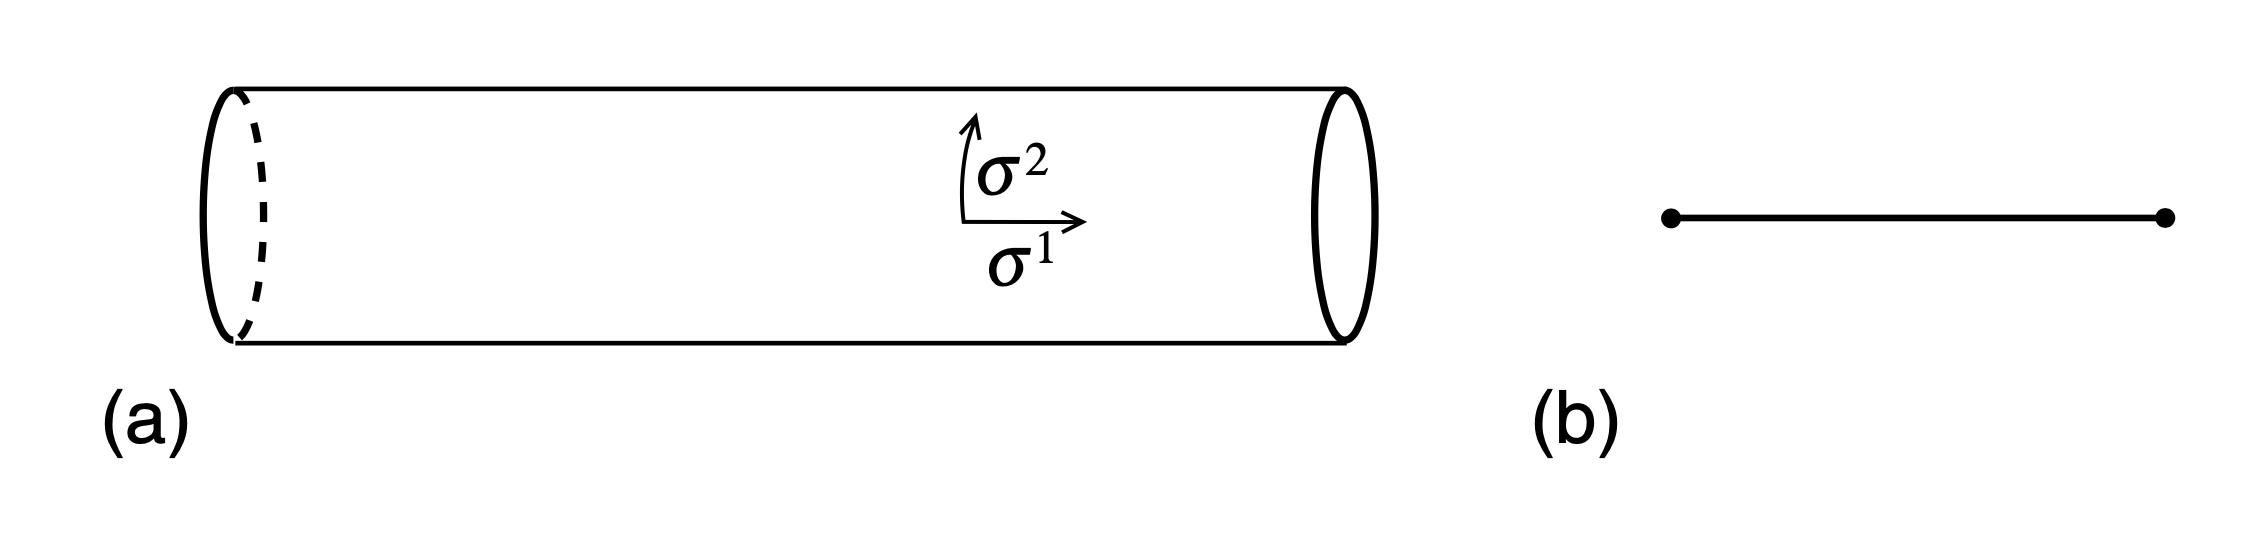
\includegraphics[width=0.6\textwidth]{figure/fig101.png}
		\caption{(a) Cylinder in the small $t$ limit. (b) Field theory analogy diagram.}
	\end{figure}
	
	First examine the cylinder, combined with the results for bosonic strings (\textcolor{red}{7.4.1}) in ten dimensions, plus the fermionic trace (\ref{10.7.9}); the trace here comes from one side of a Type II string, and we write it as a sum of two terms
	\begin{equation}
		Z_{C_{2}}=Z_{C_{2},0}+Z_{C_{2},1} \:, \label{10.8.1}
	\end{equation}
	where
	\begin{subequations}
		\begin{align}
			Z_{C_{2},0}&=\mi V_{10} n^{2}\int^{\infty}_{0}\frac{\dif t}{8t}(8\pi^{2}\alpha^{\prime}t)^{-5}\eta(\mi t)^{-8}
			\Bigl[Z^{0}{}_{0}(\mi t)^{4}-Z^{1}{}_{0}(\mi t)^{4}\Bigr] \:, \label{10.8.2a} \\
			Z_{C_{2},1}&=\mi V_{10} n^{2}\int^{\infty}_{0}\frac{\dif t}{8t}(8\pi^{2}\alpha^{\prime}t)^{-5}\eta(\mi t)^{-8}
			\Bigl[-Z^{0}{}_{1}(\mi t)^{4}-Z^{1}{}_{1}(\mi t)^{4}\Bigr] \:, \label{10.8.2b}
		\end{align} \label{10.8.2}
	\end{subequations}
	(Note that Type I superstrings can only be unoriented; they come from Type IIB string theory, so there is a negative sign in front of $Z^{1}{}_{1}$.) We separated these four terms according to whether $\exp(\pi\mi F)$ appeared in the trace. $\exp(\pi\mi F)$ is not in $Z_{C_{2},0}$, so $\psi^{\mu}$ is antiperiodic in the $\sigma_{2}$ direction. This term is in $Z_{C_{2},1}$, so $\psi^{\mu}$ is periodic in the $\sigma_{2}$ direction. We can also think of the cylinder as closed strings being produced from vacuum and then annihilated back to vacuum. The periodicity of $\psi^{\mu}$ indicates that $Z_{C_{2},0}$ comes from NS-NS strings and $Z_{C_{2},1}$ comes from R-R closed strings.
	
	Due to supersymmetry, the total fermionic string partition function is zero, which makes $Z_{C_{2},1}=-Z_{C_{2},0}$; we now concentrate on $Z_{C_{2},0}$. Using modular transformation
	\begin{equation}
		\eta_{\mi t} =t^{-1/2} \eta(\mi/t) \:, \qquad Z^{\alpha}{}_{\beta}(\mi t) = Z^{\beta}{}_{-\alpha}(\mi/t)\label{10.8.3}
	\end{equation}
	Define $s=\pi/t$, which becomes
	\begin{align}
		Z_{C_{2},0} &= \mi \frac{V_{10}n^{2}}{8\pi(8\pi^{2}\alpha^{\prime})^{5}}
		\int \dif s\:\eta(\mi s/\pi)^{-8}\Bigl[Z^{0}{}_{0}(\mi s/\pi)^{4}- Z^{0}{}_{1}(\mi s/\pi)^{4} \Bigr] \nonumber \\
		&=\mi \frac{V_{10}n^{2}}{8\pi(8\pi^{2}\alpha^{\prime})^{5}}
		\int \dif s\: [16 + O(\exp(-2s))] \:. \label{10.8.4}
	\end{align}
	\begin{tcolorbox}[breakable]
		\begin{remark}
			\textbf{Change of variables.} Apply (\ref{10.8.3}) with $\tau=\mi t\to-1/\tau=\mi/t$. By the box after (\ref{10.7.14}), $Z^0{}_0(\mi t)=Z^0{}_0(\mi/t)$ and $Z^1{}_0(\mi t)=Z^0{}_1(\mi/t)$. Then
			\begin{align*}
				\frac{\dif t}{8t}(8\pi^{2}\alpha't)^{-5}\eta(\mi t)^{-8}
				&\eqs{1}\frac{\dif t}{8t}(8\pi^{2}\alpha')^{-5}t^{-5}\,t^{4}\,\eta(\mi/t)^{-8}
				=\frac{(8\pi^{2}\alpha')^{-5}}{8}\frac{\dif t}{t^{2}}\,\eta(\mi/t)^{-8}\\
				&\eqs{2}\frac{(8\pi^{2}\alpha')^{-5}}{8\pi}\,\dif s\;\eta(\mi s/\pi)^{-8} .
			\end{align*}
			At (1), $\eta(\mi t)^{-8}=t^{4}\eta(\mi/t)^{-8}$. At (2), $s=\pi/t$, so $\dif t/t^{2}=-\dif s/\pi$, and the orientation flip was absorbed by swapping the limits. Together with the bracket $Z^0{}_0{}^4-Z^0{}_1{}^4$, this is the first line of (\ref{10.8.4}).

			\textbf{Large $s$.} Here $\tau=\mi s/\pi$ and $q=\me^{2\pi\mi\tau}=\me^{-2s}$. From the $q$-expansions in the proof after (\ref{10.7.16}),
			\begin{equation*}
				\eta^{-8}\bigl(Z^0{}_0{}^{4}-Z^0{}_1{}^{4}\bigr)=\frac{\vartheta_{00}^{4}-\vartheta_{01}^{4}}{\eta^{12}}=\frac{16q^{1/2}+128q^{3/2}+\cdots}{q^{1/2}\prod(1-q^m)^{8}}=16+O(q)=16+O(\me^{-2s}) .
			\end{equation*}
			The constant $16$ is the massless closed-string state exchanged over the long tube. It gives the divergence $\int^\infty\dif s$. The next term is $\me^{-2s}$, which is the propagation of the first massive level.
		\end{remark}
	\end{tcolorbox}
	Divergence as $s\to\infty$ is due to massless closed string tadpoles; note that this must be an NS-NS state. We view it as dilaton-graviton interaction $(-G)^{1/2}\me^{-\Phi}$.
	
	However, there is a contradiction here: $d=10, N=1$ supersymmetric algebra does not allow such a term. Even more strangely, $Z_{C_{2},1}$ has a divergence of equal size and opposite sign, which can only come from R-R state tadpoles, but the only massless R-R state is a 2nd-order tensor, which cannot have Lorentz-invariant tadpoles.
	
	One can guess the solution is like this. Type IIB strings have $n$-th rank potentials for all even $n$, and $n$ and $8-n$ are equal under Poincaré duality. $\Omega$ projection removed $n=0$ and equivalent $n=8$, as well as $n=4$: all multiples of 4. $n=2$, equivalent $n=6$ and $n=10$ are left. A 10-form potential $C_{10}$ is allowed in 10 dimensions, but its 11-form field strength $\dif C_{10}$ is identically zero. The integration of this potential over spacetime
	\begin{equation}
		\mu_{10}\int C_{10} \label{10.8.5}
	\end{equation}
	is invariant under $\delta C_{10}=\dif \chi_{9}$, so it can appear in action. Because there is no kinetic energy term, the propagator for this field is $1/0$, and the divergence of the tadpole is
	\begin{equation}
		\frac{\mu^{2}_{10}}{0} \:. \label{10.8.6}
	\end{equation}
	This is exactly the origin of divergence in $Z_{C_{2},1}$. The equation of motion given by the variation of $C_{10}$ is $\mu_{10}=0$, so unlike previously encountered divergences, this one cannot be removed by background field corrections. It represents a real incompatibility.
	
	\subsection*{The Klein bottle}
	
	There is another way to cancel tadpole divergences. Cylinders, Mobius strips and Klein bottles all have divergences from massless closed string states, with the total divergence being proportional to the square of the sum of the disk tadpole and the $RP_{2}$ tadpole. The relative size of the two tadpoles depends on the Chan-Paton factors, canceling each other for specific gauge groups.
	
	To sum these contributions, we must readjust these surfaces so that the perimeter in the $\sigma^{2}$ direction and the length in the $\sigma^{1}$ direction are consistent; we take them to be $2\pi$ and $s$, respectively. For the cylinder, the original length of $\sigma^{1}$ was $\pi$ (due to the cylinder corresponding to open strings), and the length in the $\sigma^{2}$ direction was $2\pi t$, so we get $s=\pi/t$; for the Klein bottle $s=\pi/2t$; and for the Mobius strip $s=\pi/4t$. 
	
	Each amplitude is a sum over traces, which come from different boundary conditions and projections. We need to determine which terms contribute to NS-NS exchanges and which contribute to R-R exchanges by examining boundary conditions of fermions on worldsheet path integrals. On the Klein bottle, the GSO projection operator is
	\begin{equation}
		\frac{1+\exp(\pi\mi F)}{2} \:,\qquad \frac{1+\exp(\pi\mi\tilde{F})}{2} \:. \label{10.8.7}
	\end{equation}
	Adding $R=\Omega \exp(\pi\mi\beta F +\pi\mi\tilde{\beta}\tilde{F})$ to the trace, path integral boundary conditions are
	\begin{subequations}
		\begin{align}
			\psi(w+2\pi\mi t)&= -R\psi(w)R^{-1} =-\exp(\pi\mi\beta)\tilde{\psi}(\bar{w}) \:, \label{10.8.8a} \\
			\tilde{\psi}(\bar{w}+2\pi\mi t)&= -R\tilde{\psi}(\bar{w})R^{-1} =-\exp(\pi\mi\tilde{\beta})\psi(w)\:,\label{10.8.8b}
		\end{align} \label{10.8.8}
	\end{subequations}
	negative signs appear because of the fermion field. This gives
	\begin{equation}
		\psi(w+4\pi\mi t) = \exp[\pi\mi(\beta+\tilde{\beta})]\,\psi(w) \:. \label{10.8.9}
	\end{equation}
	NS-NS exchange comes from sectors antisymmetric under $\sigma^{2}\to\sigma^{2}+4\pi t$, and thus from traces factoring in weight $\Omega\exp(\pi\mi F)$ or $\Omega\exp(\pi\mi\tilde{F})$; furthermore, these two traces are equal. Both NS-NS and R-R states contribute to this trace, and their respective contributions are
	\begin{subequations}
		\begin{align}
			\text{NS-NS }: \qquad &q^{-1/3}\prod_{m=1}^{\infty} (1+q^{2m-1})^{8} = Z^{0}{}_{0}(2\mi t)^{4} \:, \label{10.8.10a} \\
			\text{R-R }: \qquad &-16 q^{2/3} \prod_{m=1}^{\infty} (1+q^{2m})^{8} =- Z^{1}{}_{0}(2\mi t)^{4} \:,
			\label{10.8.10b}
		\end{align} \label{10.8.10}
	\end{subequations}
	where $q=\exp(-2\pi t)$.
	
	Thus, the entire Klein bottle contribution to NS-NS exchange is
	\begin{align}
		Z_{K_{2},0} &= \mi V_{10} \int_{0}^{\infty}\frac{\dif t}{8t}\: (4\pi^{2}\alpha^{\prime}t)^{-5} \eta(2\mi t)^{-8}
		\Bigl[ Z^{0}{}_{0}(2\mi t)^{4}-Z^{1}{}_{0}(2\mi t)^{4}\Bigr] \nonumber \\
		&= \mi \frac{2^{10}V_{10}}{8\pi (8\pi^{2}\alpha^{\prime})^{5}}\int^{\infty}_{0}\dif s \: 
		\eta(\mi s/\pi)^{-8} \Bigl[ Z^{0}{}_{0}(\mi s/\pi)^{4}-Z^{1}{}_{0}(\mi s/\pi)^{4} \Bigr] \nonumber \\
		&= \mi \frac{2^{10}V_{10}}{8\pi (8\pi^{2}\alpha^{\prime})^{5}}\int^{\infty}_{0}\dif s \: 
		[16 + O(\exp(-2s))] \:, \label{10.8.11}
	\end{align}
	and $Z_{K_{2},1}=-Z_{K_{2},0}$. The bosonic part is the same as before.
	\begin{tcolorbox}[breakable]
		\begin{remark}
			\textbf{Why $\tau=2\mi t$ in (\ref{10.8.10}).} $\Omega$ exchanges left and right movers, $\Omega\lvert i\rangle_L\lvert j\rangle_R=\pm\lvert j\rangle_L\lvert i\rangle_R$. So in $\operatorname{Tr}\bigl(\Omega\,q^{L_0+\tilde L_0}\bigr)$ only the diagonal states $i=j$ contribute, and each carries $q^{2L_0}=(q^{2})^{L_0}$. The Klein-bottle trace is therefore a single chiral trace at nome $q^{2}=\me^{-4\pi t}$, i.e.\ at $\tau=2\mi t$.

			\textbf{(\ref{10.8.10}).} With $Q\equiv q^{2}$ the nome of $\tau=2\mi t$, and the products of (\ref{10.7.7b}),
			\begin{align*}
				Z^0{}_0(2\mi t)^{4}&=Q^{-1/6}\prod_m(1+Q^{m-1/2})^{8}=q^{-1/3}\prod_m(1+q^{2m-1})^{8},\\
				Z^1{}_0(2\mi t)^{4}&=\bigl(2Q^{1/12}\bigr)^{4}\prod_m(1+Q^{m})^{8}=16q^{2/3}\prod_m(1+q^{2m})^{8} .
			\end{align*}
			The R-R sign is the spacetime statistics of the R sector, as in (\ref{10.7.9}).

			\textbf{(\ref{10.8.11}).} Now $\tau=2\mi t\to-1/\tau=\mi/2t$:
			\begin{align*}
				\frac{\dif t}{8t}(4\pi^{2}\alpha't)^{-5}\eta(2\mi t)^{-8}
				&\eqs{1}\frac{\dif t}{8t}\,2^{5}(8\pi^{2}\alpha')^{-5}t^{-5}\,(2t)^{4}\,\eta(\mi/2t)^{-8}
				=\frac{2^{9}(8\pi^{2}\alpha')^{-5}}{8}\frac{\dif t}{t^{2}}\eta(\mi/2t)^{-8}\\
				&\eqs{2}\frac{2^{10}(8\pi^{2}\alpha')^{-5}}{8\pi}\,\dif s\;\eta(\mi s/\pi)^{-8} .
			\end{align*}
			At (1), $(4\pi^{2}\alpha')^{-5}=2^{5}(8\pi^{2}\alpha')^{-5}$ and $\eta(2\mi t)^{-8}=(2t)^{4}\eta(\mi/2t)^{-8}$. At (2), $s=\pi/2t$, so $\dif t/t^{2}=2\,\dif s/\pi$ up to orientation, and $\mi/2t=\mi s/\pi$. The bracket becomes $Z^0{}_0{}^4-Z^0{}_1{}^4$ at $\mi s/\pi$, exactly as for the cylinder, which gives the same $16+O(\me^{-2s})$. So the Klein bottle is the cylinder result with $n^{2}\to2^{10}=32^{2}$.
		\end{remark}
	\end{tcolorbox}
	
	
	\subsection*{The M\"{o}bius strip}
	
	In open strings, the effect of $\Omega$ is
	\begin{equation}
		\Omega\psi^{\mu}(w)\Omega^{-1} =\tilde{\psi}(\pi-\bar{w})=\psi^{\mu}(w-\pi) \:,\label{10.8.12}
	\end{equation}
	doubling trick (\ref{10.2.15}) was used here. In form of oscillator modes, this is
	\begin{equation}
		\Omega \psi^{\mu}_{r} \Omega^{-1} =\exp(-\pi\mi r) \,\psi_{r}^{\mu} \:. \label{10.8.13}
	\end{equation}
	This phase is imaginary and its square is equal to $-1$ in the NS sector. Therefore,
	\begin{equation}
		\Omega^{2} =\exp(\pi\mi F) \:. \label{10.8.14}
	\end{equation}
	\begin{tcolorbox}[breakable]
		\begin{remark}
			\textbf{(\ref{10.8.13}).} With the doubled field of (\ref{10.2.15}) and the expansion (\ref{10.2.5}),
			\begin{equation*}
				\Omega\psi^\mu(w)\Omega^{-1}=\psi^\mu(w-\pi)=\mi^{-1/2}\sum_r\psi^\mu_r\me^{\mi r(w-\pi)}
				\quad\Longrightarrow\quad \Omega\psi^\mu_r\Omega^{-1}=\me^{-\pi\mi r}\psi^\mu_r .
			\end{equation*}
			\textbf{(\ref{10.8.14}).} Applying this twice gives $\Omega^{2}\psi_r\Omega^{-2}=\me^{-2\pi\mi r}\psi_r$. This is $-\psi_r$ for $r\in\mathds Z+\tfrac12$ and $+\psi_r$ for $r\in\mathds Z$. On NS states $\Omega^{2}$ therefore gives $-1$ per $\psi$ excitation, which is the action of $\exp(\pi\mi F)$ on them. The phase of $\Omega$ on the ground state is a convention, fixed so that (\ref{10.8.14}) holds on all states. $\Omega$ is then of order 4 on the full space, which is why the projector (\ref{10.8.15}) averages over $\Omega^{0,1,2,3}$. On GSO-projected states it reduces to $\tfrac12(1+\Omega)$.

			\textbf{(\ref{10.8.16}).} In the trace with $R=\Omega\exp(\pi\mi\beta F)$, going once around the $\sigma^{2}$ circle of circumference $2\pi t$ gives $\psi(w+2\pi\mi t)=-\exp(\pi\mi\beta)\,\psi(w-\pi)$. The $-$ is the fermionic trace, and the argument is from (\ref{10.8.12}). Going around twice,
			\begin{equation*}
				\psi(w+4\pi\mi t)=-\me^{\pi\mi\beta}\psi(w+2\pi\mi t-\pi)=\bigl(-\me^{\pi\mi\beta}\bigr)^{2}\psi(w-2\pi)=\psi(w-2\pi),
			\end{equation*}
			for $\beta\in\{0,1\}$. By (\ref{10.2.3a}), $\psi(w-2\pi)=\me^{-2\pi\mi\nu}\psi(w)$. So along the doubled $\sigma^{2}$ circle, which is the closed-string time direction of the M\"obius strip, R-sector fields ($\nu=0$) are periodic and NS-sector fields are antiperiodic. In the closed-string channel the R sector of the open-string trace is R-R exchange, and the NS sector is NS-NS exchange.
		\end{remark}
	\end{tcolorbox}
	According to GSO projection, $\exp(\pi\mi F)=1$; physically, its square is the same as the identity operator, but the combined projection of $\Omega$ and GSO requires
	\begin{equation}
		\frac{1+\Omega +\Omega^{2}+\Omega^{3}}{4} \:. \label{10.8.15}
	\end{equation}
	Now there's $R=\Omega \exp(\pi\mi\beta F)$ in the trace, and the periodicity of the field is
	\begin{equation}
		\psi^{\mu}(w+4\pi\mi t) = -\exp(\pi\mi\beta)\psi^{\mu}(w+2\pi\mi t-\pi) =\psi^{\mu}(w-2\pi) \:. \label{10.8.16}
	\end{equation}
	It follows that in the R sector of trace, the field is periodic in the $\sigma^{2}$ direction, corresponding to R-R exchange, while the NS sector of trace gives NS-NS exchange.
	
	R-R exchange is simpler, and the sum of traces containing $\Omega$ and $\Omega\exp(\pi\mi F)$ is
	\begin{align}
		-16q^{1/3}&\prod_{m=1}^{\infty} [1+(-1)^{m}q^{m}]^{8} 
		-(1-1)^{4}q^{1/3}\prod_{m=1}^{\infty} [1-(-1)^{m}q^{m}]^{8} \nonumber \\
		&= Z^{0}{}_{1}(2\mi t)^{4} Z^{1}{}_{0}(2\mi t)^{4} \:. \label{10.8.17}
	\end{align}
	The overall Mobius amplitude is
	\begin{align}
		Z_{M_{2},1}&=\pm\mi n V_{10} \int_{0}^{\infty} \frac{\dif t}{8t}(8\pi^{2}\alpha^{\prime}t)^{-5}
		\frac{Z^{0}{}_{1}(2\mi t)^{4}Z^{1}{}_{0}(2\mi t)^{4}}{\eta(2\mi t)^{8}Z^{0}{}_{0}(2\mi t)^{4}}\nonumber \\
		&=\pm 2\mi n \frac{2^{5}V_{10}}{8\pi(8\pi^{2}\alpha^{\prime})^{5}}\int_{0}^{\infty}\dif s \:
		\frac{Z^{0}{}_{1}(2\mi s/\pi)^{4}Z^{1}{}_{0}(2\mi s/\pi)^{4}}{\eta(2\mi s/\pi)^{8}Z^{0}{}_{0}(2\mi s/\pi)^{4}}\nonumber \\
		&=\pm 2\mi n \frac{2^{5}V_{10}}{8\pi(8\pi^{2}\alpha^{\prime})^{5}}\int_{0}^{\infty}\dif s \:
		[16+O(\exp(-2s))] \:, \label{10.8.18}
	\end{align}
	where the positive sign corresponds to $SO(n)$.
	
	The total divergence of R-R exchange is
	\begin{equation}
		Z_{1} = -\mi(n\mp 32)^{2} \frac{V_{10}}{8\pi (8\pi^{2}\alpha^{\prime})^{5}}
		\int^{\infty}_{0}\dif s \:[16+O(\exp(-2s))] \:. \label{10.8.19}
	\end{equation}
	\begin{tcolorbox}[breakable]
		\begin{remark}
			\textbf{Conventions.} Open-string traces are at $q=\me^{-2\pi t}$, with the eight transverse directions. $Q\equiv q^{2}$ is the nome at $\tau=2\mi t$. By (\ref{10.8.13}), $\Omega$ multiplies an integer mode $n$ by $(-1)^n$, and the same holds for the $X$ oscillators.

			\textbf{The R-R trace (\ref{10.8.17}).} The R ground states carry $2^{8/2}=16$ states and zero-point energy $8\cdot\tfrac1{24}=\tfrac13$, and the spacetime statistics give a $-$ sign. In the $\Omega\exp(\pi\mi F)$ trace the zero modes give $\operatorname{Tr}_{16}\Gamma=0$, which is the $(1-1)^{4}$. The surviving piece, times the bosonic M\"obius trace $q^{-1/3}\prod_m(1-(-1)^mq^m)^{-8}$, is
			\begin{align*}
				-16\prod_m\Bigl[\frac{1+(-1)^mq^m}{1-(-1)^mq^m}\Bigr]^{8}
				&\eqs{1}-16\prod_m\Bigl[\frac{(1+Q^{m})(1-Q^{m-1/2})}{(1-Q^{m})(1+Q^{m-1/2})}\Bigr]^{8}\\
				&\eqs{2}-\frac{Z^0{}_1(2\mi t)^{4}\,Z^1{}_0(2\mi t)^{4}}{\eta(2\mi t)^{8}\,Z^0{}_0(2\mi t)^{4}} .
			\end{align*}
			At (1), the even $m=2k$ and odd $m=2k-1$ factors were separated, with $q^{2k}=Q^{k}$ and $q^{2k-1}=Q^{k-1/2}$. At (2), the products of (\ref{10.7.7b}) at nome $Q$ were used: $Z^0{}_1{}^4Z^1{}_0{}^4/Z^0{}_0{}^4=16\,Q^{1/3}\prod(1+Q^m)^{8}(1-Q^{m-1/2})^{8}(1+Q^{m-1/2})^{-8}$ and $\eta^{8}=Q^{1/3}\prod(1-Q^m)^{8}$.

			\textbf{Printed-equation note.} (\ref{10.8.17}) as printed equates the fermionic trace alone to $Z^0{}_1{}^4Z^1{}_0{}^4$. The identity holds only after the bosonic M\"obius trace is included, and then with the ratio above, which is what enters (\ref{10.8.18}). The overall sign is absorbed into the $\pm$ of (\ref{10.8.18}), which is fixed by the $SO/Sp$ action of $\Omega$ on the Chan--Paton factors.

			\textbf{(\ref{10.8.18}).} With $\tau=2\mi t\to\mi/2t$, the ratio of $Z$'s is invariant because $Z^0{}_1\leftrightarrow Z^1{}_0$. Then
			\begin{align*}
				\frac{\dif t}{8t}(8\pi^{2}\alpha't)^{-5}\eta(2\mi t)^{-8}
				&\eqs{1}\frac{2^{4}(8\pi^{2}\alpha')^{-5}}{8}\frac{\dif t}{t^{2}}\eta(\mi/2t)^{-8}
				\eqs{2}\frac{2\cdot2^{5}(8\pi^{2}\alpha')^{-5}}{8\pi}\dif s\;\eta(2\mi s/\pi)^{-8} .
			\end{align*}
			At (1), $\eta(2\mi t)^{-8}=(2t)^{4}\eta(\mi/2t)^{-8}$. At (2), $s=\pi/4t$, so $\dif t/t^{2}=4\,\dif s/\pi$ and $\mi/2t=2\mi s/\pi$. At large $s$ the nome is $\me^{-4s}$. $\eta^{-8}Z^1{}_0{}^4=16(1+\cdots)$ and $Z^0{}_1{}^4/Z^0{}_0{}^4=1+O(\me^{-2s})$, so the bracket is $16+O(\me^{-2s})$.

			\textbf{(\ref{10.8.19}).} Using $Z_{C_2,1}=-Z_{C_2,0}$ and $Z_{K_2,1}=-Z_{K_2,0}$, with the common factor $\frac{\mi V_{10}}{8\pi(8\pi^{2}\alpha')^{5}}\int\dif s\,[16+\cdots]$ written as $\mi\mathcal N$:
			\begin{equation*}
				Z_1=-\mi\mathcal N\bigl(n^{2}+2^{10}\bigr)\pm\mi\mathcal N\,2\cdot2^{5}n=-\mi\mathcal N\bigl(n^{2}\mp64n+1024\bigr)=-\mi\mathcal N\,(n\mp32)^{2} .
			\end{equation*}
			The upper sign is $SO(n)$. The R-R tadpole cancels only for $SO(32)$: the three surfaces combine into a perfect square because the divergence is (disk tadpole $+$ $RP_2$ tadpole)$^{2}$.
		\end{remark}
	\end{tcolorbox}
	The R-R tadpole is zero for the gauge group $SO(32)$. For each worldsheet topology, NS-NS divergence is the negative of the R-R divergence, so dilaton-graviton tadpoles are also zero for $SO(32)$.